\clearpage
\section{Higgs-Tagging}
\label{sec:higgstagging}

For this analysis, we utilize a new Higgs tagging procedure that combines the information contained in energy correlation functions (ECFs) for identifying $N$-pronged substructure, with a multivariate b-tagger that classifies fat jets as originating from two b quarks. %This is the first time ECFs are used for Higgs-tagging in CMS.

\subsection{Energy correlation functions}
A detailed theoretical description of energy correlation functions,
from which most of the studies documented here are derived, is
presented in Ref.~\cite{ecf}.

%The most recent theoretical description of energy correlation functions comes in \cite{ecf}, and most of the studies documented here are based on that paper. 

For a jet $J$ with constituents $i$, we define:

\begin{equation}
  z_i = {p_T^i}\Big/{p_T^J}
\end{equation}
\begin{equation}
  e(o,N,\beta) \equiv ~_o e_N^\beta = \sum _{i_1<i_2<\cdots<i_N \in J}  \left[\prod_{1\leq k \leq j} z_{i_k}\right] \times \min\left\{\prod_{k,l\in \text{pairs}\{i_1,\dots,i_N\}}^o \Delta R_{kl}^\beta\right\} 
\end{equation}
%For a concrete example, one can look at the ECF corresponding to $o=2, N=3, \beta=1$. This is a 3-point correlation function,  but limited to taking the two smallest angles ($o=2$):
For instance, the ECF corresponding to $o=2, N=3, \beta=1$ is a
3-point correlation function, but limited to taking the two smallest
angles ($o=2$):
\begin{equation}
  _2e_3^1 =  \sum _{a<b<c \in J}  z_az_bz_c \times \min\{\Delta R_{ab}\Delta R_{ac},\Delta R_{ab}\Delta R_{bc},\Delta R_{bc}\Delta R_{ac}\}
\end{equation}

In general, we expect that an $N$-pronged jet should have $e_N \gg
e_M$ for $M>N$. Therefore, taking ratios of $(N=3)/(N=2)$ can provide a well-motivated Higgs-tagger. Ref.~\cite{ecf} proposes the specific ratio $N_2$ for this purpose:

\begin{equation}
  N_2(\beta) = \frac{e(2,3,\beta)}{e(1,2,\beta)^2}
\end{equation}

When computing ECFs for fat-jets, two modifications are made to the above formulae:
\begin{itemize}
  \item Instead of using all constituents, only those that survive soft-drop grooming are used.
  \item Only the hardest 100 constituents are considered so as to make
  the necessary computation tractable.
\end{itemize}


Figure~\ref{fig:n2tau21} (left) shows the distribution
$N_2(\beta=1.0)$ for Higgs, top-, and QCD-jets. Comparing these
distributions to soft-dropped $N$-subjettiness $\tau_{21}^{\text{SD}}$
(Fig.~\ref{fig:n2tau21}, right) shows that the discriminatory power of
$N_2$ for QCD jets is comparable to that of $\tau_{21}^{\text{SD}}$ while $N_2$ is better at separating non-QCD background
jets ({\it e.g.} top jets, see Fig.~\ref{fig:n2rocs}). Therefore, we
utilize $N_2(\beta=1)$ for tagging Higgs jets.
 
%Also shown for comparison is soft-dropped $N$-subjettiness $\tau_{21}^{\text{SD}}$. It is visible that the discrimation power of $N_2^\beta$ against QCD jets  is of the same order as the one of $\tau_{21}^{\text{SD}}$. On the other hand, $N_2$ separates better against non-QCD background jets (e.g. top jets, see Fig.~\ref{fig:n2rocs}). We therefore tag Higgs jets with the help of the $N_2(\beta=1)$ variable.

\begin{figure}
  \centering
  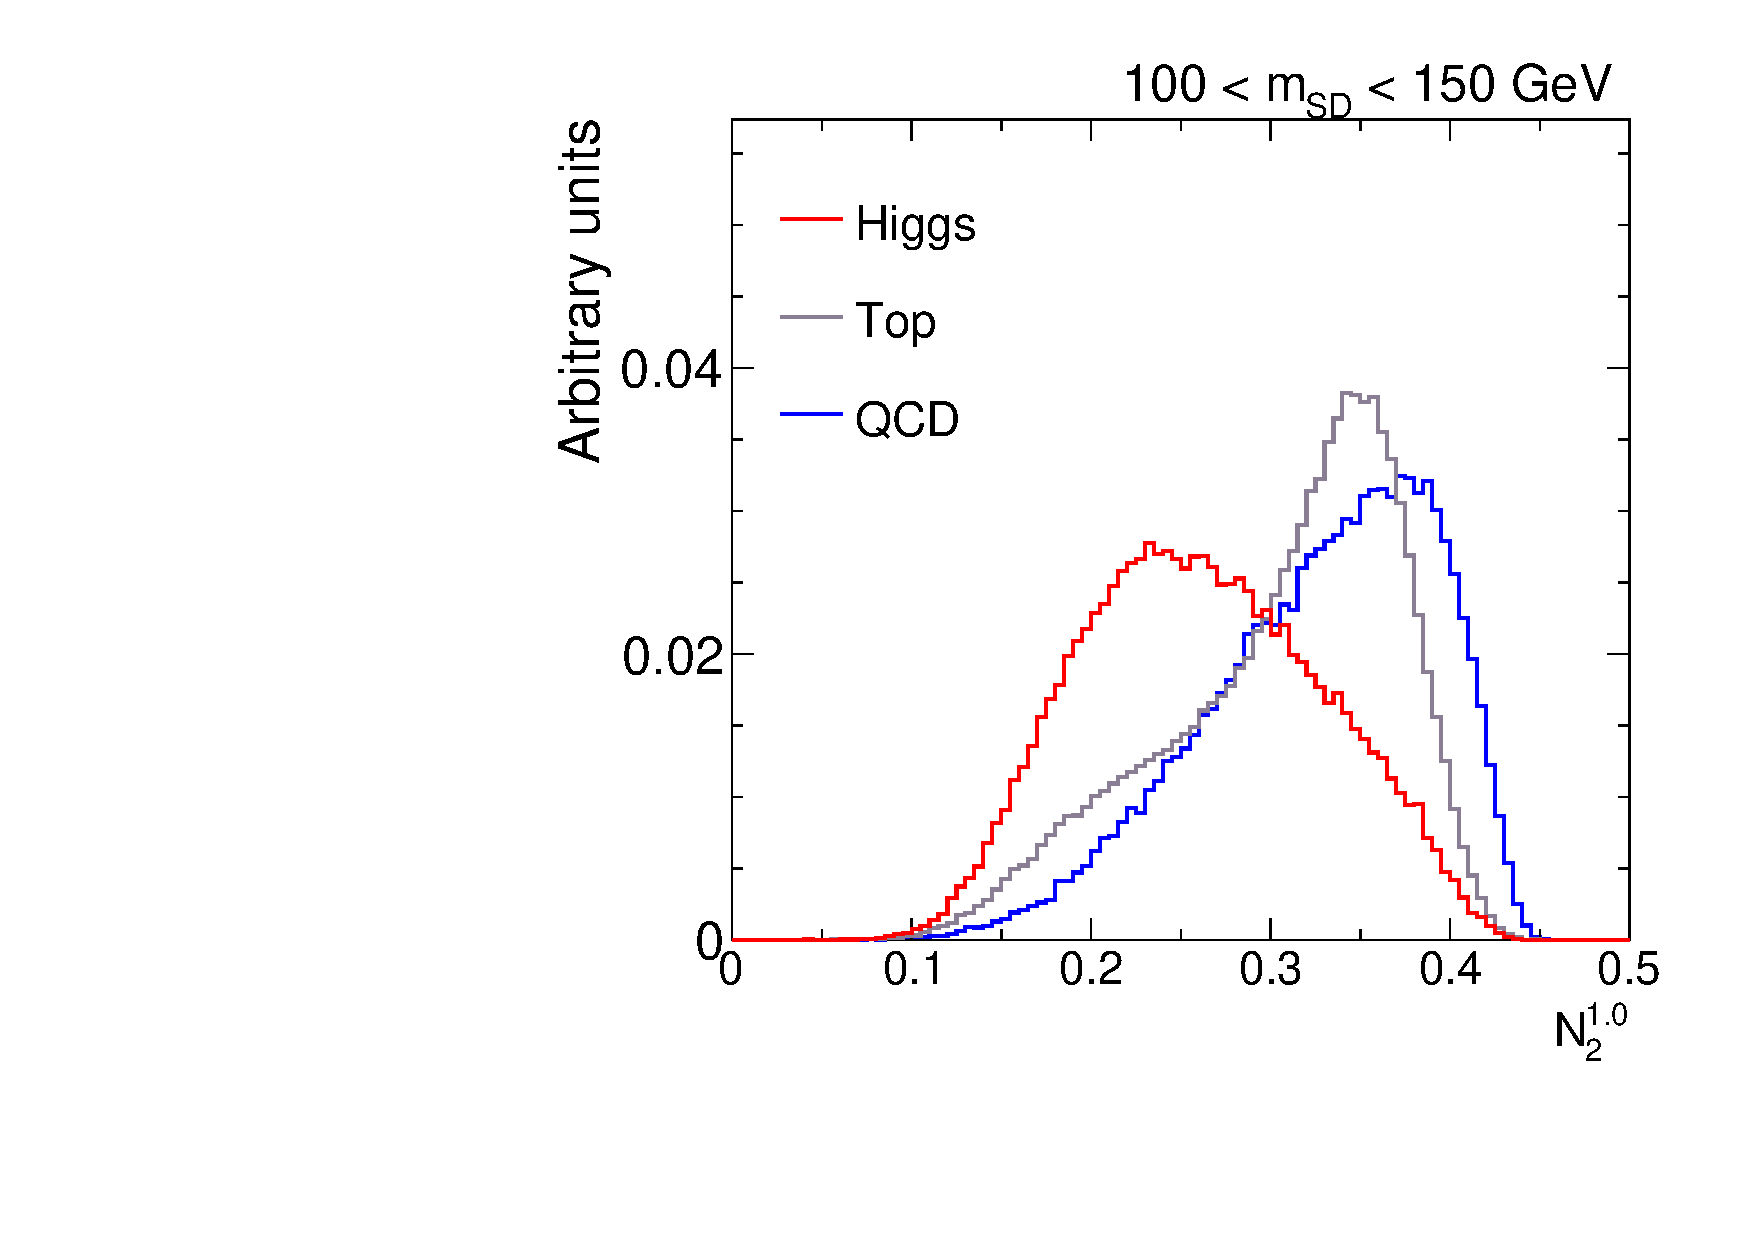
\includegraphics[width=0.475\textwidth]{figures/higgstagging/n2ddt/ddt_N2_10_ns.pdf}
  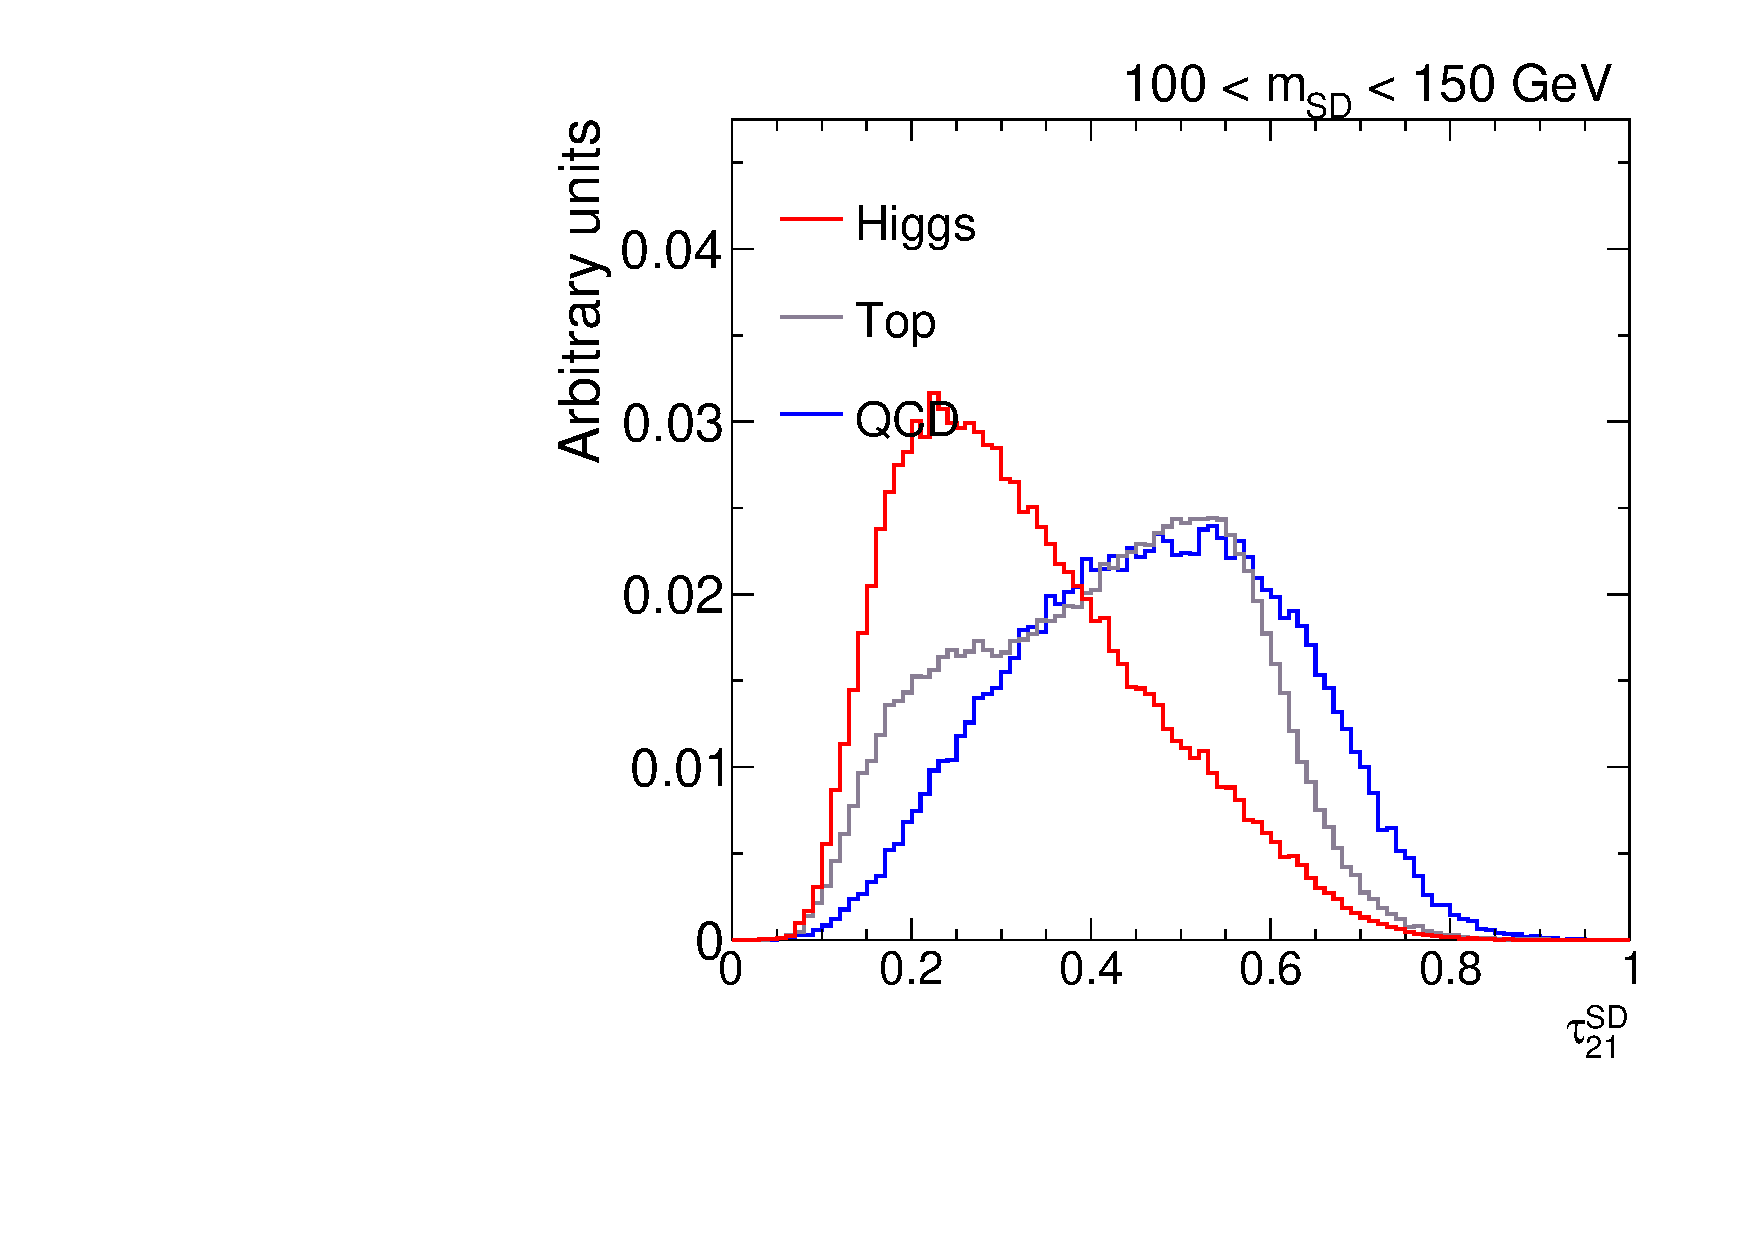
\includegraphics[width=0.475\textwidth]{figures/higgstagging/n2ddt/ddt_tau21SD_ns.pdf}
  \caption{Comparison of $N_2(\beta=1.0)$ and $\tau_{21}^\text{SD}$ for the three main types of jets in the analysis in a window around the true Higgs mass. Event weights are applied that flatten the \pt~spectrum.}
  \label{fig:n2tau21}
\end{figure}


However, as can be seen from Figure~\ref{fig:taggingkinematics}, the mass shape of QCD background fat jets varies significantly with the position of the cut on $N_2$. 

\begin{figure}
  \centering
  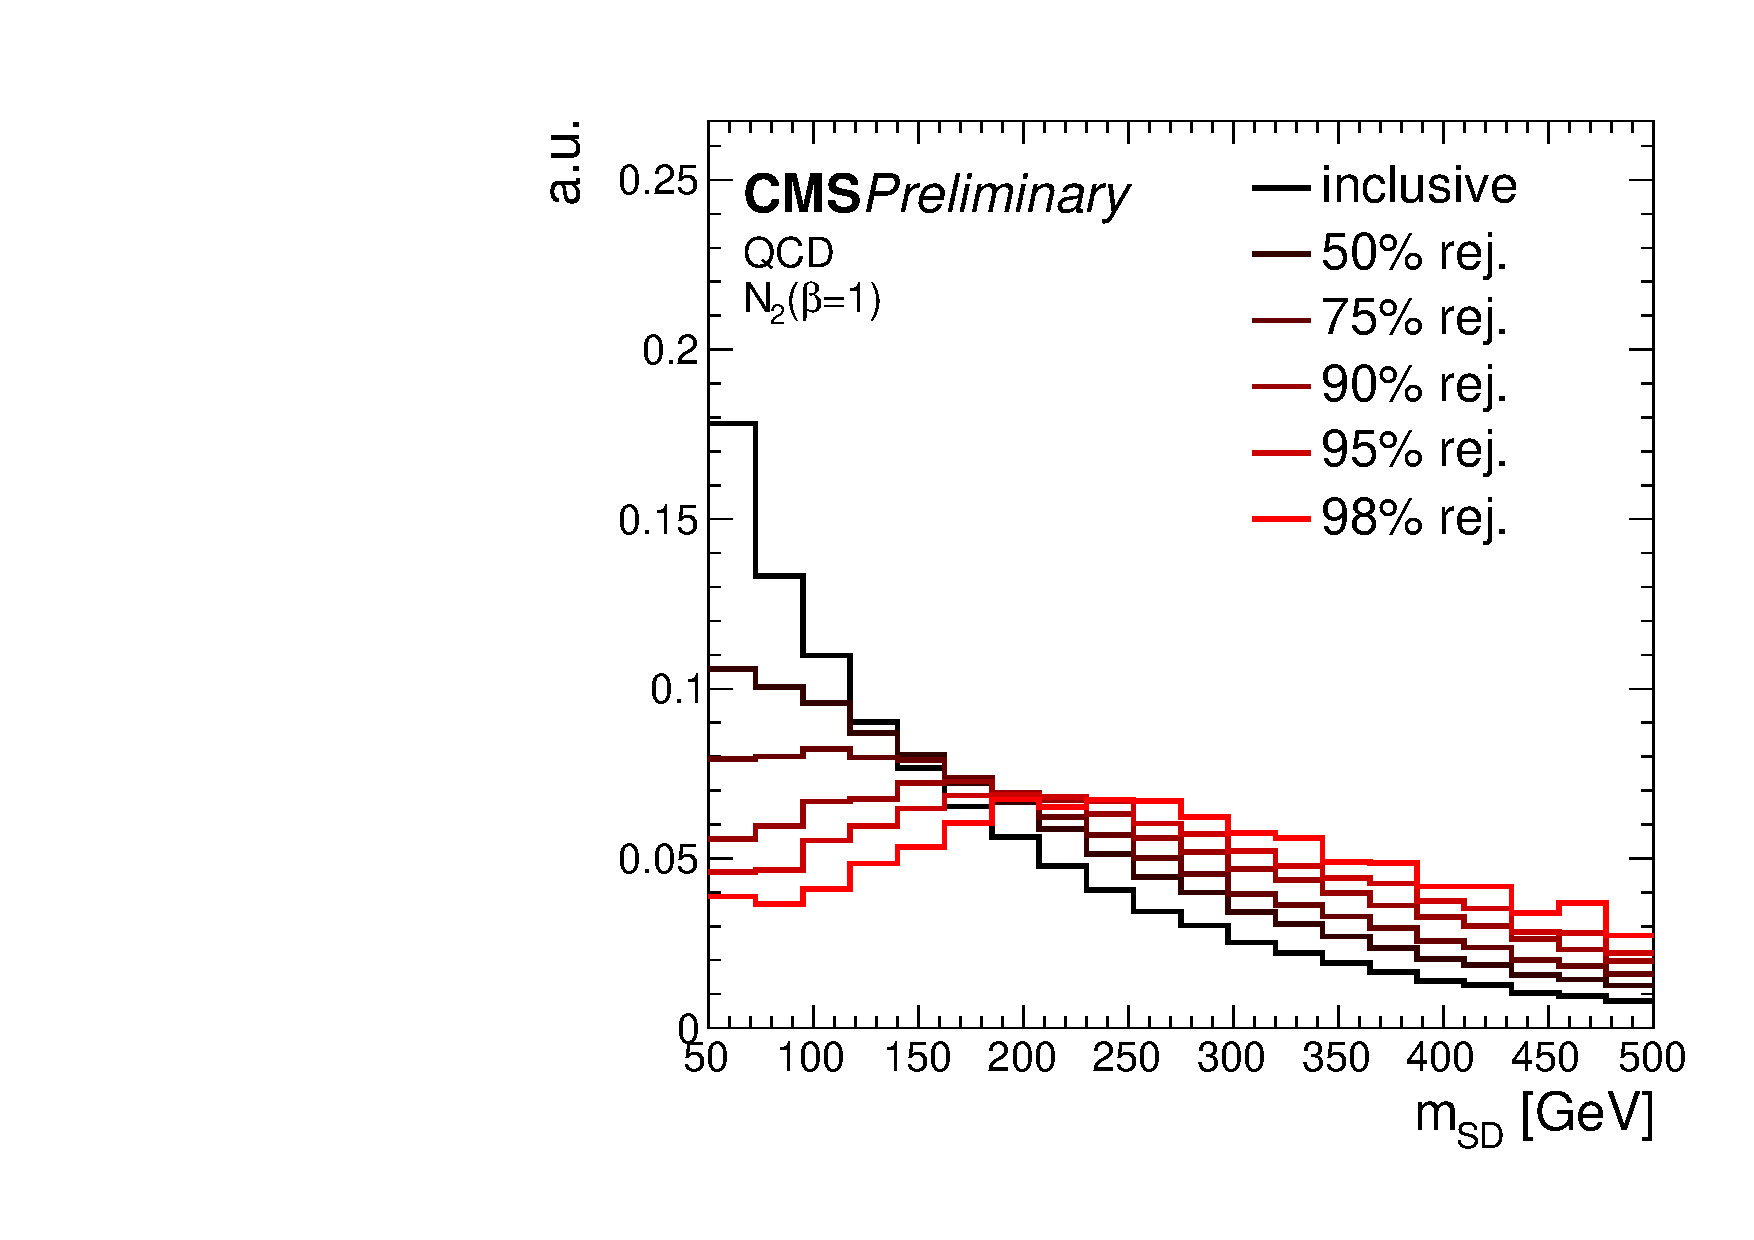
\includegraphics[width=0.475\textwidth]{figures/higgstagging/QCDN2_mSD.pdf}
  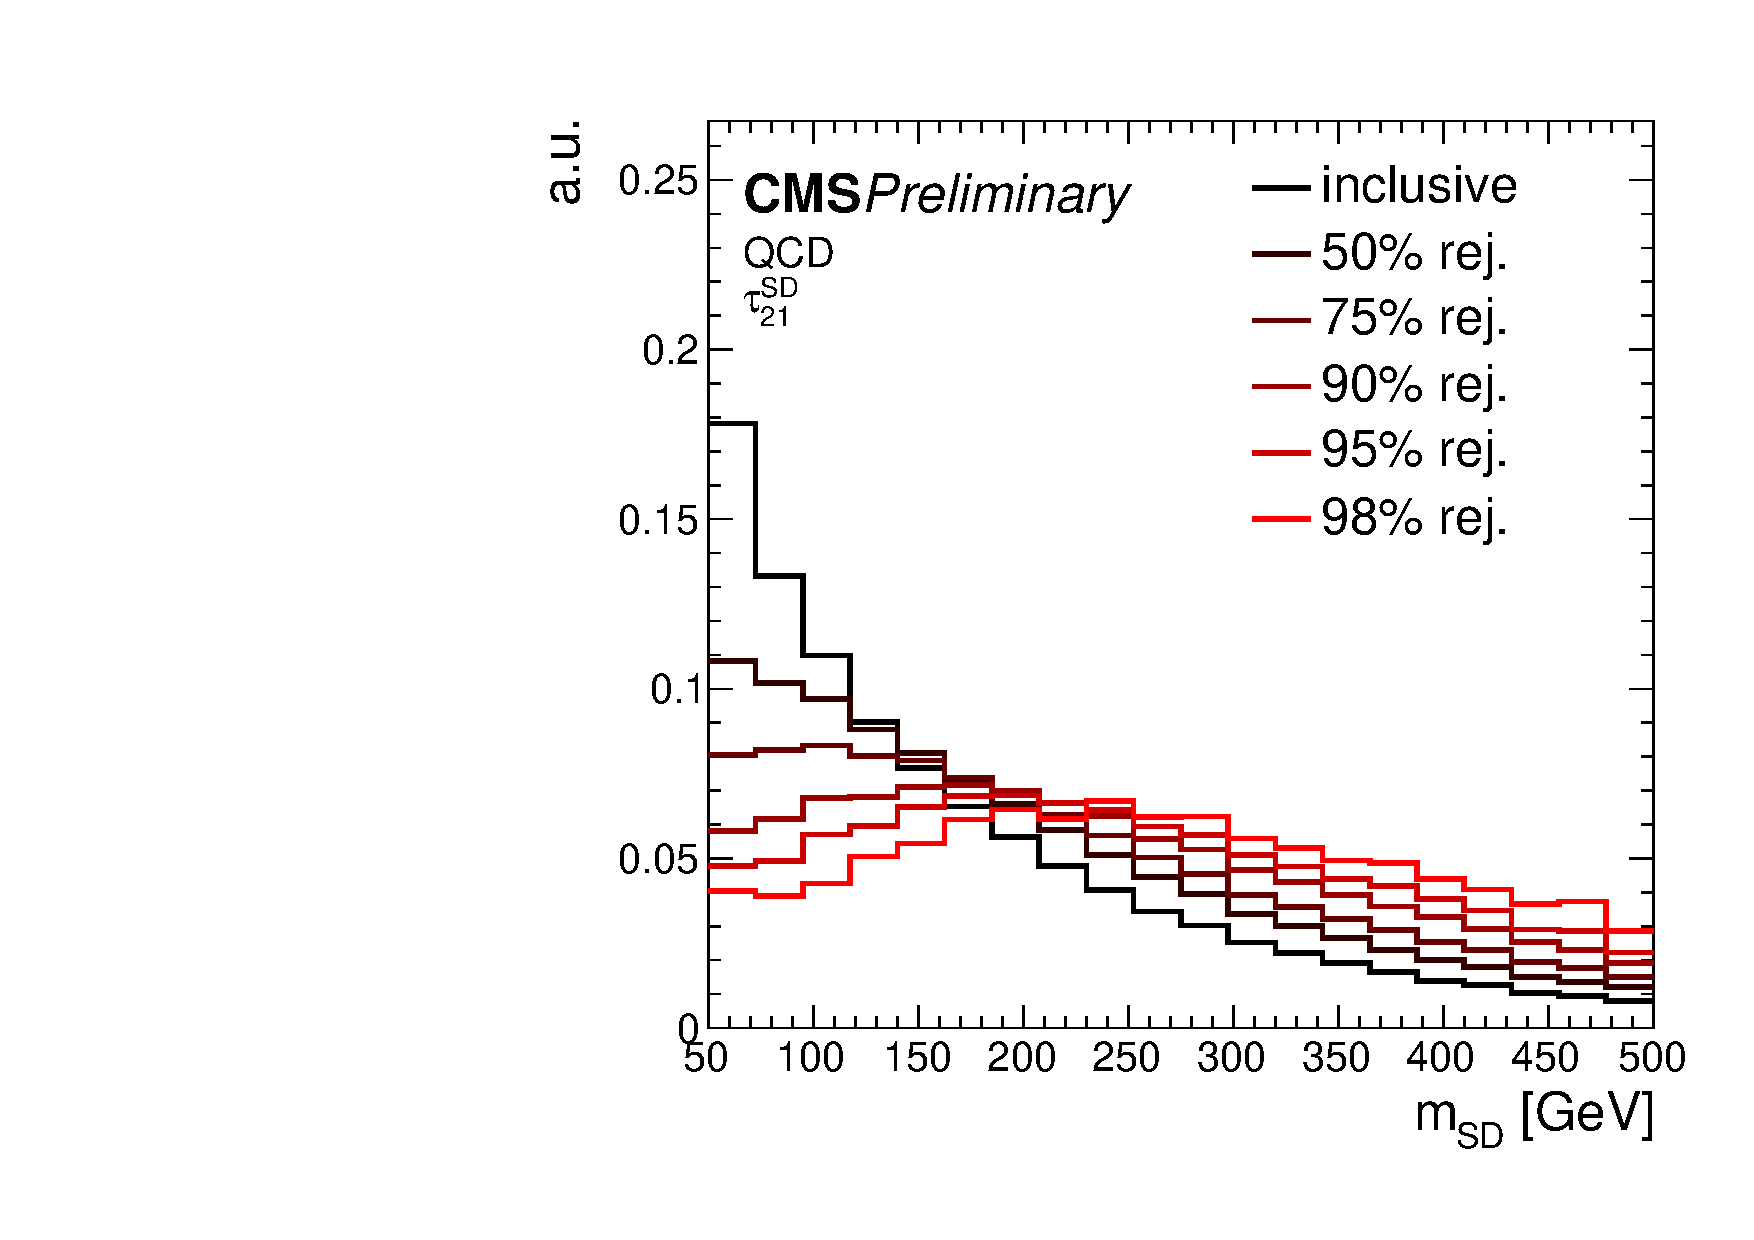
\includegraphics[width=0.475\textwidth]{figures/higgstagging/QCDtau21SD_mSD.pdf}\\
  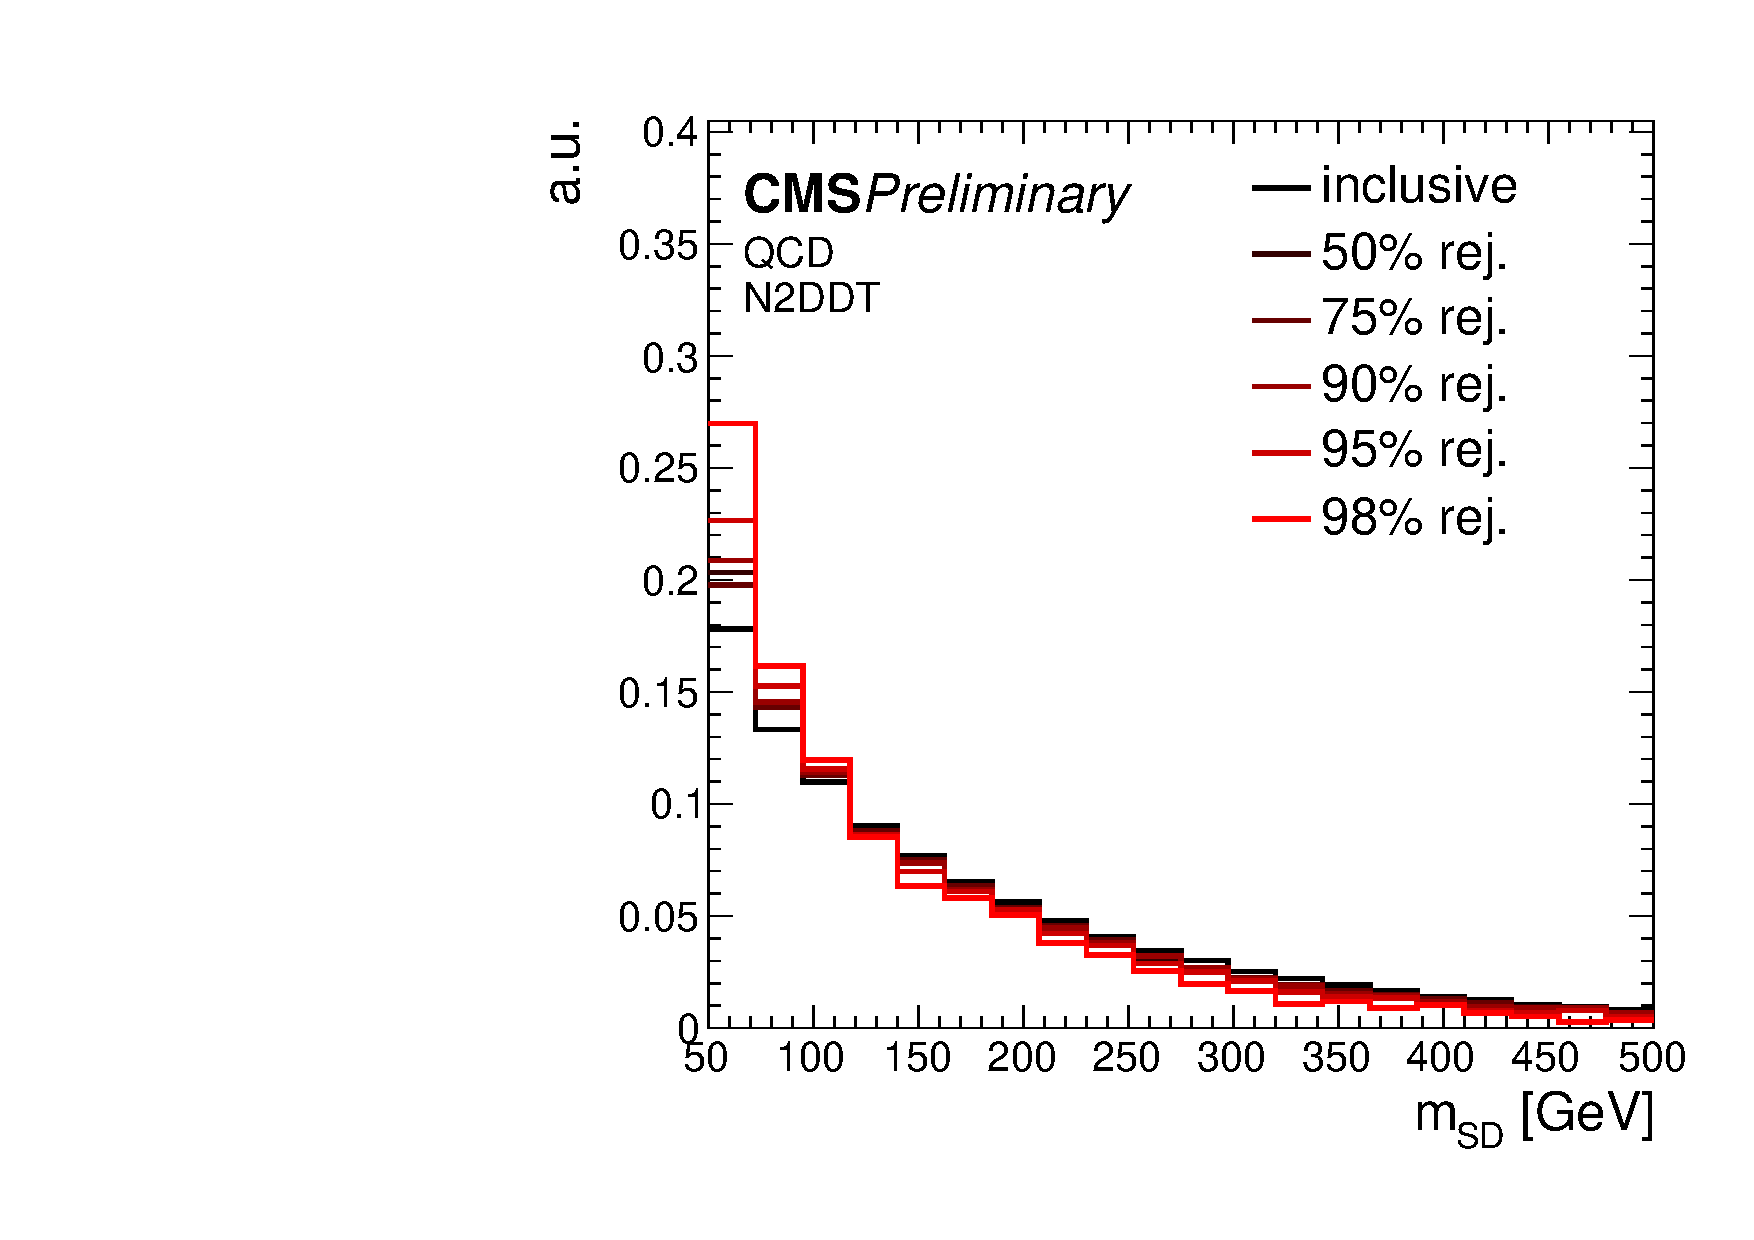
\includegraphics[width=0.475\textwidth]{figures/higgstagging/QCDN2DDT_mSD.pdf}\\
  \caption{Tagging kinematics: shown is the dependence of the soft drop mass on the $N_2$, $\tau_{21}^\text{SD}$, and N2DDT cut. The mass sculpting is pronounced for the variables before decorrelation, while N2DDT shows practically no mass sculpting.}
  \label{fig:taggingkinematics}
\end{figure}


Because we want to preserve a smoothly falling jet mass distribution as a function of \pt, it is natural to determine a substructure variable's stability as a function of the QCD scaling variable $\rho=log(m_{\text{SD}}^2/\pt^2)$.
Since the QCD (quark or gluon-initated) jet mass scales with \pt, decorrelating a given substructure variable as a function of $\rho$ and \pt is a well-bounded procedure.

\begin{figure}
  \centering
  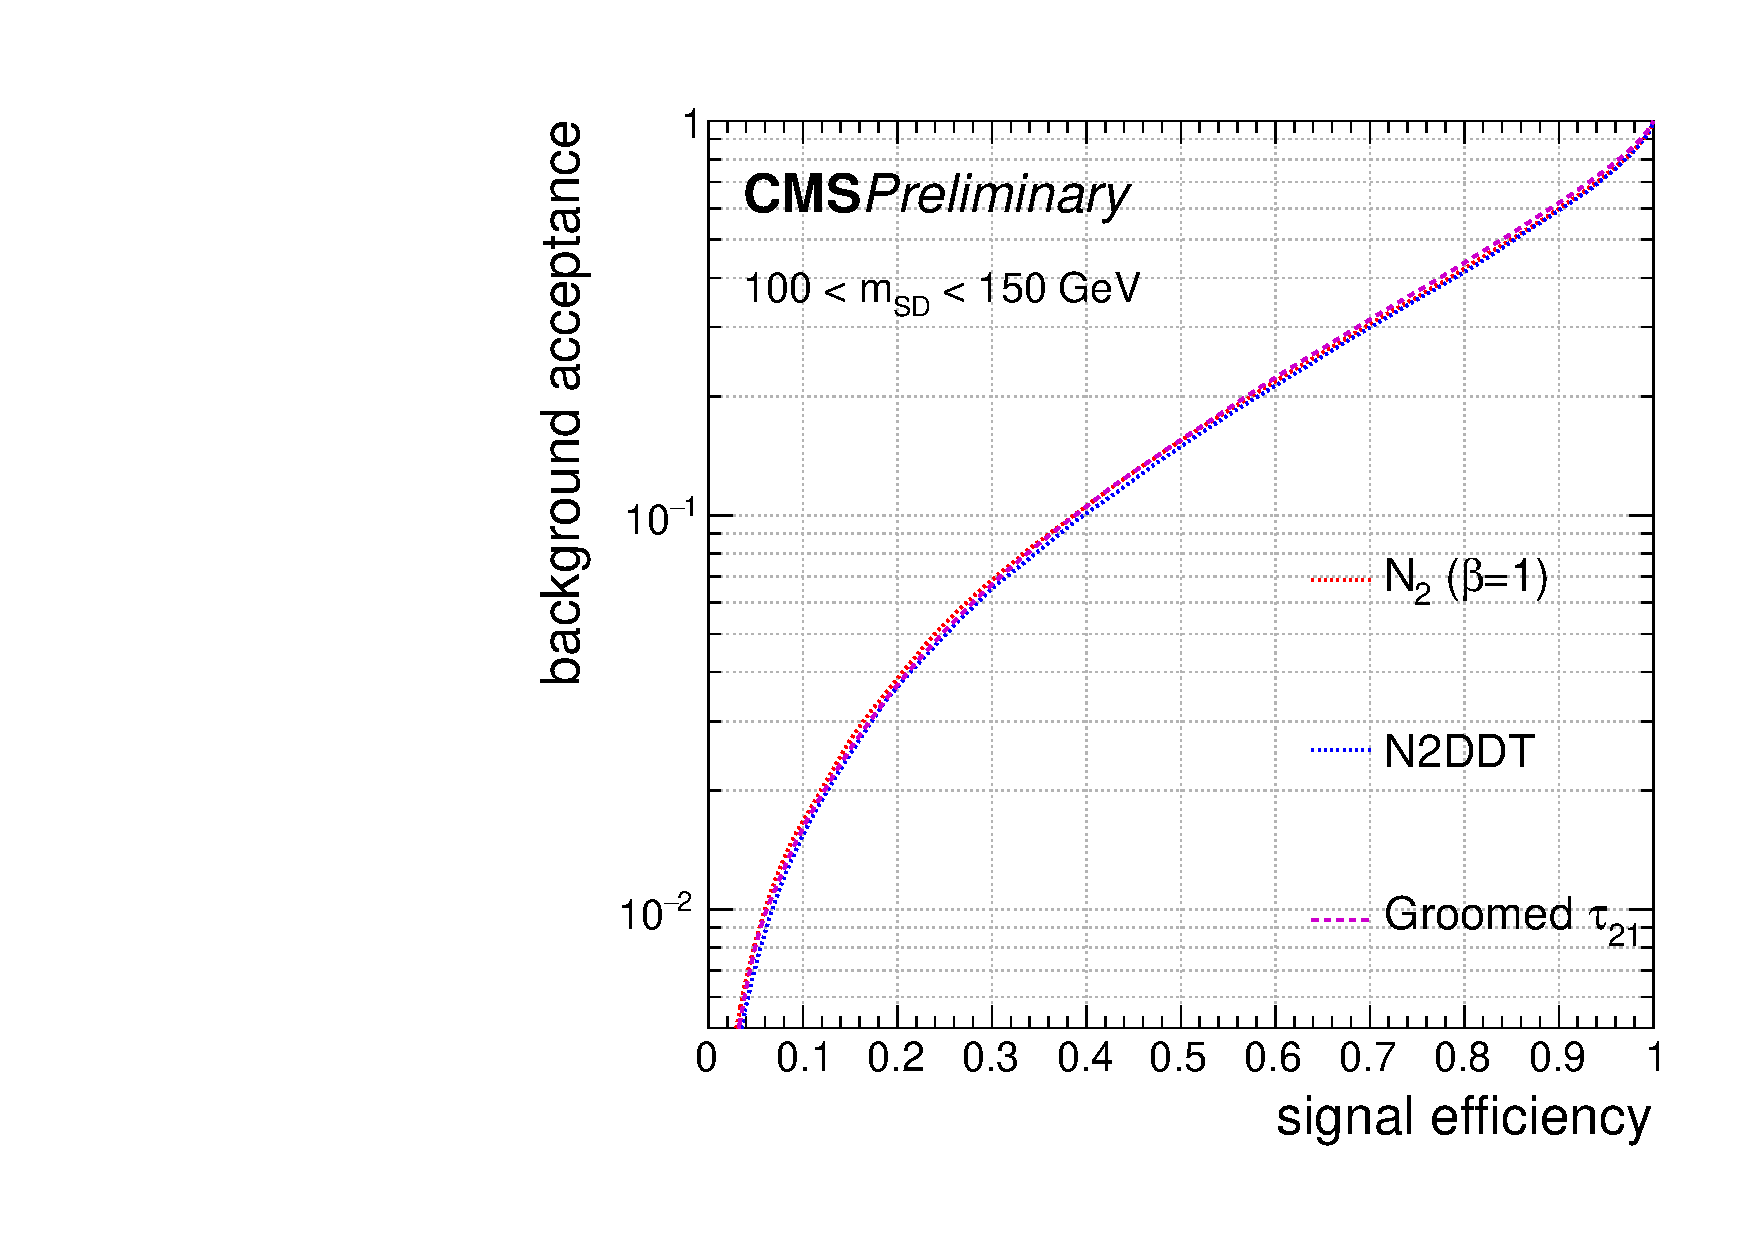
\includegraphics[width=0.475\textwidth]{figures/higgstagging/massCut_roc.pdf}
  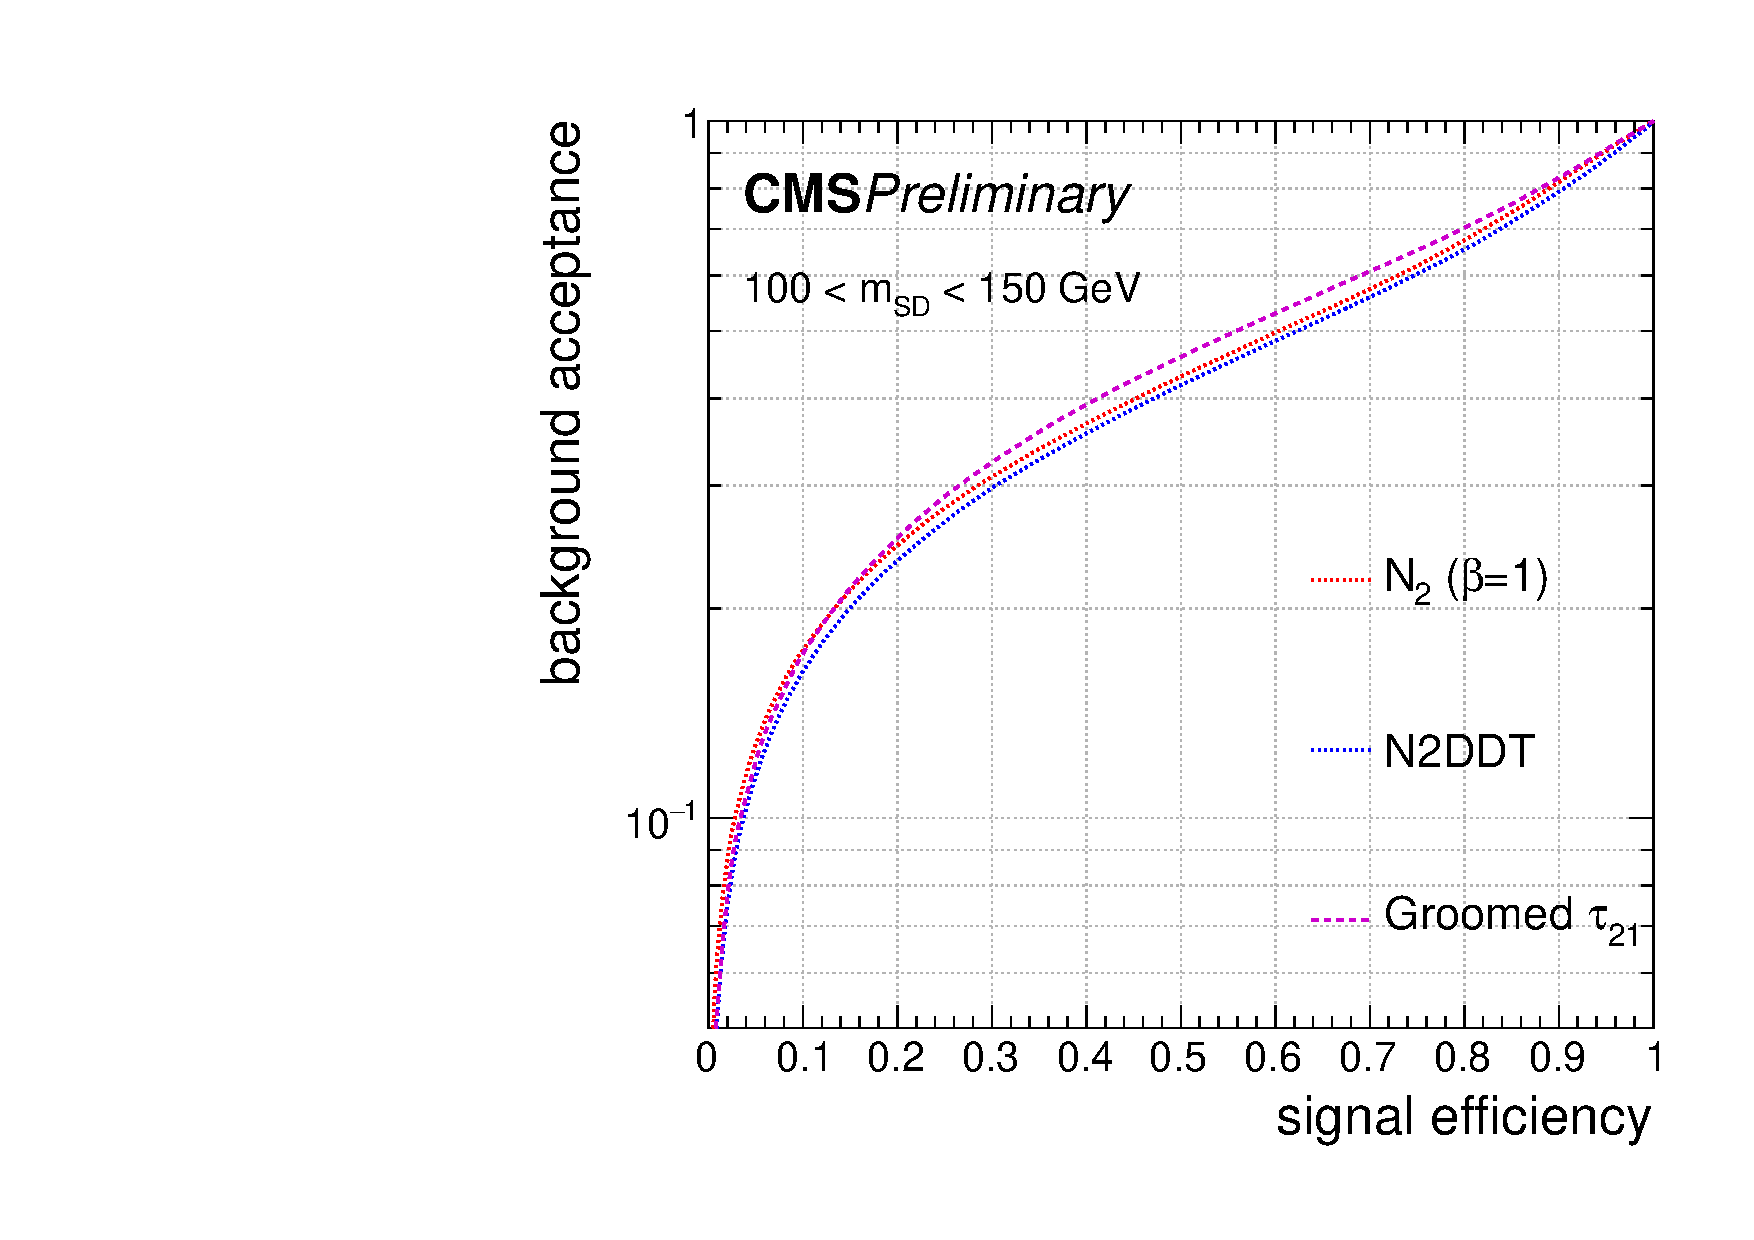
\includegraphics[width=0.475\textwidth]{figures/higgstagging/massCut_roc_top.pdf}\\
  \caption{ROC curves for the $N_2$ and $N$-subjettiness variables. Left: rejection of QCD jets. Right: rejection of top jets. While both $N_2$ and $\tau_{21}$ have similar power to discriminate Higgs jets from QCD jets, $N_2$ does a better job in rejecting fat jets originating from a boosted hadronic top quark decay.}
  \label{fig:n2rocs}
\end{figure}


\begin{figure}
  \centering
  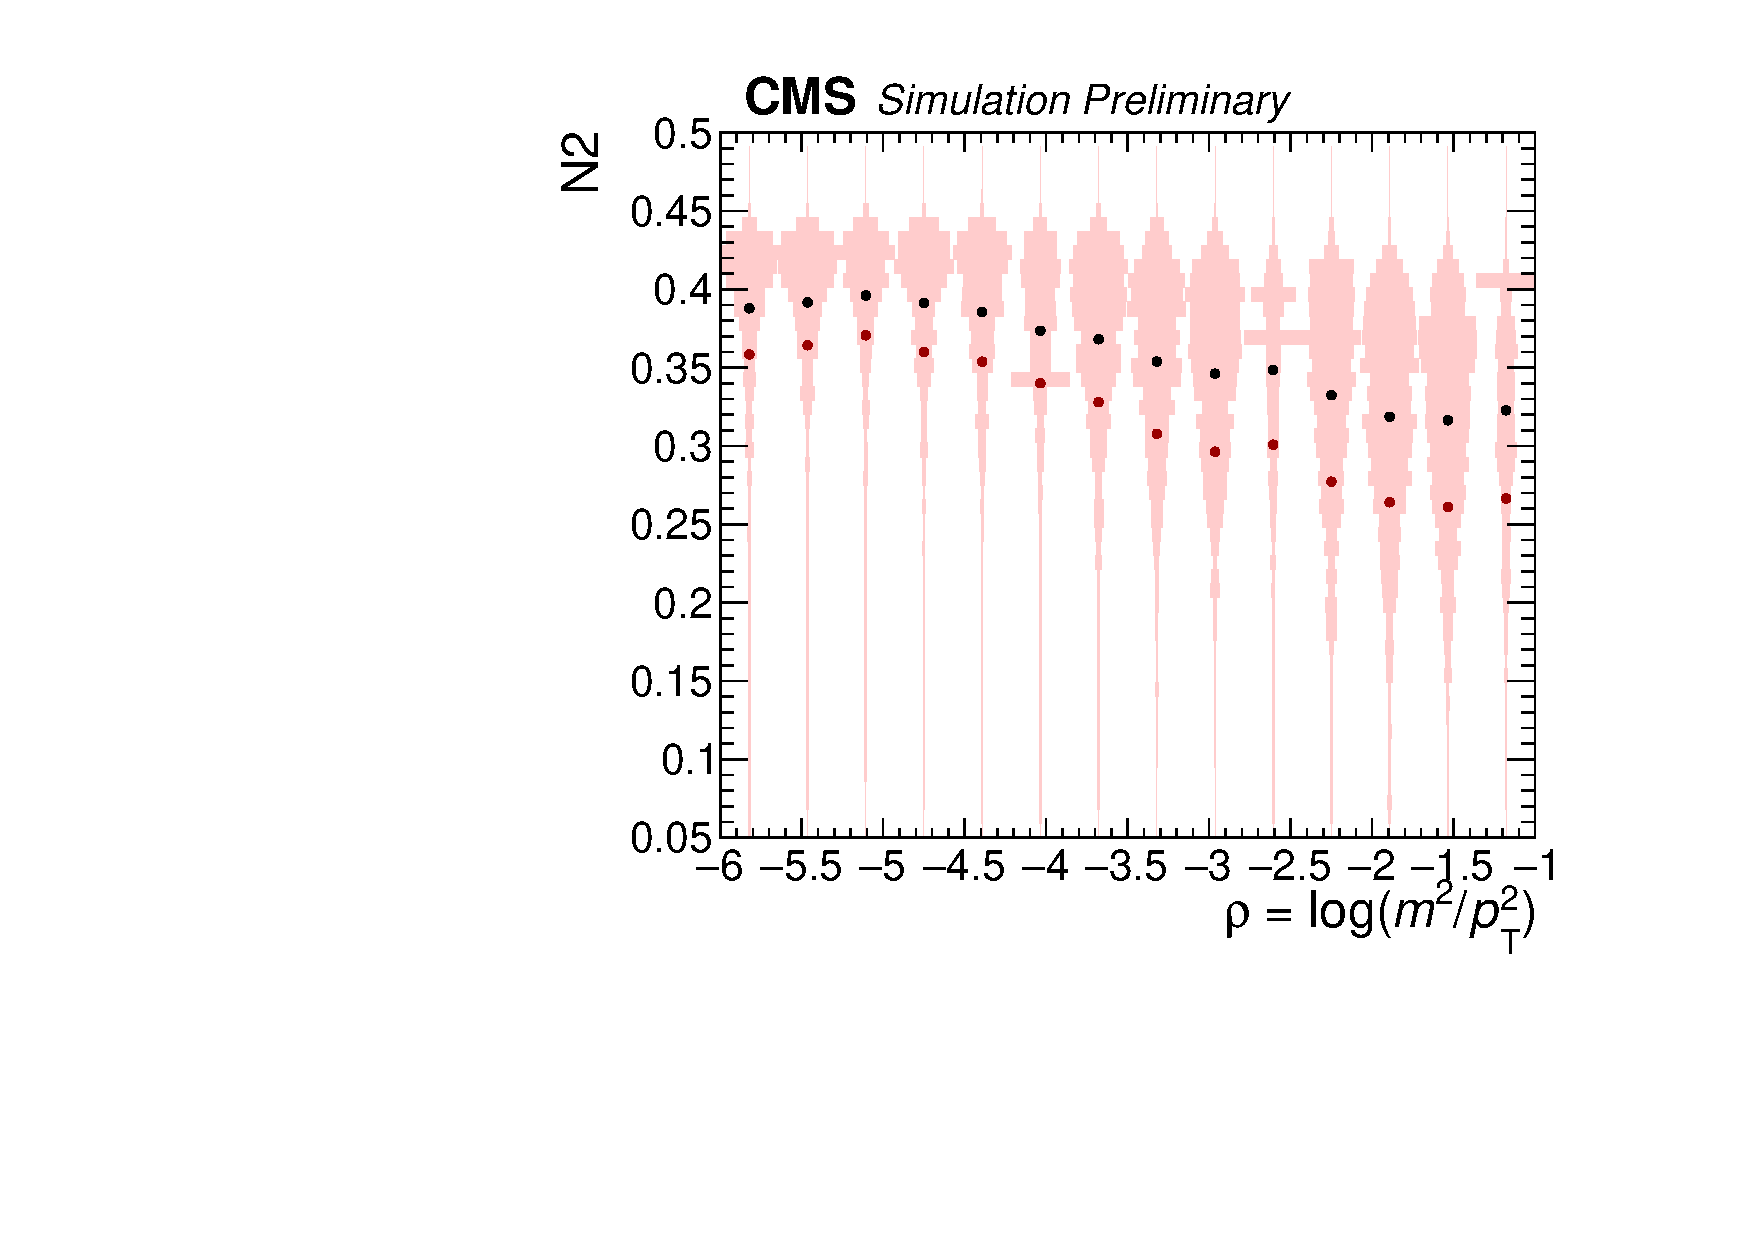
\includegraphics[width=0.38\textwidth]{figures/higgstagging/n2ddt/h2s_n2Vrho0.pdf}\put(-135,25){200-400\GeV}
  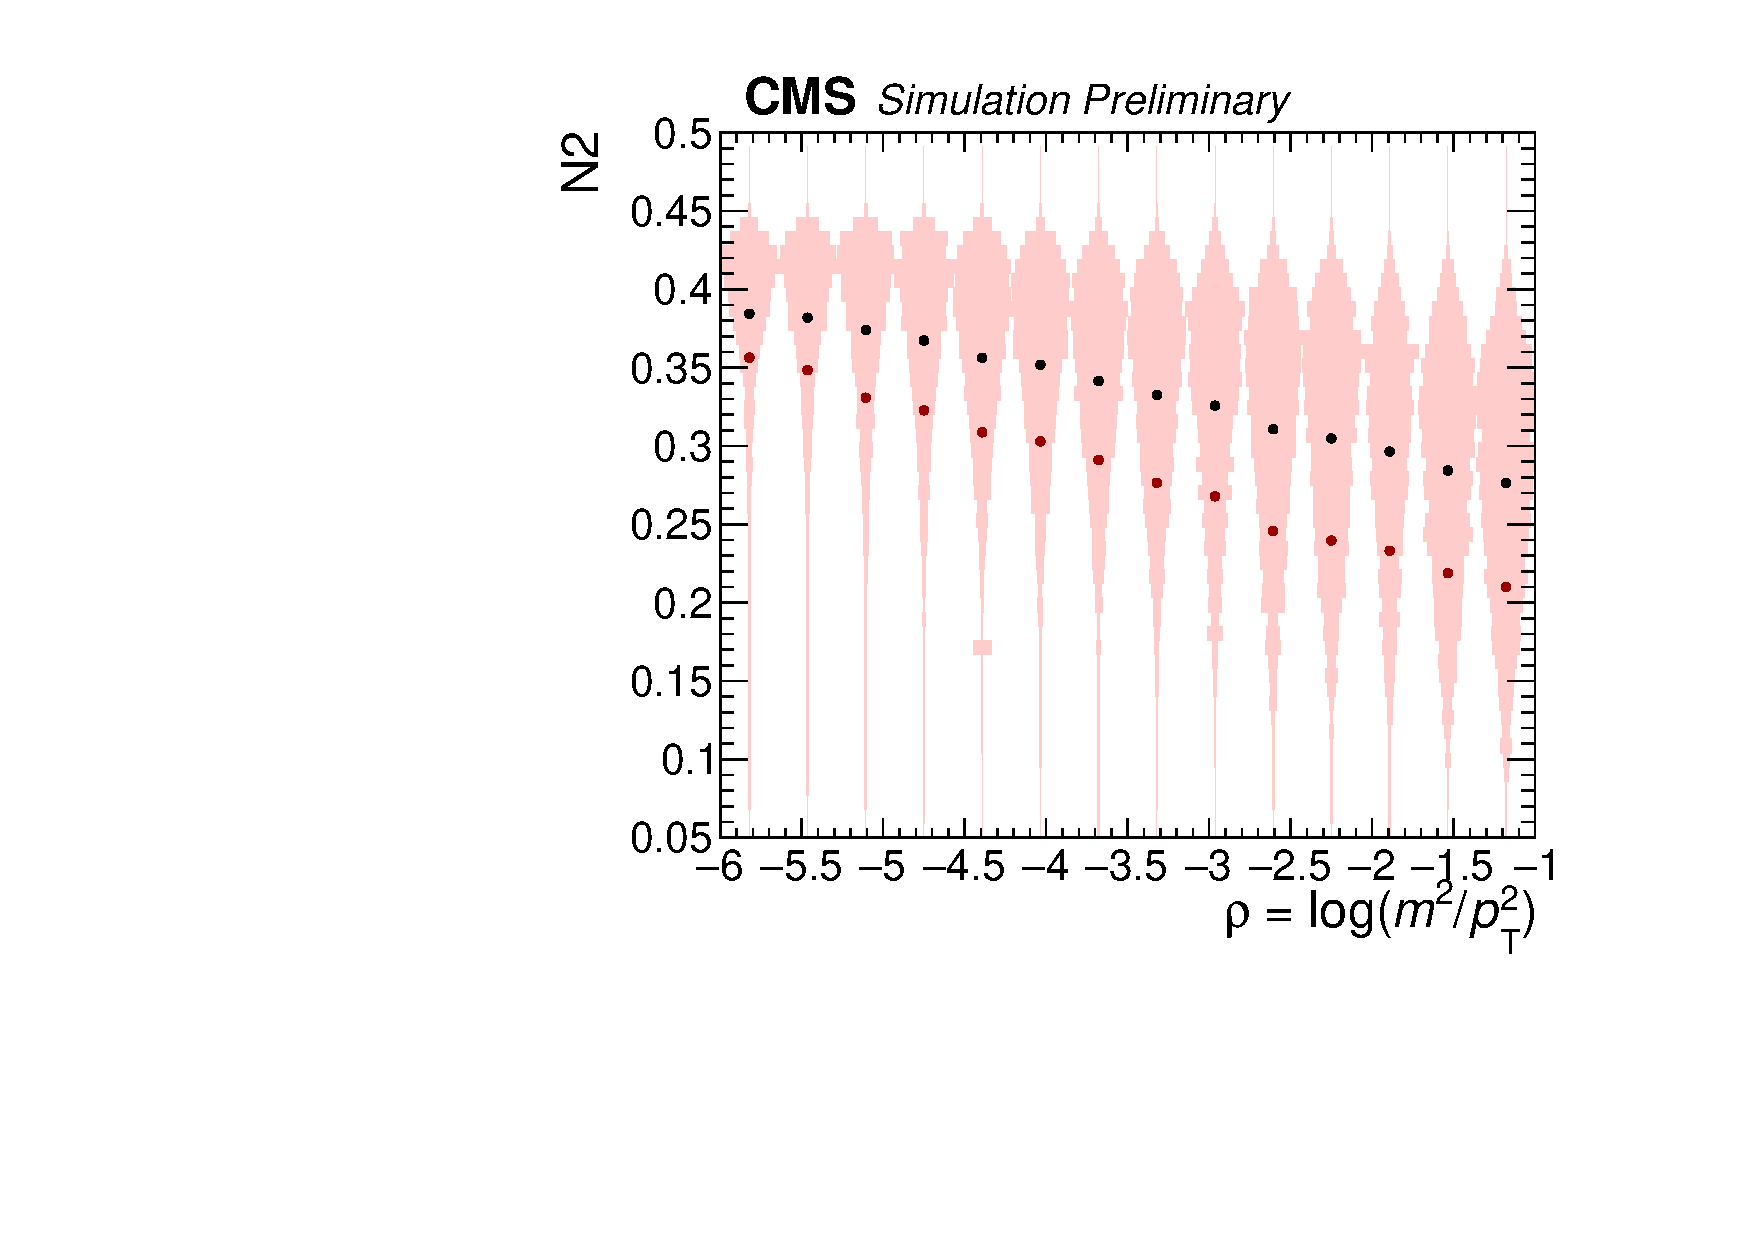
\includegraphics[width=0.38\textwidth]{figures/higgstagging/n2ddt/h2s_n2Vrho1.pdf}\put(-135,25){400-600\GeV}\\
  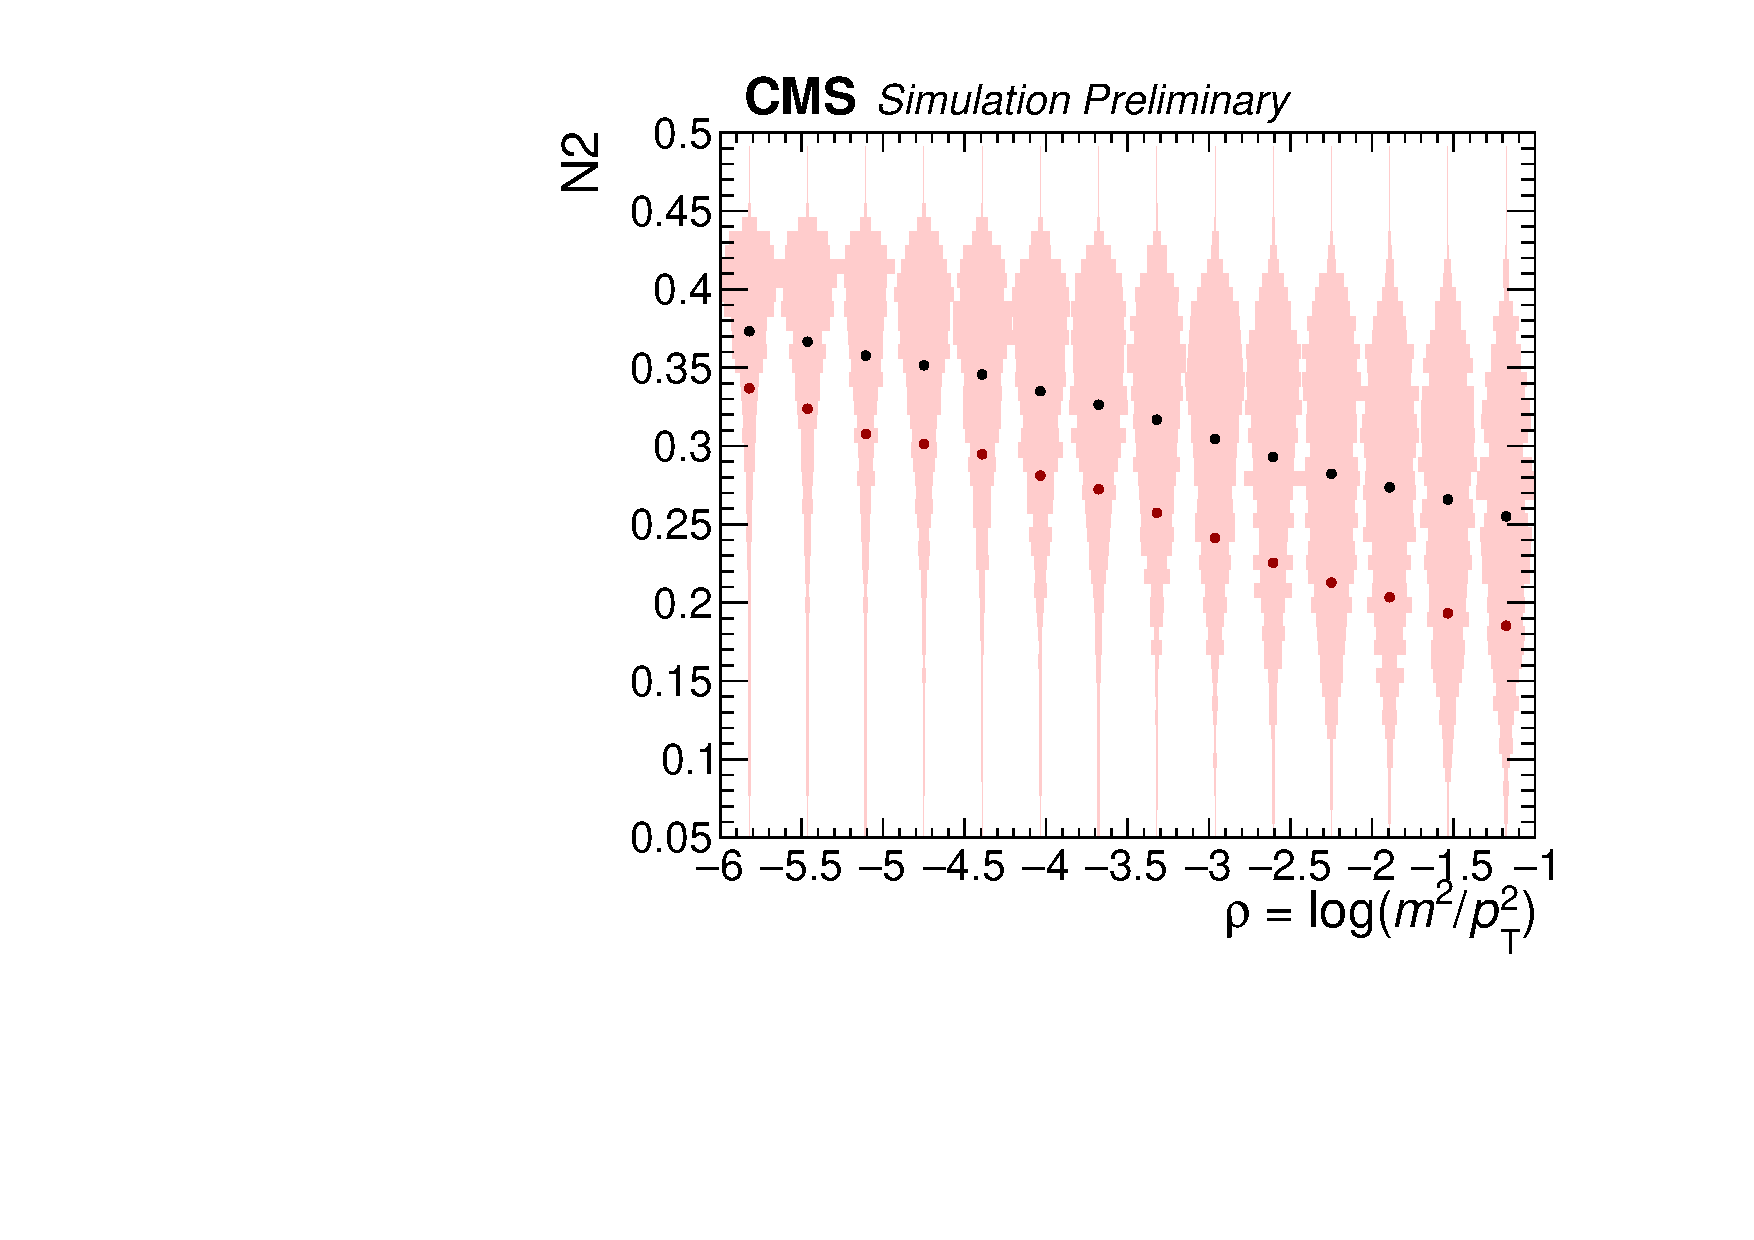
\includegraphics[width=0.38\textwidth]{figures/higgstagging/n2ddt/h2s_n2Vrho2.pdf}\put(-135,25){600-800\GeV}
  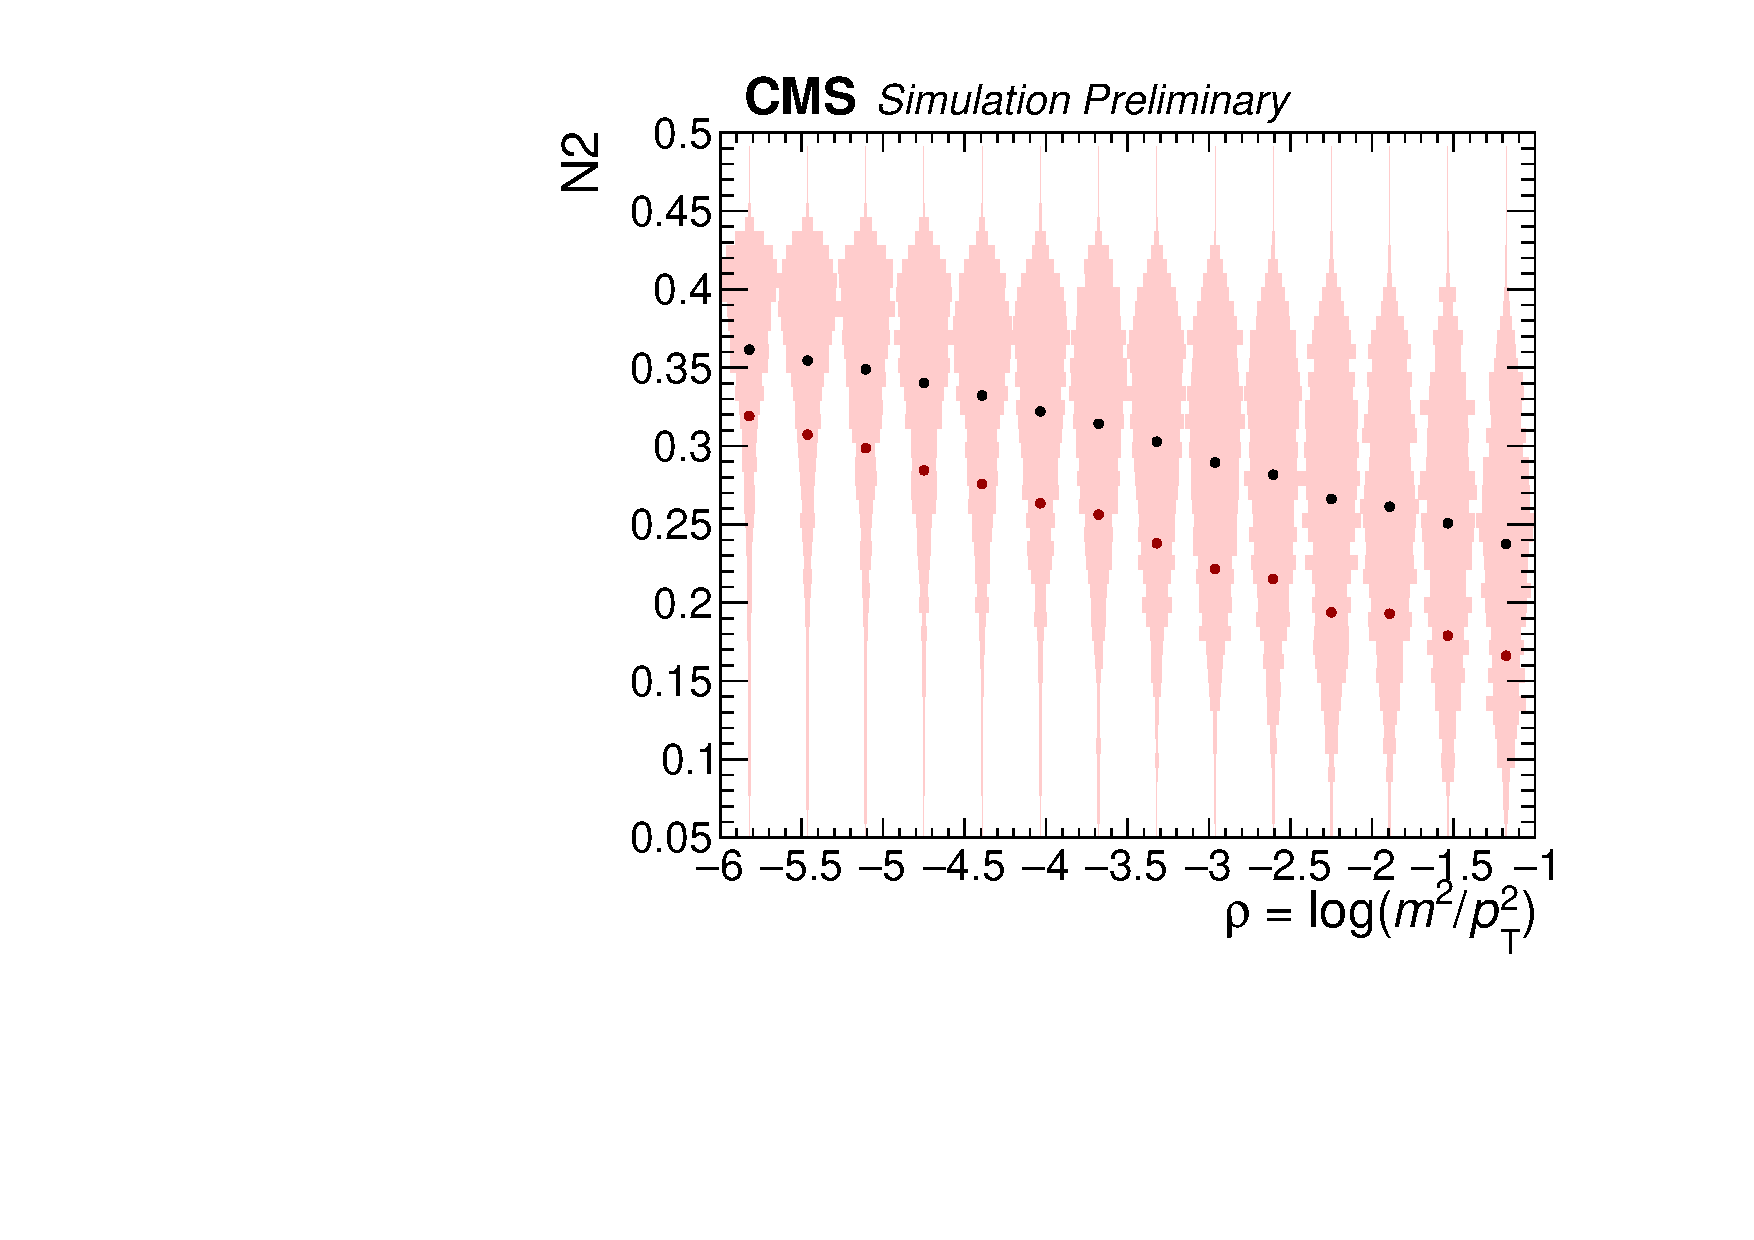
\includegraphics[width=0.38\textwidth]{figures/higgstagging/n2ddt/h2s_n2Vrho3.pdf}\put(-135,25){800-1000\GeV}\\
  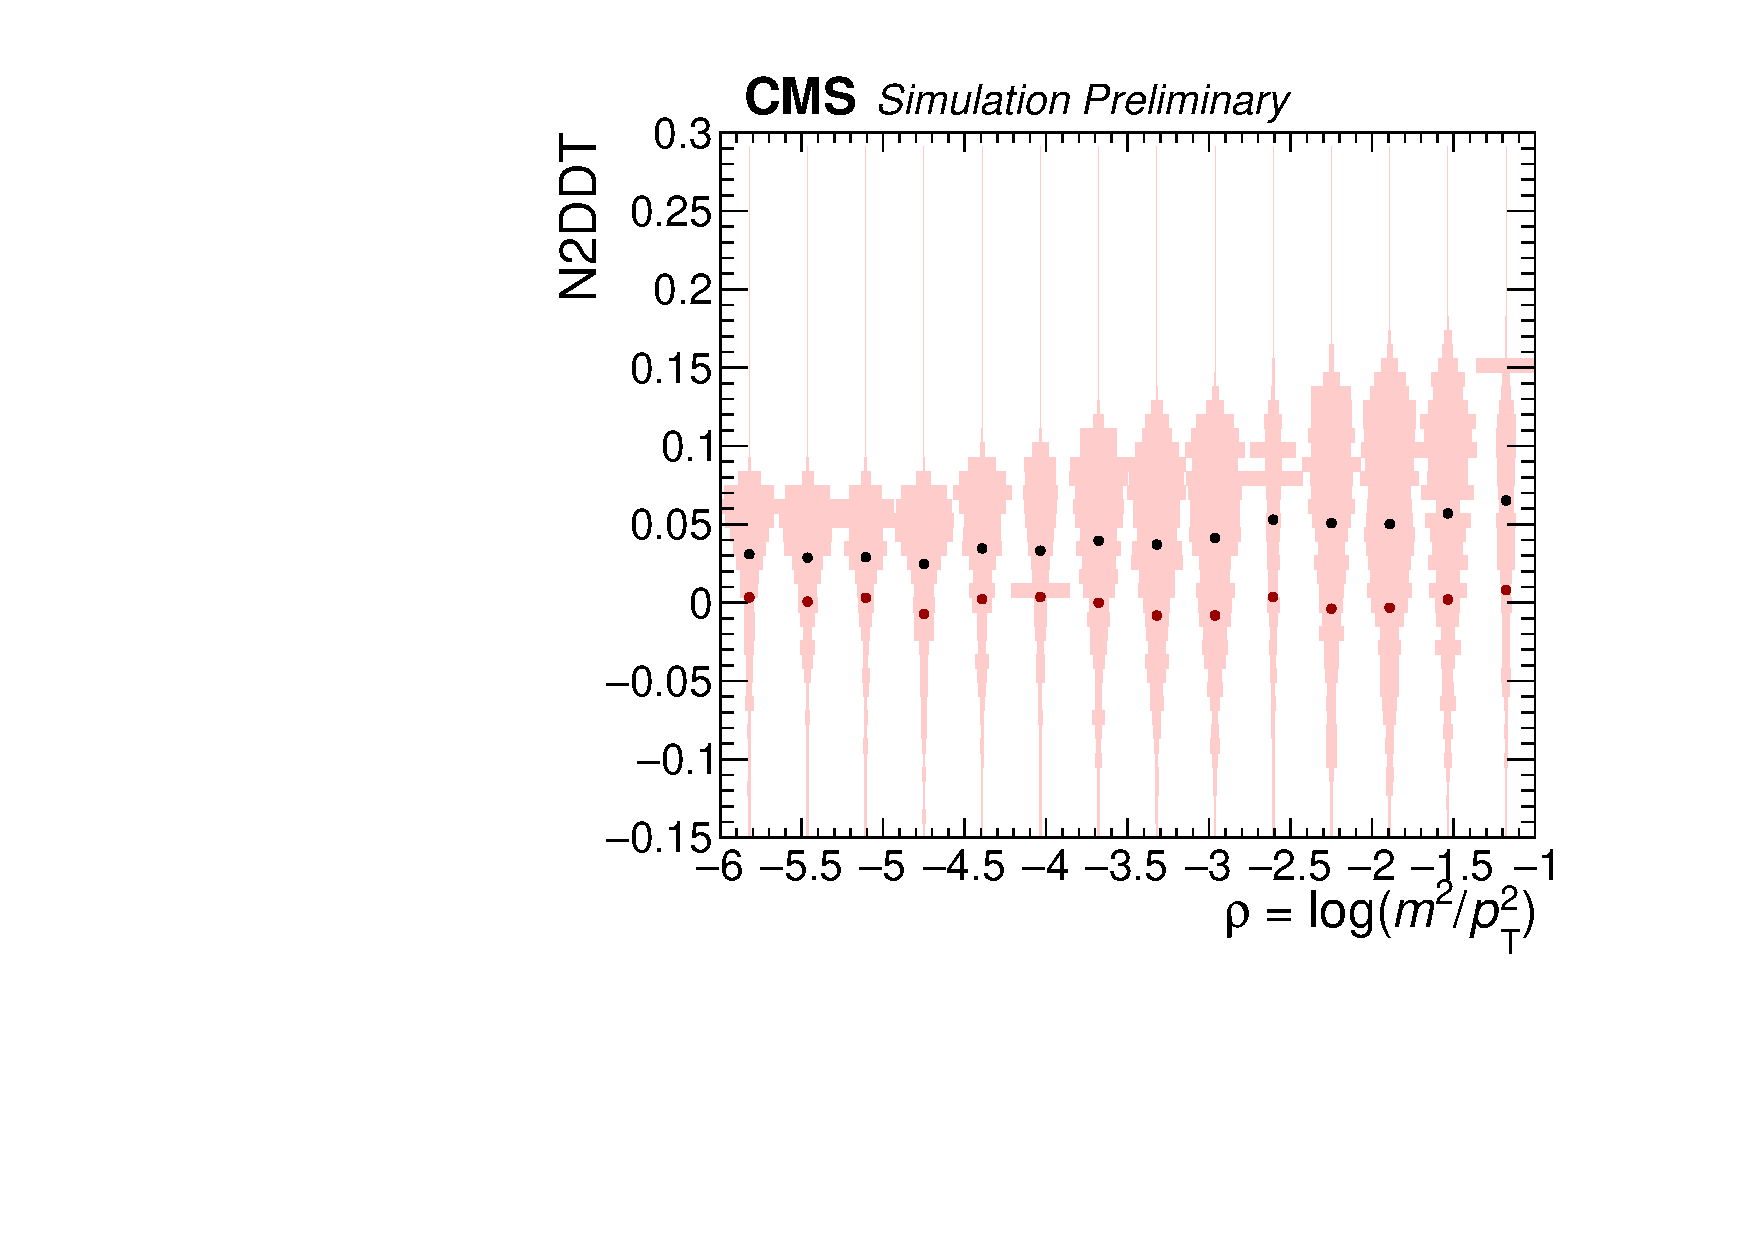
\includegraphics[width=0.38\textwidth]{figures/higgstagging/n2ddt/h2s_n2ddtVrho0.pdf}\put(-135,25){200-400\GeV}
  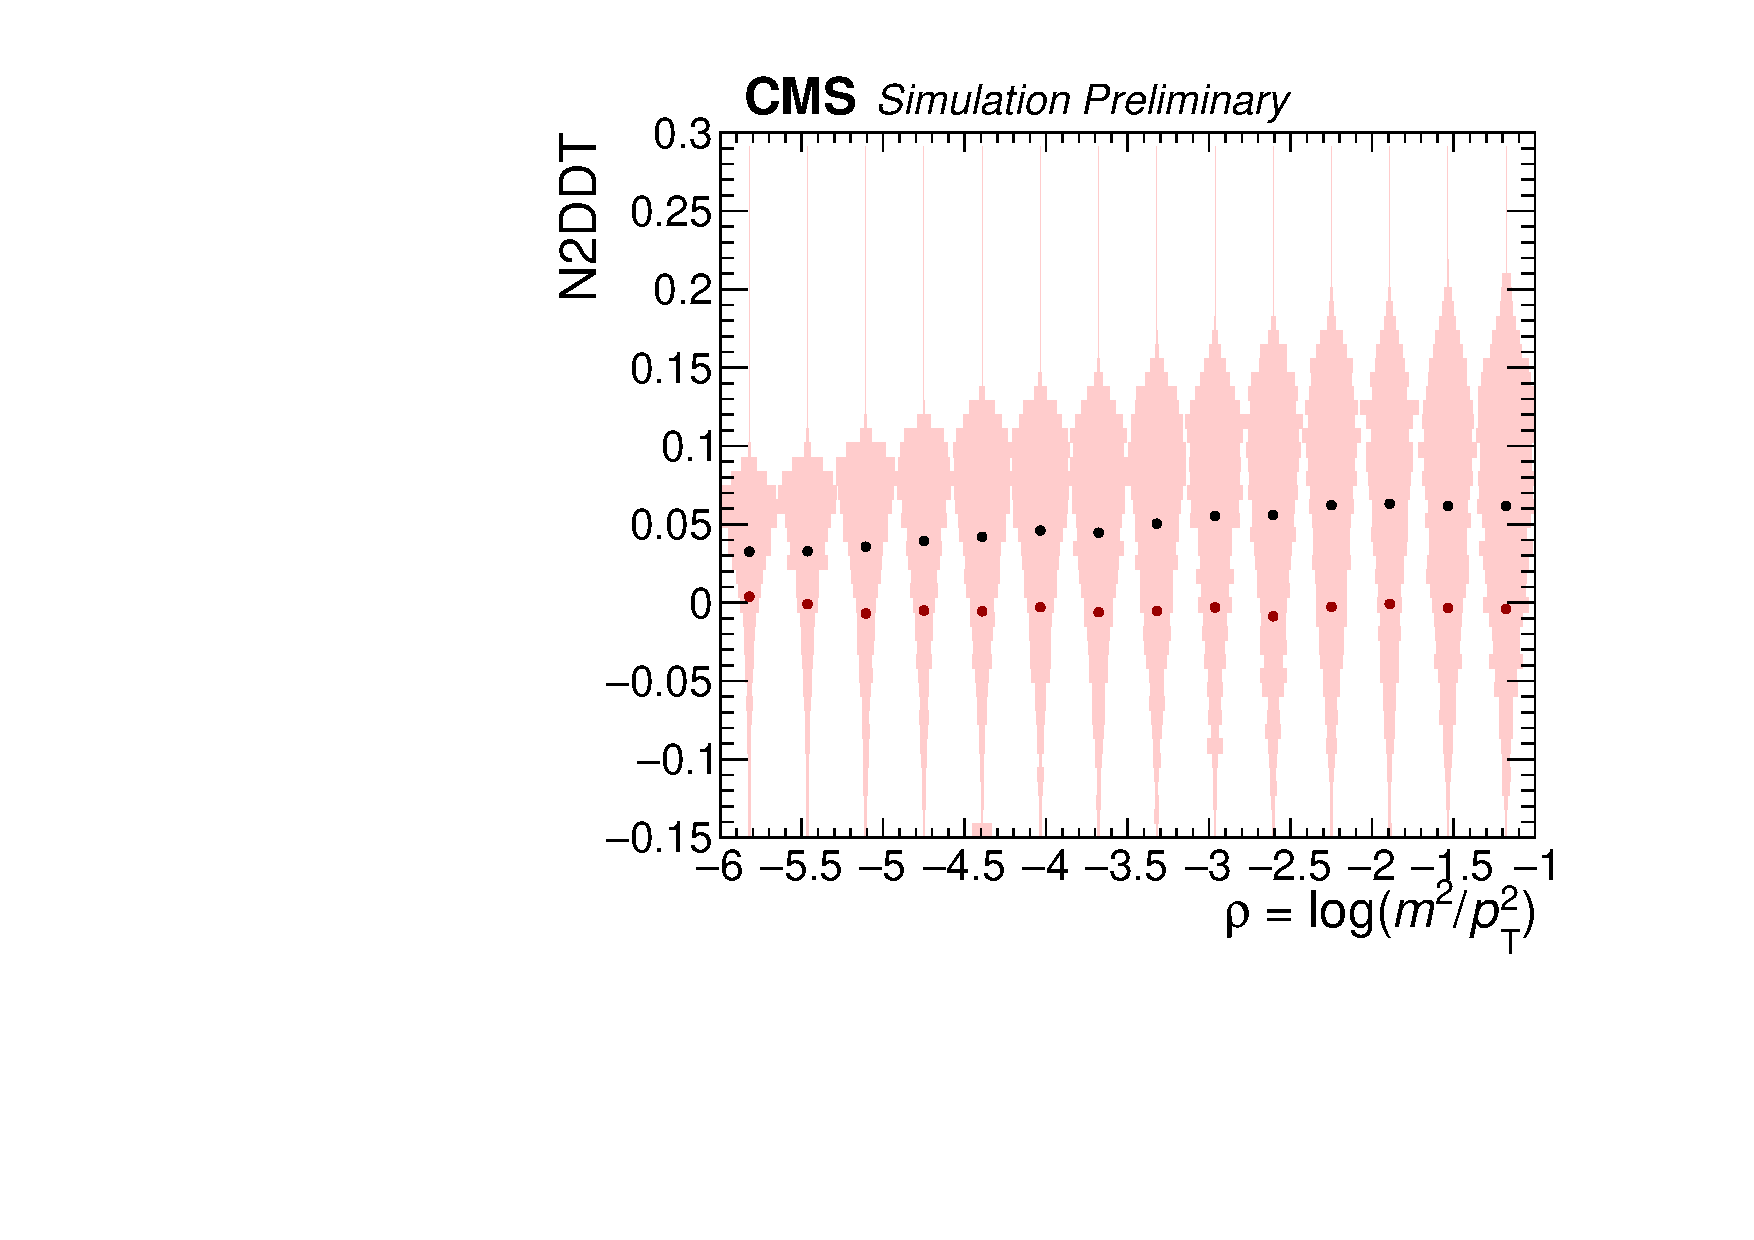
\includegraphics[width=0.38\textwidth]{figures/higgstagging/n2ddt/h2s_n2ddtVrho1.pdf}\put(-135,25){400-600\GeV}\\
  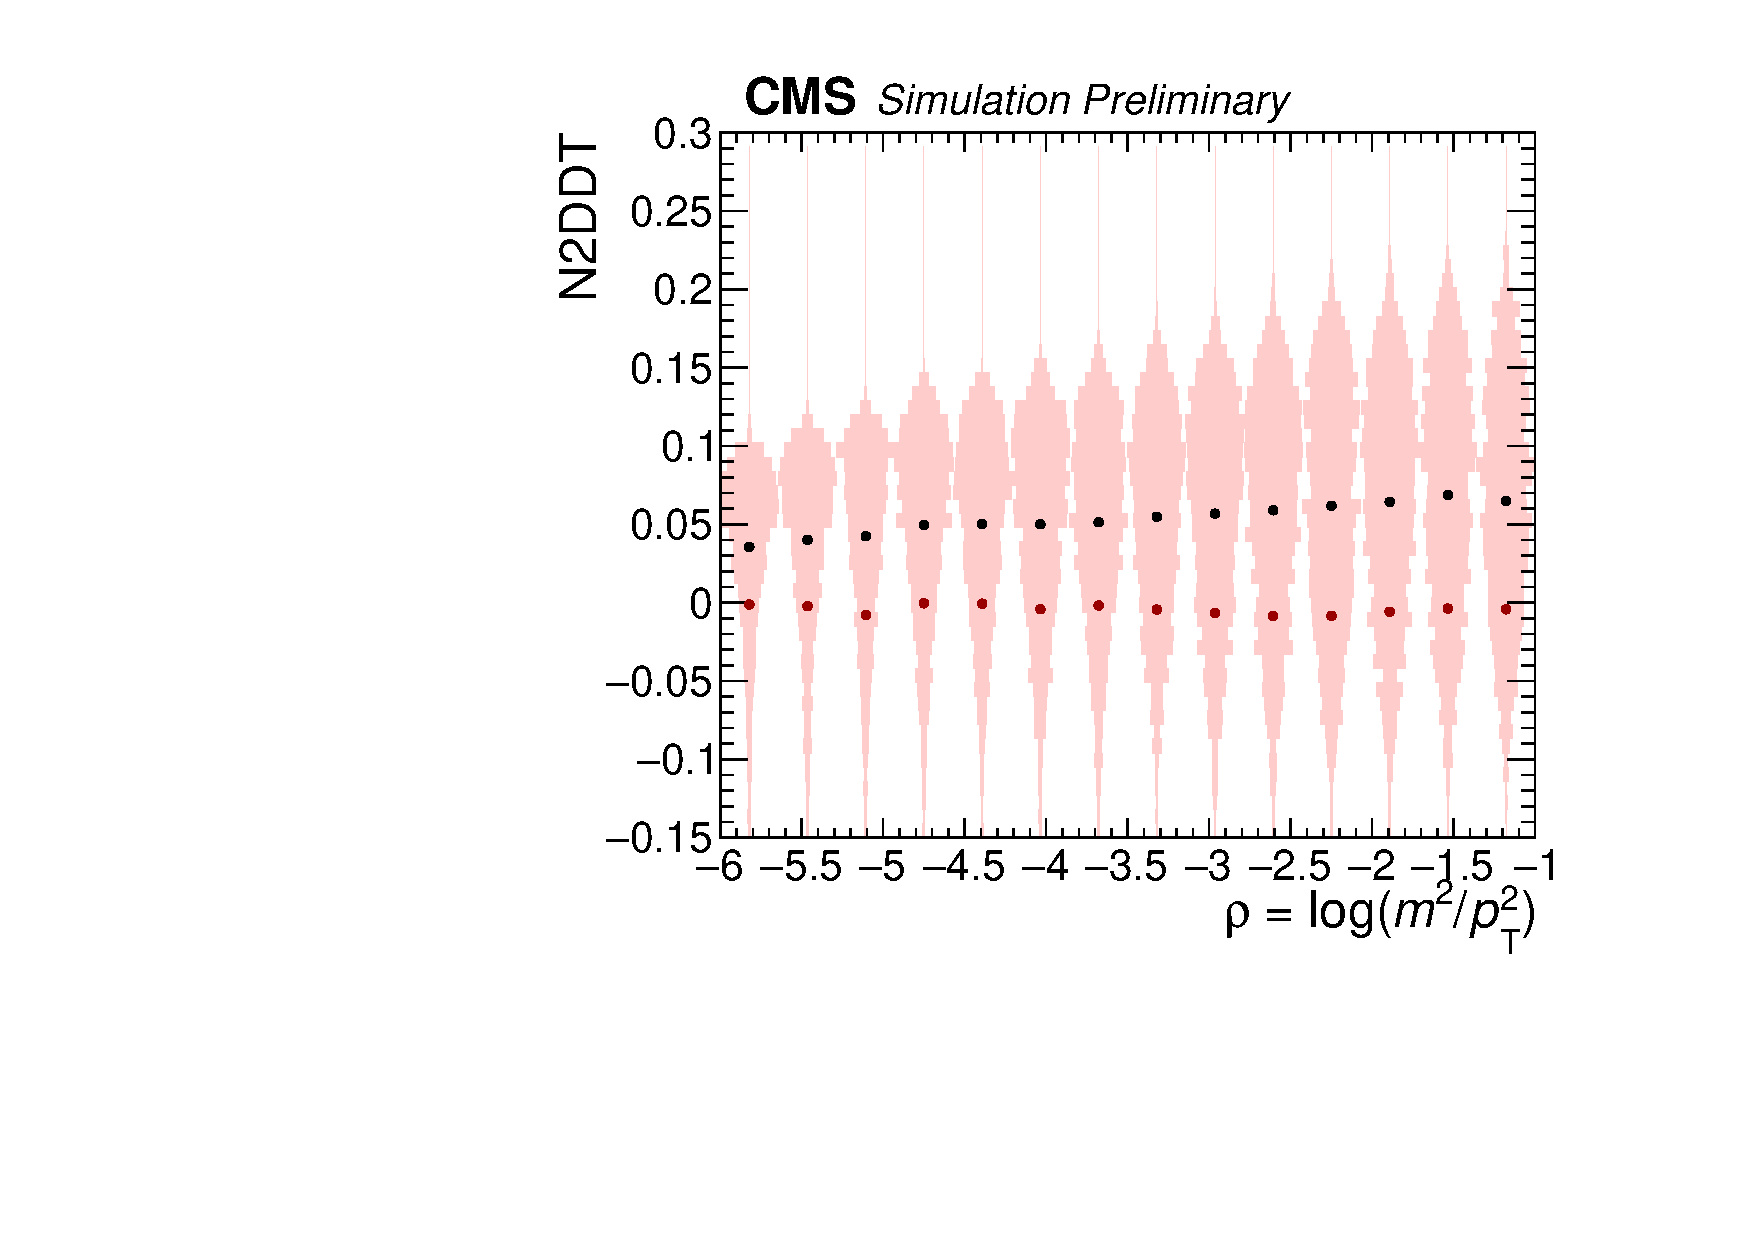
\includegraphics[width=0.38\textwidth]{figures/higgstagging/n2ddt/h2s_n2ddtVrho2.pdf}\put(-135,25){600-800\GeV}
  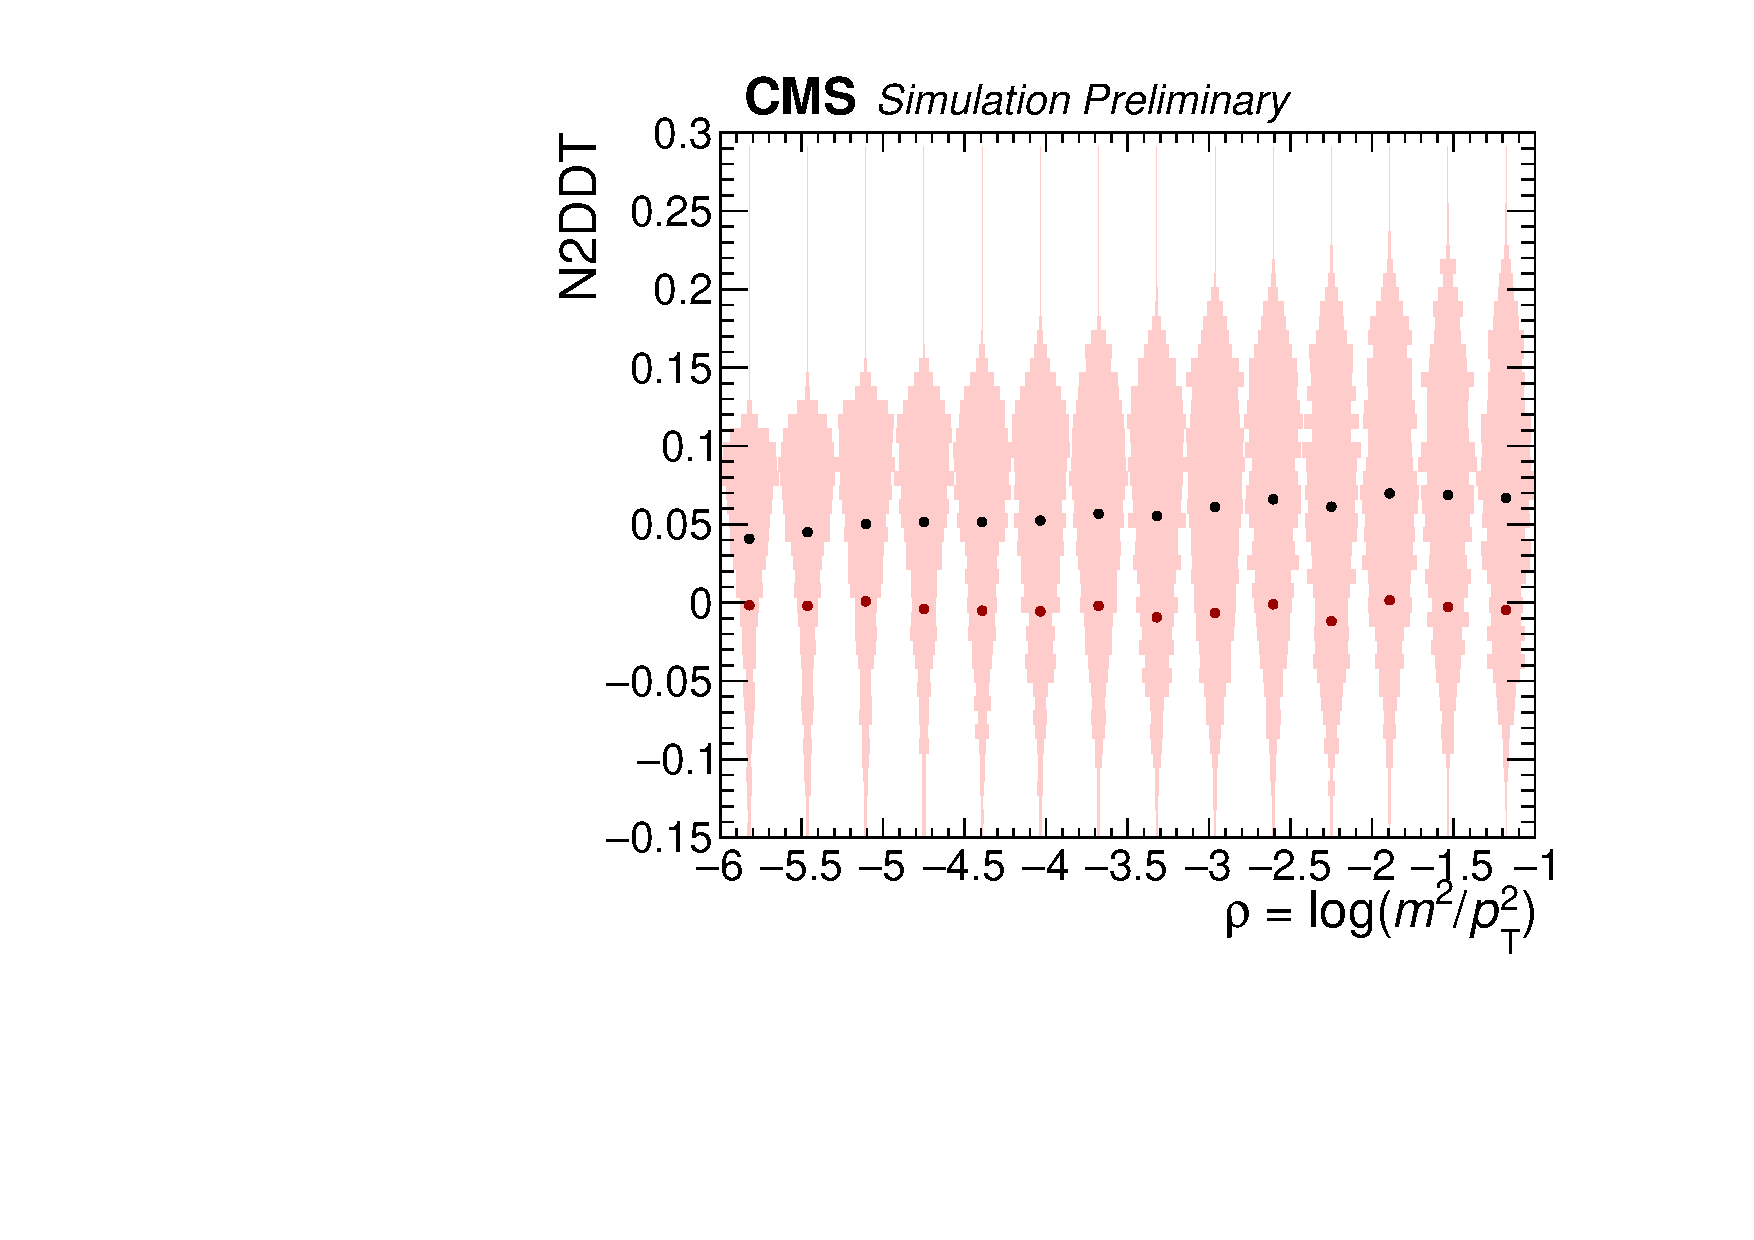
\includegraphics[width=0.38\textwidth]{figures/higgstagging/n2ddt/h2s_n2ddtVrho3.pdf}\put(-135,25){800-1000\GeV}\\
  \caption{Kinematic dependence of $N_2$ and $N_2^\text{DDT}$ as a function of $\rho$ in different \pt bins.}
  \label{fig:violins}
\end{figure}




The decorrelation procedure will be applied at the 20\% background efficiency point, which corresponds to a signal efficiency of roughly 50\%.
This choice of background (or, equivalently, signal) efficiency has been made weighing a good $S/B$ ratio against retaining high enough event yields for the data-driven estimation of the background processes. In particular, going lower in background efficiency brings in large statistical uncertainties on the transfer factors in the simultaneous fit from which we derive upper limits, while a scenario with a significantly higher signal efficiency suffers from large background contaminations degrading the search sensitivity.
The top four plots of Figure~\ref{fig:violins} show the 2D correlations of $\rho$ with $N_2^\text{DDT}$ shown in ``violin'' style for four different \pt bins.
The black dots represent the 50\% background efficiency point for cutting on $N_2^\text{DDT}$ while the red points represent other
the 20\% background efficiency scenario.
%The inflection in the distribution around $\rho = 2$ comes from finite jet size effects which represents a natural limit to the mass of a QCD jet for a given \pt.
Below $\rho = 6$ we enter the non-peturbative regime of the soft drop mass calculation and therefore cut-off the mapping there.
For this analysis a transformation which fixes the background efficiency at 20\% is performed. The efficiency is chosen in agreement with other analyses that use $N_2$ as Higgs-tagging variable (usually around 25\%), tuned to optimize the sensitivity to the mono-Higgs signal.  
The 2D map in $\{\rho,\pt\}$ space which transforms $N_2 \rightarrow N_2^\text{DDT}$ is shown in Fig.~\ref{fig:transmap_20percent}.
Therefore, the transformation is defined as:
\begin{equation}
N_2^\text{DDT} = N_2 - N_2(\text{cut at 20\%})
\end{equation}

\begin{figure}
  \centering
  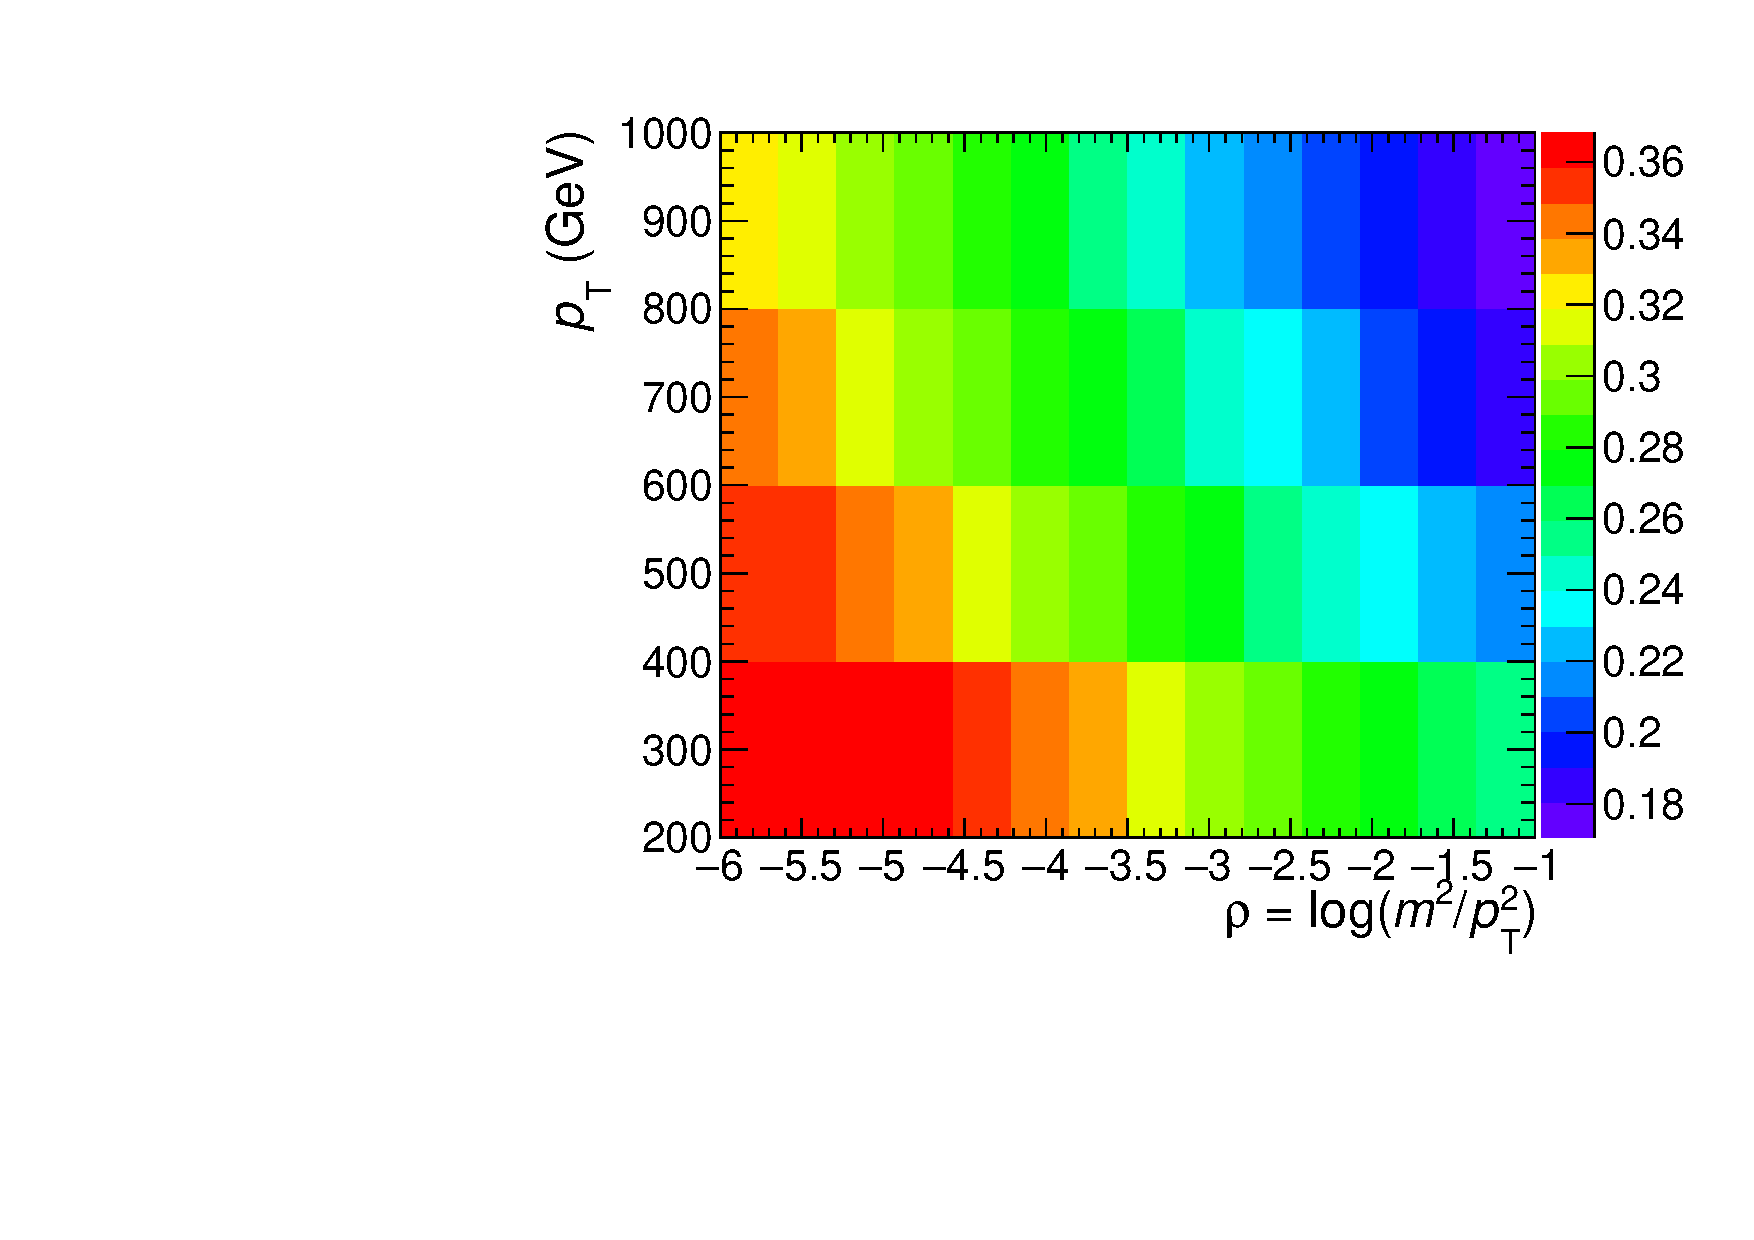
\includegraphics[width=0.475\textwidth]{figures/higgstagging/n2ddt/h2ddt.pdf}
  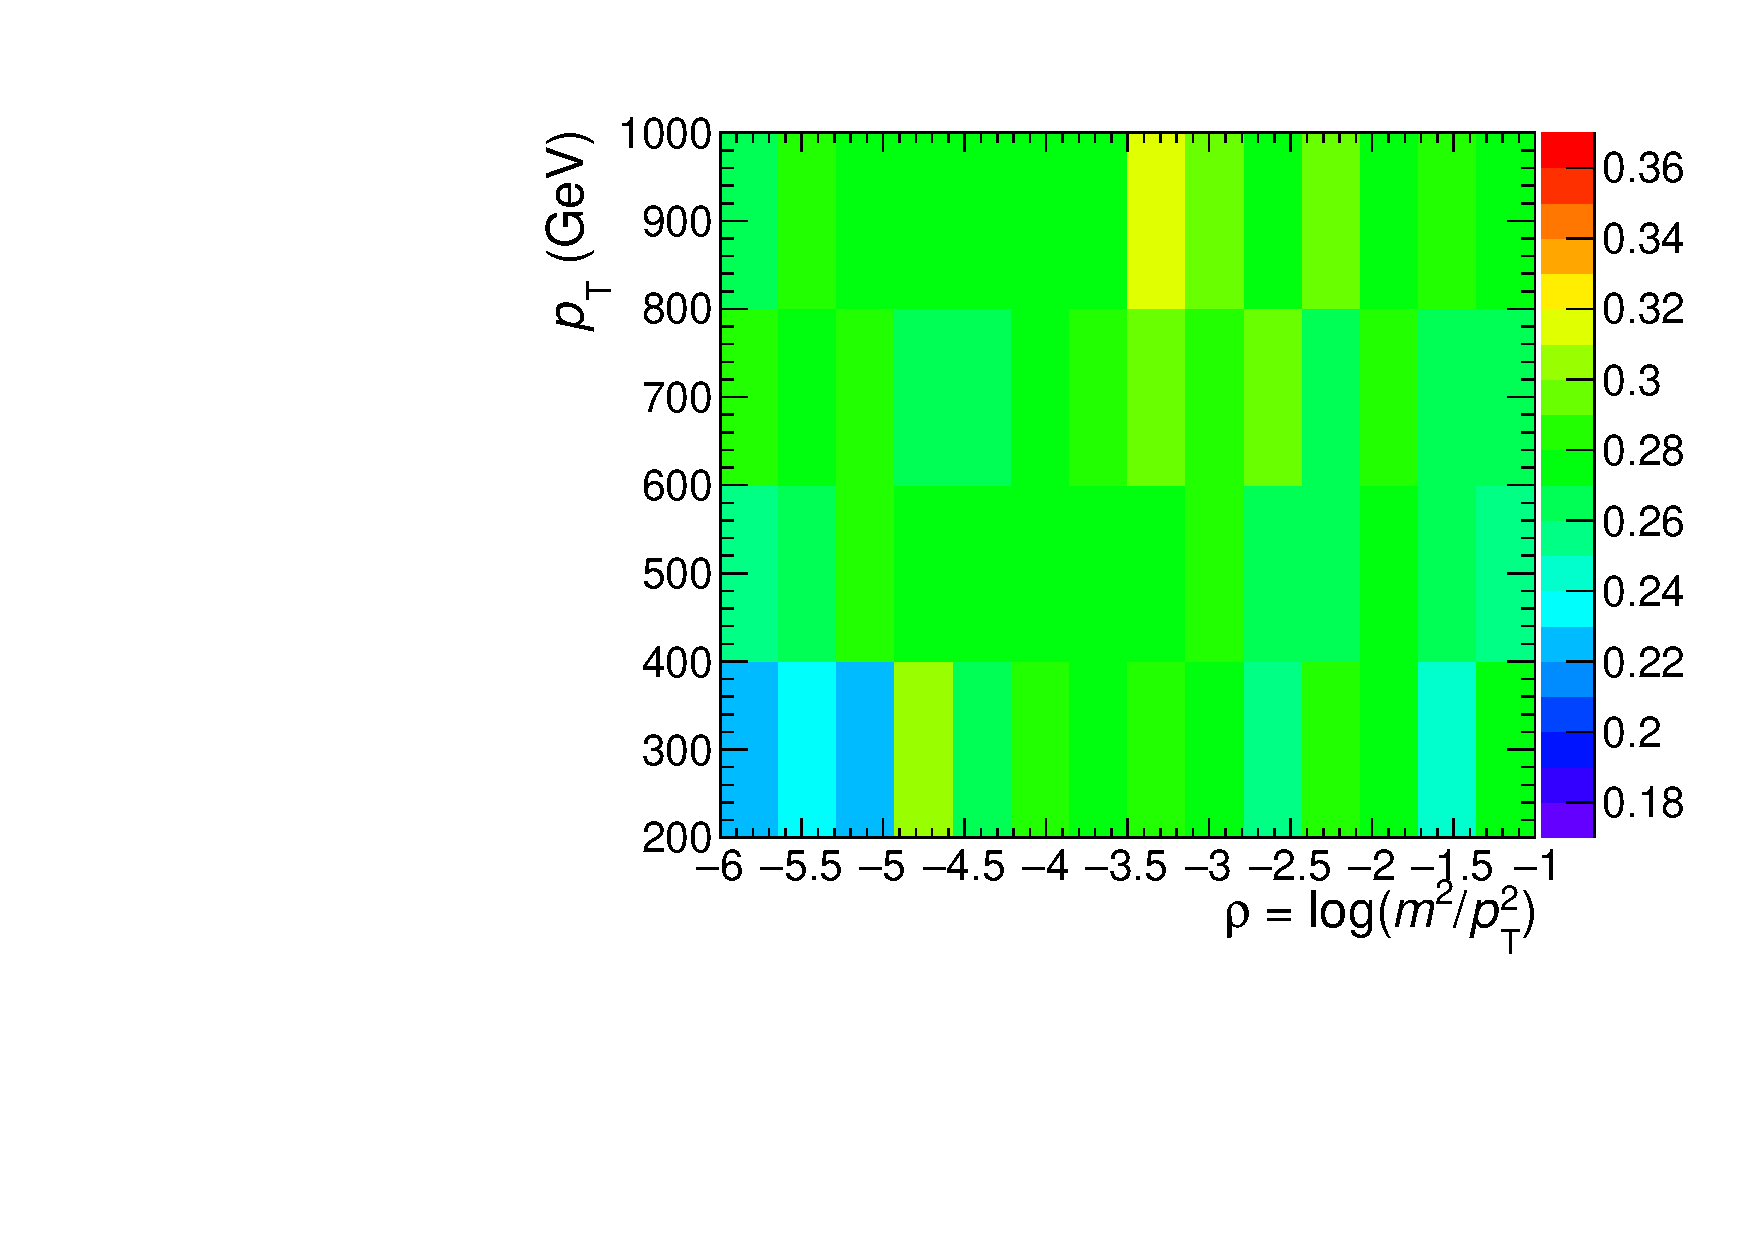
\includegraphics[width=0.475\textwidth]{figures/higgstagging/n2ddt/h2_rhoVpt_pafa.pdf}\\
  \caption{Left: transformation map of $N_2\rightarrow N_2^{\text{DDT}}$. Right: the $z$-axis gives the ``pass-over-fail'' ratio when cutting on $N_2^\text{DDT}<0$. By construction, this ratio is equal to $0.2/0.8\sim0.25$. This is found across all bins in $\rho$ and $\pt$.}
  \label{fig:transmap_20percent}
\end{figure}

The ``pass-over-fail'' in QCD background is also shown in Fig.~\ref{fig:transmap_20percent}. We observe tagging (in)efficiencies that are flat across the entire phase space. 


Once a cut on this variable is applied to both MC and data, different residual tagging efficiencies have to be accounted for by means of a scale factor. This scale factor is measured in semileptonic \ttbar events, where the top quark is not fully merged, but one is instead left with a fat jet stemming from a hadronically decaying boosted W boson~\cite{CMS_AN_2016-219}.


%%%
%In order to extract the W-tagging scale factors, the W-tagging efficiency of a pure W-jet sample must be estimated in data and simulation. This is done by validating the shapes of the real, merged Ws and the pure combinatorial background for the pass and fail W-tagged events in the \ttbar simulated sample. The \ttbar sample is divided into the combinatorial background and the real, merged Ws at generator level, matching the CA15 jet in a cone of $\Delta R <1.5$ of a hadroncially decaying W boson and the daughter quarks within a cone of $\Delta R <1.5$ of the jet axis. The fit functions used for the matched and unmatched events are:

%$$f_{pass}^{sig} = Frac \cdot F_{Gaus}(m_{j}) + F_{ErfExp}(m_{j})$$
%$$f_{fail}^{sig} = Frac \cdot F_{Gaus}(m_{j}) + F_{Exp}(m_{j})$$


%This measurement has been performed in~\cite{N2DDTMichael}. We refer the reader to there for more details concerning the selection and the fit and just show the resulting distributions in the pass/fail bin in Fig.~\ref{fig:TotalFits}. The final scale factor, given by the ratio of integrals of the Gaussian pass and fail curves for MC and data, is provided in Table~\ref{tab:ScaleFactors}. The numerical results of the fit are given in Tables~\ref{tab:ScaleFactors},\ref{tab:FitParameters} and turns out to be consistent with 1. The systematic uncertainty comes from employing a different analytic function (Double Crystal Ball) for describing the pass sample. 

%\begin{table}[htbH]
%  \begin{center}
%    \topcaption{Data-to-simulation scale factors for two different $N_{2}^{DDT}$ transformations.}
%    \begin{tabular}{l|c}
%      \hline
%      \hline
%      Variable & Scale Factor \\
%      \hline
%      $N_{2}^{DDT}$(CA15)     & $0.97\pm0.06$(stat)$\pm0.04$(sys)  \\
%      \hline
%      \hline
%    \end{tabular}
%    \label{tab:ScaleFactors}
%  \end{center}
%\end{table}

%\begin{table}[htbH]
%  \begin{center}
%    \topcaption{W-tagger efficiency and fit parameters from data and simulation.}
%    \begin{tabular}{l|c|c}
%      \hline
%      \hline
%      Parameter & Data & Simulation \\
%      \hline
%      Efficiency          & $0.645\pm0.032$(stat)  & $0.666\pm0.022$(stat)  \\
%      $\langle m \rangle$ & $77.511\pm0.536$(stat) & $77.427\pm0.380$(stat) \\
%      $\sigma$            & $6.407\pm0.415$(stat)  & $6.484\pm0.297$(stat)  \\
%      \hline
%      \hline
%    \end{tabular}
%    \label{tab:FitParameters}
%  \end{center}
%\end{table}

%\begin{figure}[h]
%\centering
%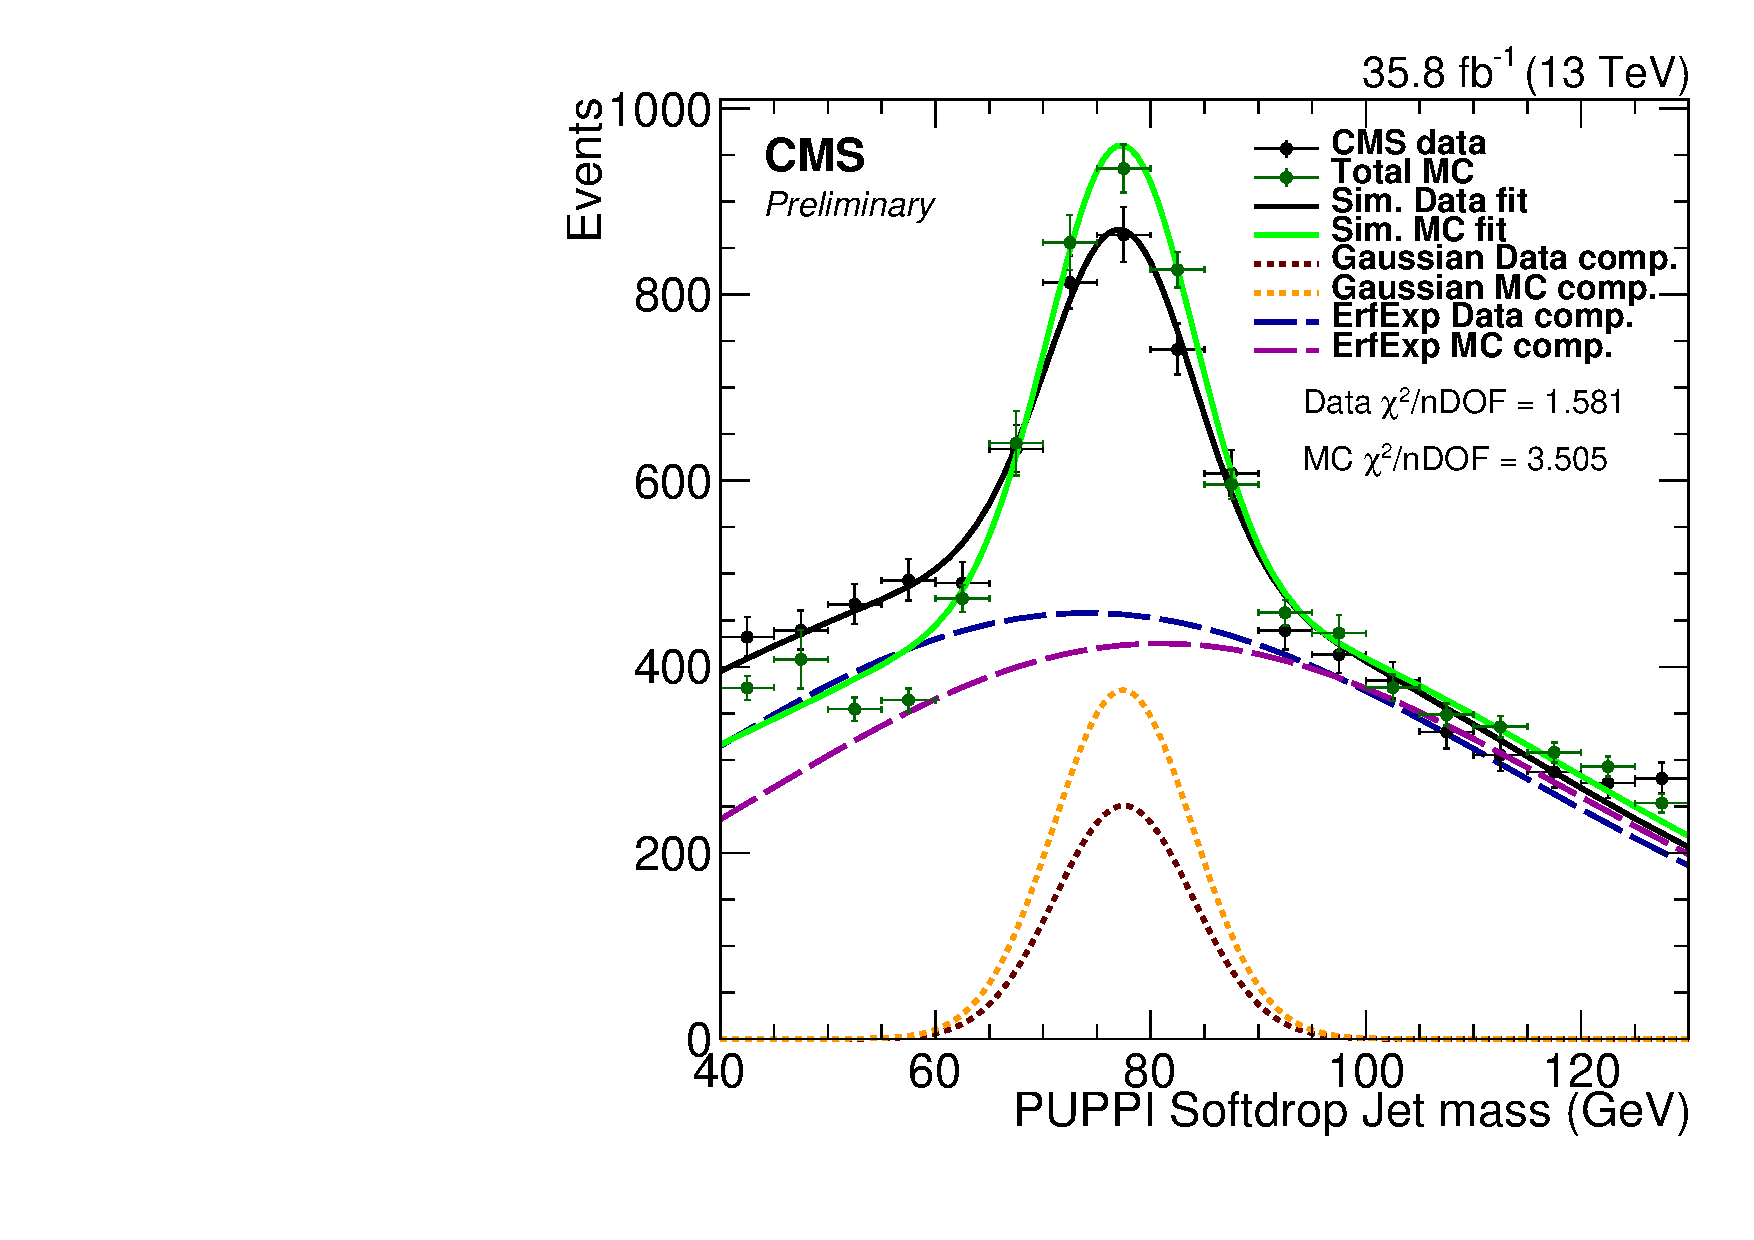
\includegraphics[width=0.45\textwidth]{figures/higgstagging/n2ddt/CombinedPlot_model_data_em_CA15.pdf}
%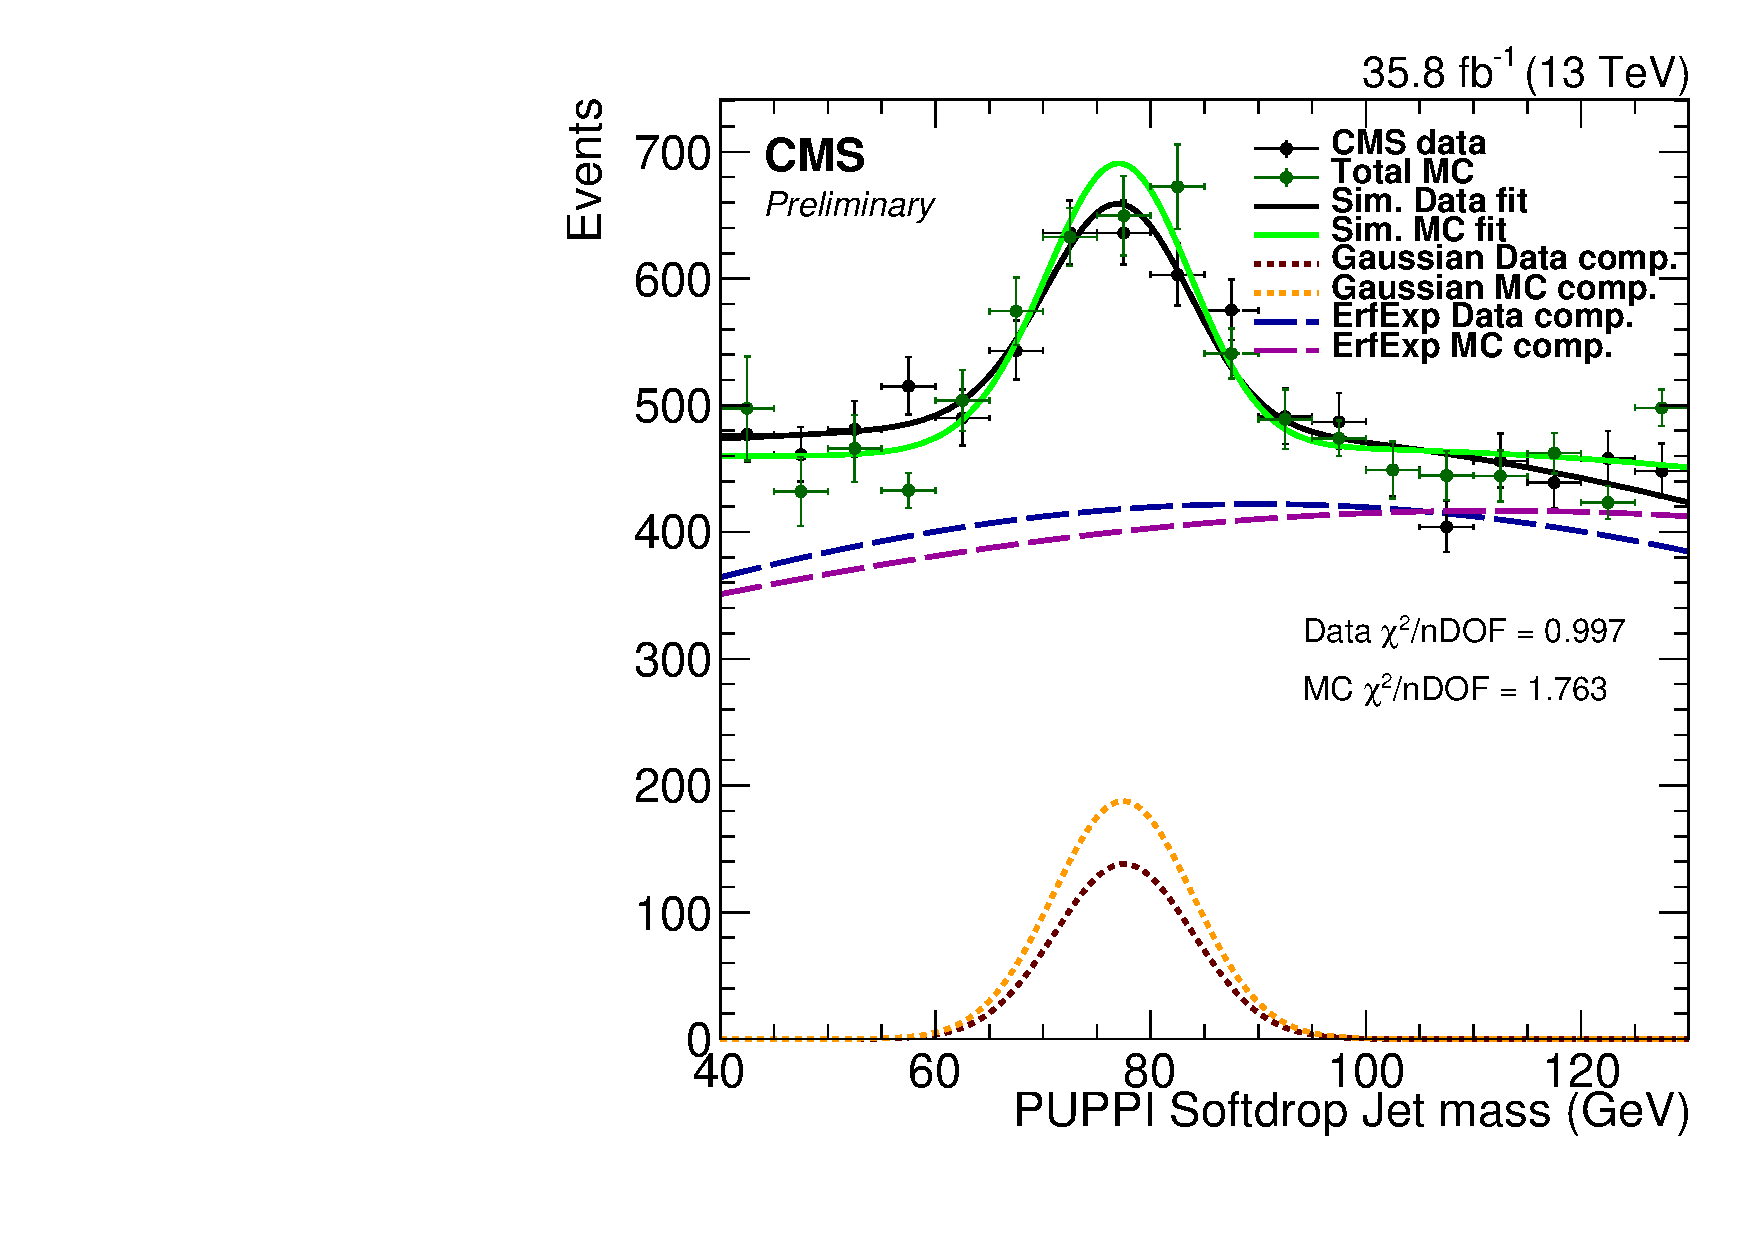
\includegraphics[width=0.45\textwidth]{figures/higgstagging/n2ddt/CombinedPlot_model_data_failN2DDTcut_em_CA15.pdf}
%\caption{Puppi softdrop mass distributions that pass(left) and fail(right) the $N_{2}^{DDT}<0$. Results are shown for both data and simulation.}
%\label{fig:TotalFits}
%\end{figure}



%Finally, Fig.~\ref{fig:n2data_1} demonstrates a very good description of the N2DDT variable in top quark jets or QCD jets dominated regions (our control regions are introduced in Section~\ref{sec:cr}). The scale factor in \ref{tab:ScaleFactors} is applied to the signal and the MC-driven backgrounds which have a massive resonances decaying into two prongs (VH, diboson). 



%\begin{figure}
%\centering
% \subfloat{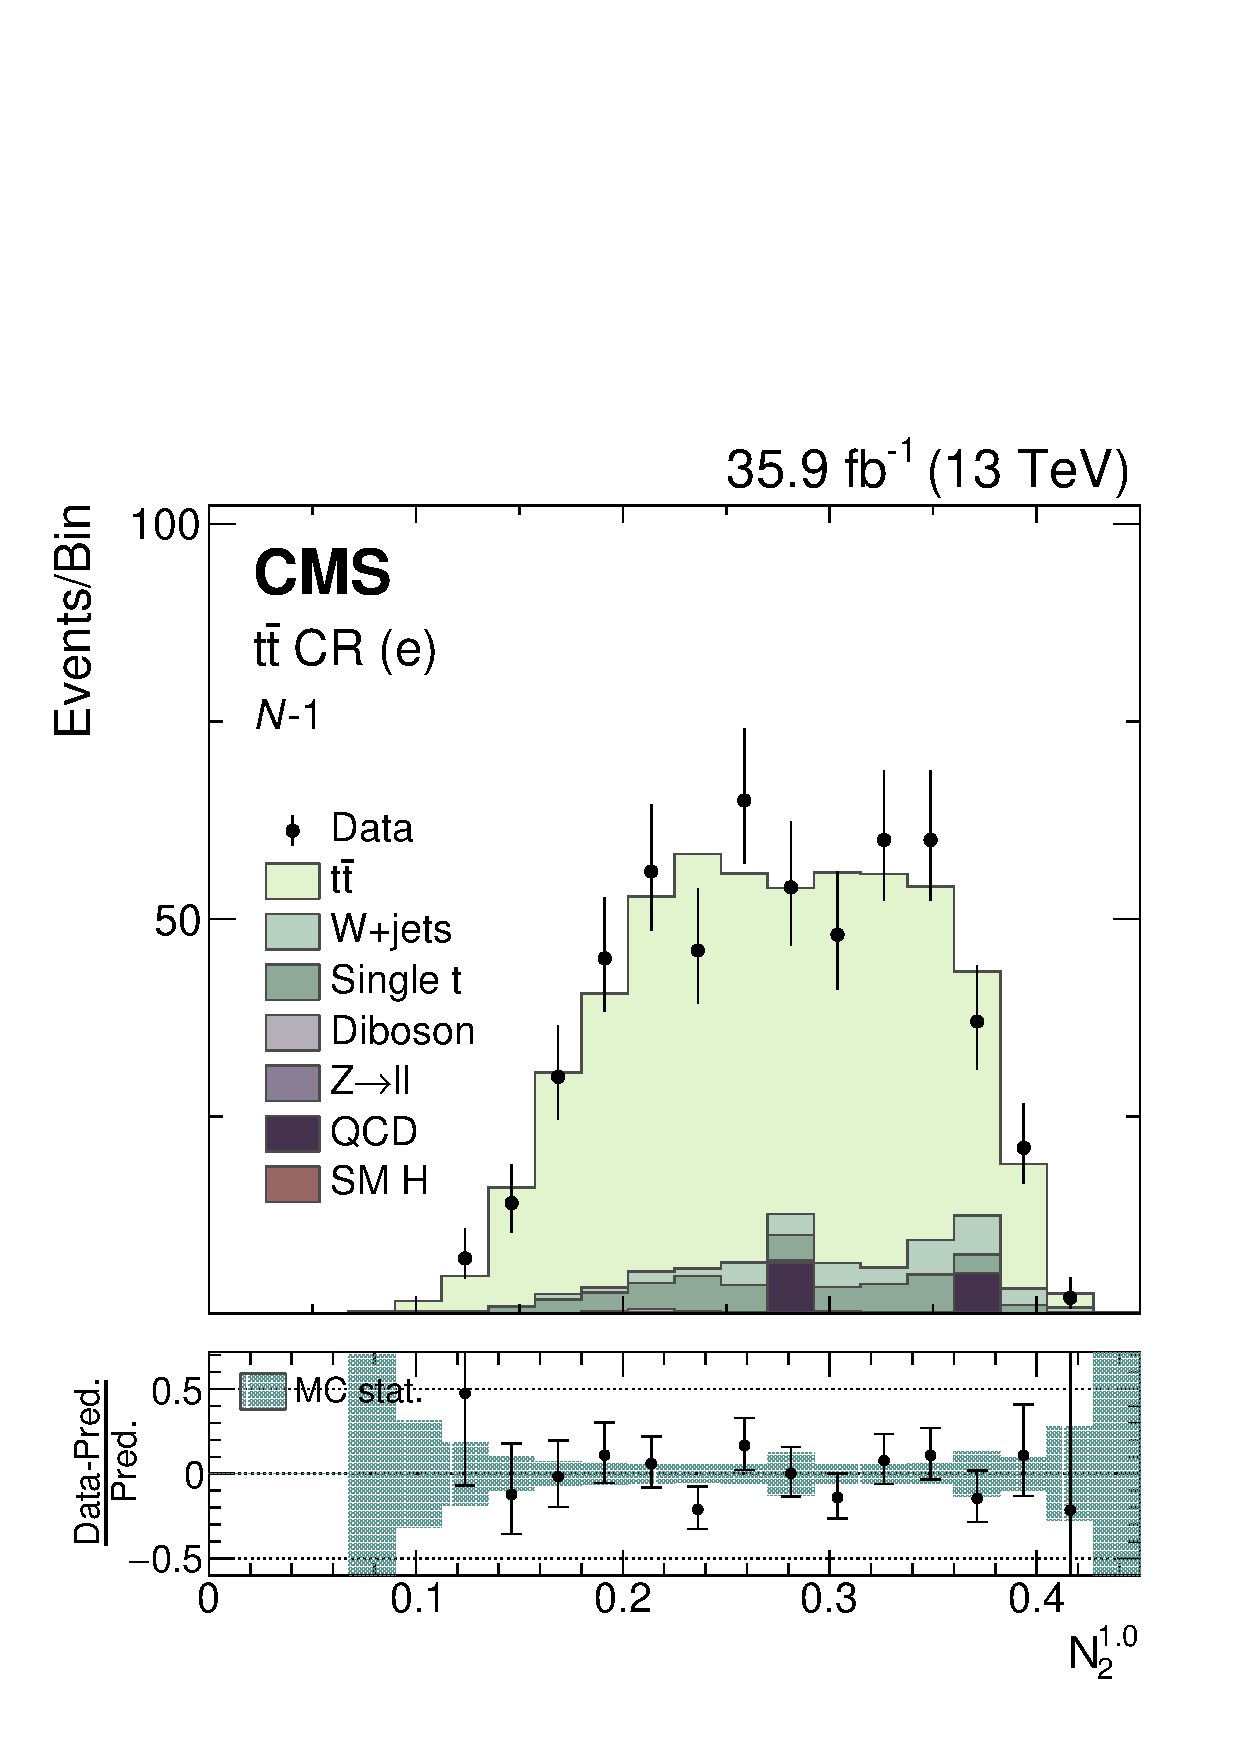
\includegraphics[width=0.33\textwidth]{figures/dataMC/cr_ttbar_el_N2_10_NM1_lumi0.pdf}}
% \subfloat{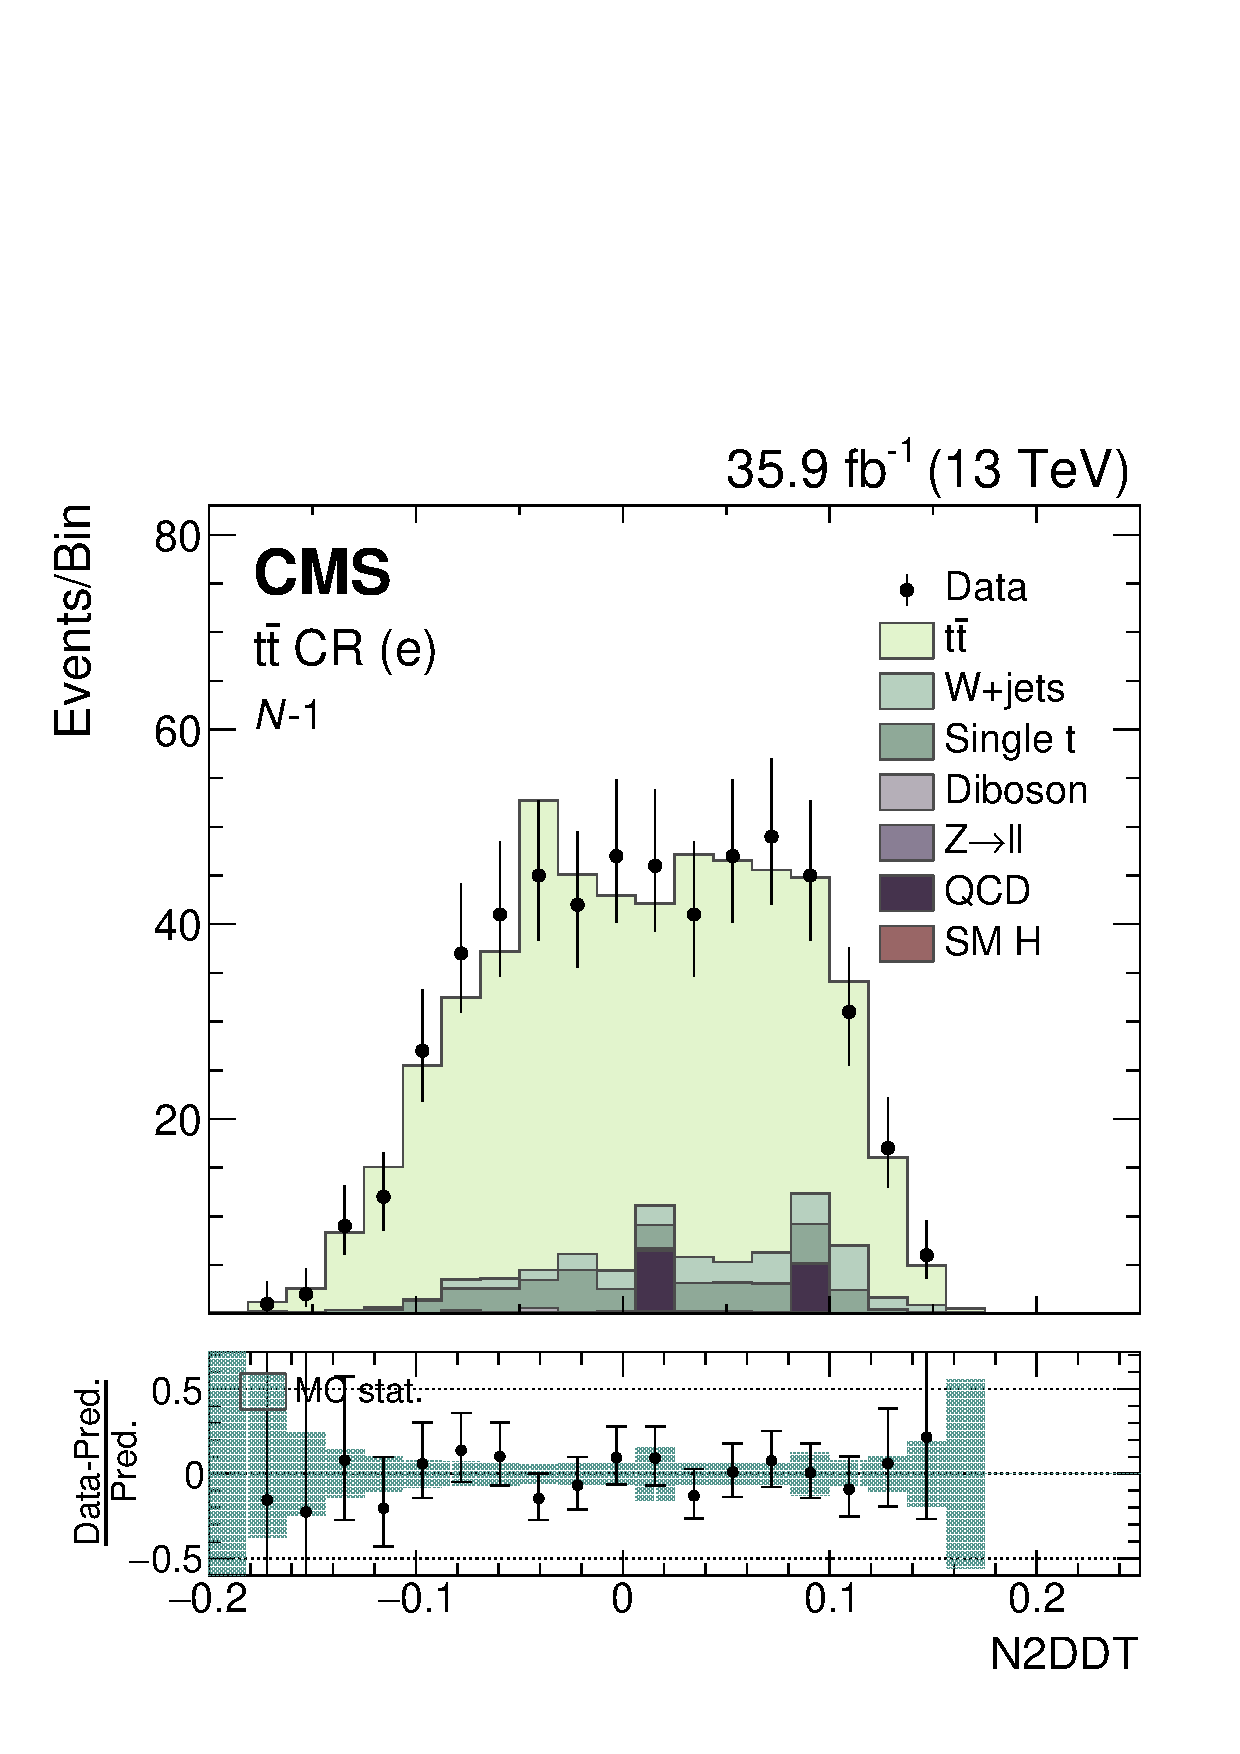
\includegraphics[width=0.33\textwidth]{figures/dataMC/cr_ttbar_el_N2DDT_NM1_lumi0.pdf}}\\
% \subfloat{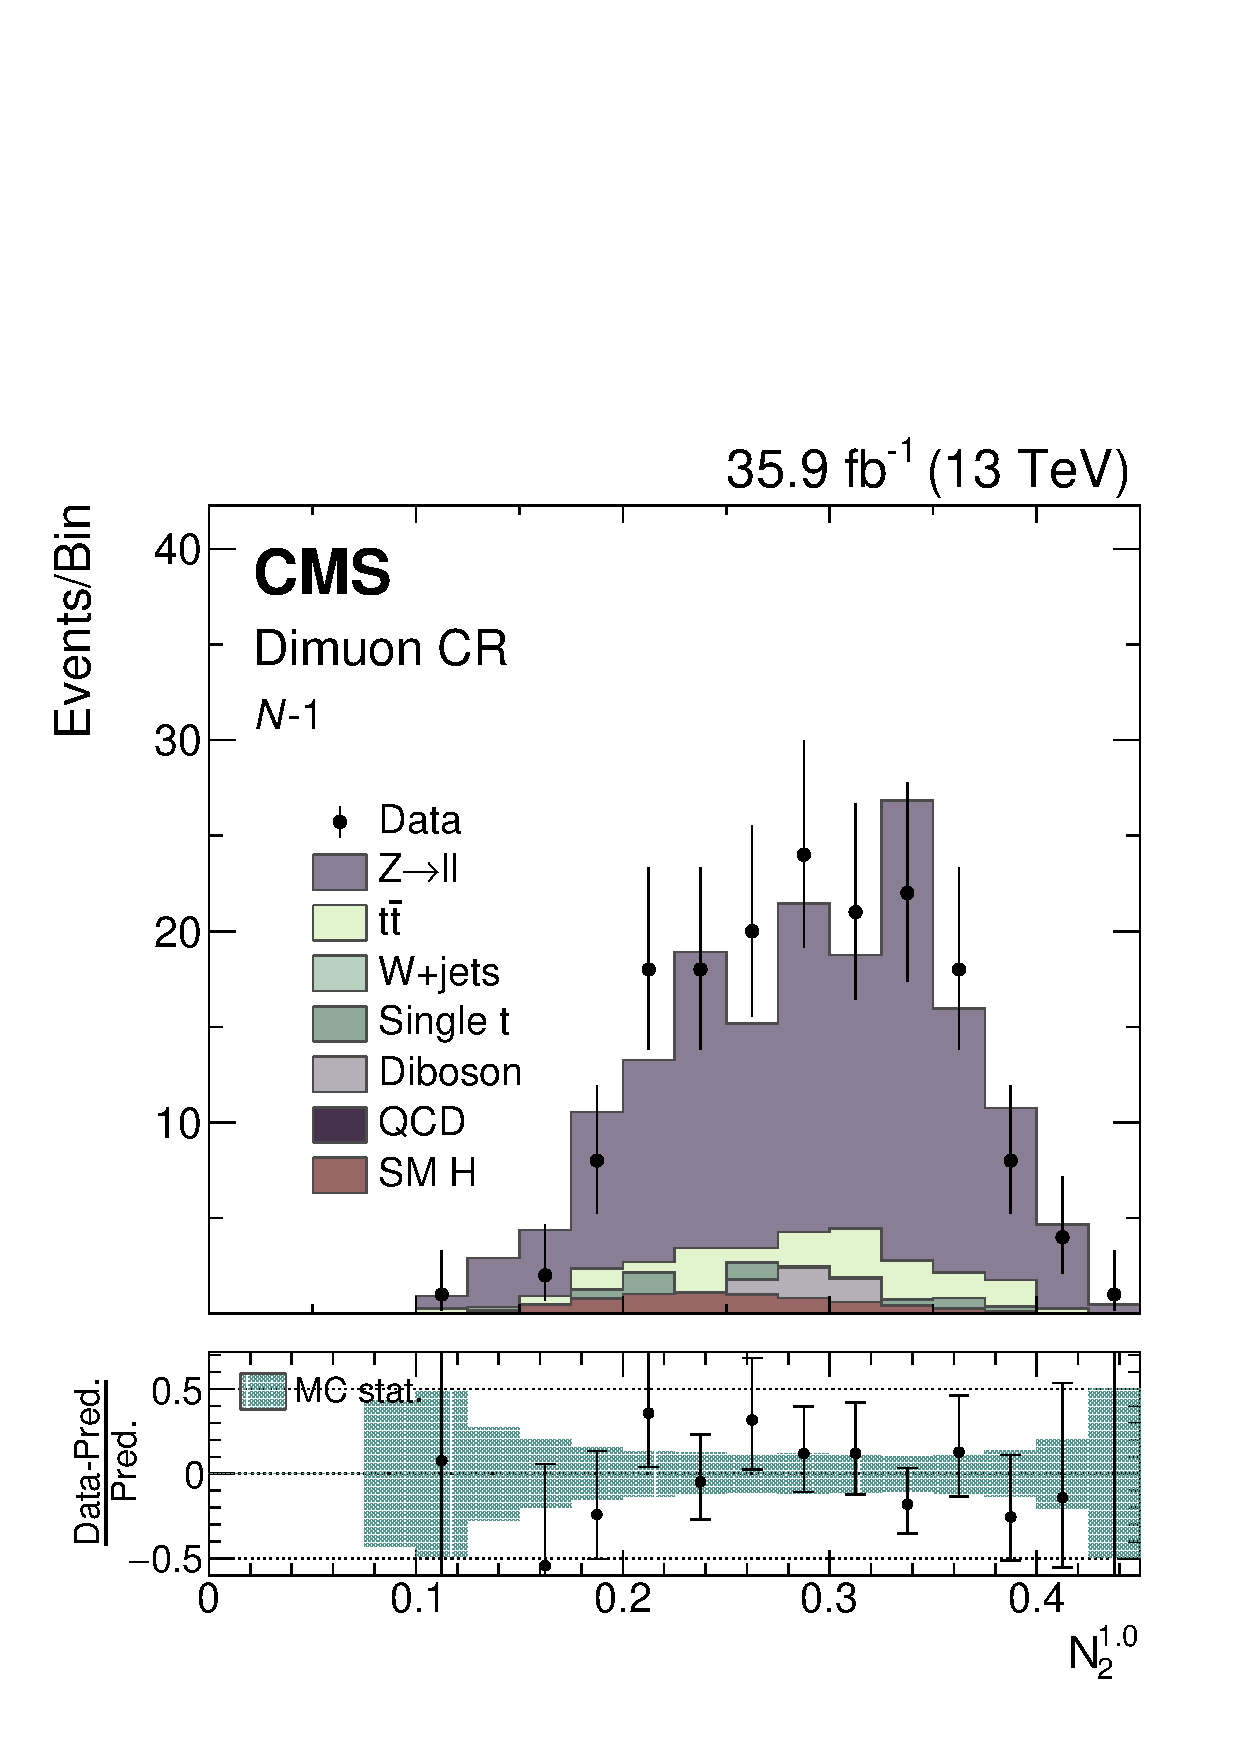
\includegraphics[width=0.33\textwidth]{figures/dataMC/cr_dimuon_N2_10_NM1_lumi0.pdf}}
% \subfloat{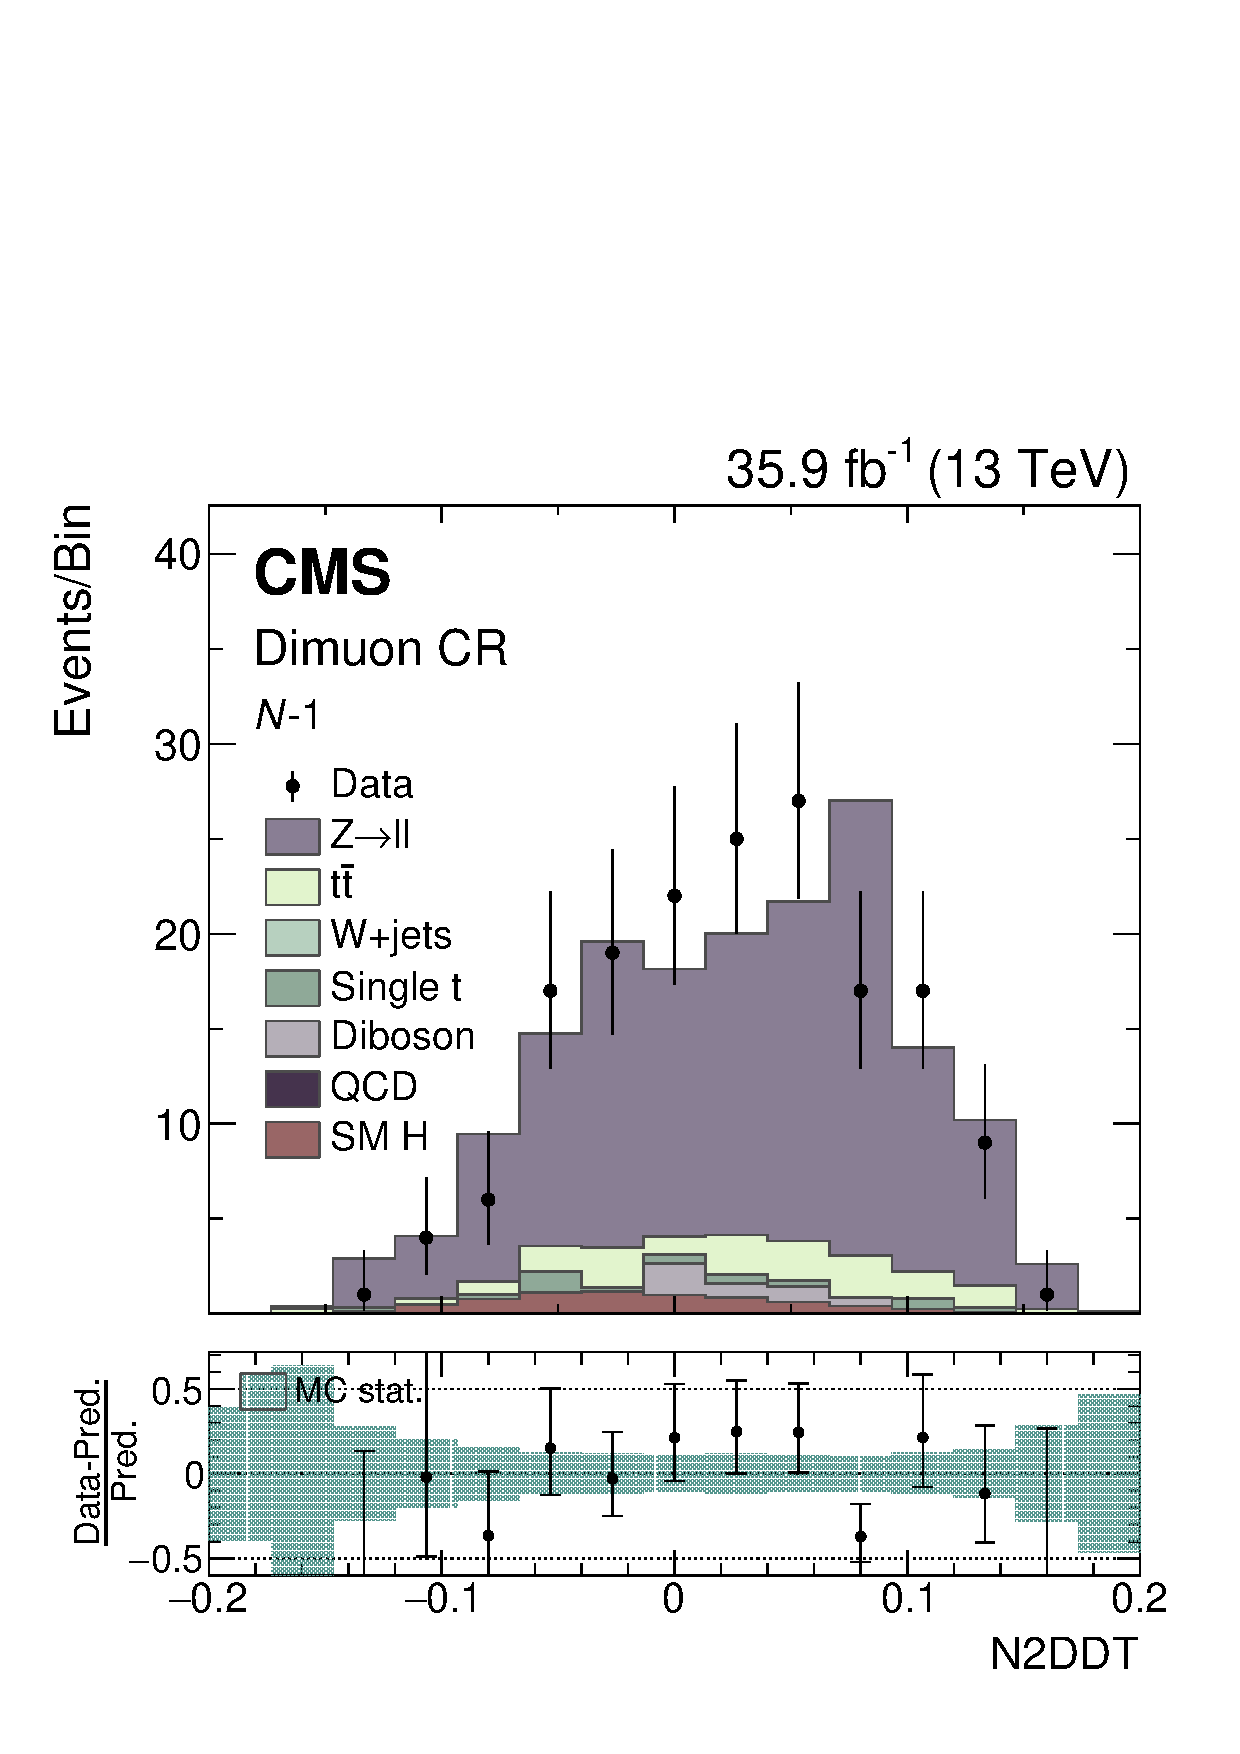
\includegraphics[width=0.33\textwidth]{figures/dataMC/cr_dimuon_N2DDT_NM1_lumi0.pdf}}\\
%\caption{Validation plots for $N_2$ and $N_2^{\text{DDT}}$  in the ttbar and dilepton control regions. No cut on N2DDT is applied. MC is normalized to data in order to facilitate the shape comparison. Very good agreement is observed. }
%\label{fig:n2data_1}
%\end{figure}




\subsection{Double-b tagger}

In this analysis we employ the double-b tagger algorithm. A general description of the tagger, which tries to identify a two-prong structure made of b quarks, is provided in~\cite{CMS-PAS-BTV-15-002}. Particularly for the CA15 case, the training of the tagger has been repeated incorporating the minimum of the CSV scores of the two leading subjets as input variables. Due to the larger cone with $R=1.5$, the clustering algorithm is able to retain a higher signal efficiency also in regimes with intermediate boost, where it is possible to clearly resolve two subjets, hence additional information can be gained from the CSV scores. This is visible from the ROC curve in Fig.~\ref{fig:doublebroc}, showing the performace of the CA15 double-b tagger version compared to tradition methods like the use of subjet CSV scores only.


\begin{figure}
  \centering
  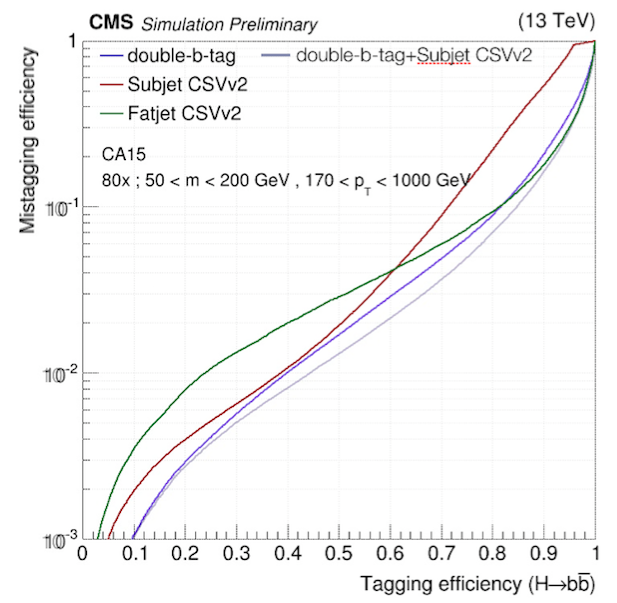
\includegraphics[width=0.475\textwidth]{figures/higgstagging/doubleb/doubleb_roc_split.png}\\
  \caption{ROC curve comparing the performance in tagging $\text{H}\to\text{b}\bar{\text{b}}$ fat jets of using either subjet CSV algorithm or double b tagger with or without the subjet CSV scores as input variables.}
  \label{fig:doublebroc}
\end{figure}

The chosen working point of double-b $> 0.75$ corresponds to the same background efficiency of the medium working point of the minimum of the CSV scores of the two leading subjets used in the previous iteration of Mono-H  analysis~\cite{CMS_AN_2016-219}, benefiting from the enhanced signal efficiency.
In terms of tagging and mistagging efficiency measurements, the analysis is precisely following what has been done in~\cite{CMS-PAS-BTV-15-002} with AK8 jets for deriving scale factors for the double-b tagger to be applied throughout the analysis. The current measurement at 13\TeV with AK8 jets is documented in~\cite{Ref:BTAG2016}. A dedicated tagging and mistagging efficiency mesurements on CA15 jet was derived~\cite{CMS_AN_2016-219} and will be applied throughout the analysis.

%\subsubsection{Tagging efficiency measurement}
%\label{tagging_efficiency}
%The Lifetime Tagging (LT) method uses the Jet Probability (JP) discriminant to measure the double-b tagging efficiency by fitting MC templates for b, c and light flavour jets to data~\cite{Ref:LT}. This discriminant uses information on the probability of tracks in a jet with positive impact parameter significance to originate from the primary interaction vertex. This parameter is calibrated in inclusive QCD multijet events using templates with negative impact parameter tracks~\cite{Ref:JP}. The calibration is performed independently in data and MC. The JP discriminant provides a good shape separation between heavy and light flavour jets over the broad jet \pt range and can be used as a fit variable to extract the fraction of heavy flavour jets in data sample.

%In the absence of a control region clean enough in Hbb events, the measurement is performed in double-muon tagged multijet events, which are enriched in gbb events serving as a good proxy for Hbb decays, as was reasoned in~\cite{CMS-PAS-BTV-15-002}. The simulated datasets used are listed in Tab.~\ref{Tab:QCDMultijet}. Muon−enriched samples obtained by requiring a muon with $\pt> 5\GeV$ at the generator level are used in association with BTagMu data corresponding to the full integrated luminosity available from the year 2016. Triggers as listed in Tab.~\ref{Tab:Triggers} are employed.




%\begin{table}[htb]
% \begin{center}
%\footnotesize
%  \caption{QCD MC samples used in the efficiency measurement.}
%\begin{tabular}{lr}
%\hline\hline
%{\bf Muon-enriched MC} & \\
%\vspace{2mm} Sample & $\sigma $ [pb]  \\
%\hline
%QCD\_Pt\_170to300\_MuEnrichedPt5\_TuneCUETP8M1\_13TeV\_pythia8 & $8.65 \cdot 10^3$ \\
%QCD\_Pt\_300to470\_MuEnrichedPt5\_TuneCUETP8M1\_13TeV\_pythia8 & $7.97 \cdot 10^2$ \\
%QCD\_Pt\_470to600\_MuEnrichedPt5\_TuneCUETP8M1\_13TeV\_pythia8 & $7.90 \cdot 10^1$ \\
%QCD\_Pt\_600to800\_MuEnrichedPt5\_TuneCUETP8M1\_13TeV\_pythia8 & $2.51 \cdot 10^1$ \\
%QCD\_Pt\_800to1000\_MuEnrichedPt5\_TuneCUETP8M1\_13TeV\_pythia8 & $4.71$ \\
%QCD\_Pt\_1000toInf\_MuEnrichedPt5\_TuneCUETP8M1\_13TeV\_pythia8 & $1.62$ \\
%\hline
%\end{tabular}
%\normalsize
%  \label{Tab:QCDMultijet}
%\end{center}
%\end{table}

%CA15 jets with $|\eta| < 2.4$ were selected, with the jets passing the ``tight'' jet ID requirement~\cite{JetID13TeVTWiki}. The soft drop algorithm was used to resolve the CA15 jets into substructures, henceforth called soft drop subjets. Muon-tagging of jets is used to enrich them in $B$ hadrons. Both the subjet and the double-b tagger performance measurements use AK8 jets containing muon-tagged subjets, with the following muon ID requirement:

%\begin{itemize}
%\item Global PF muon with $\pt > 7\GeV$ and $|\eta| < 2.4$;
%\item N (hits in muon chambers) $> 0$;
%\item N(matched muon stations) $> 1$;
%\item N(hits in tracker layers) $> 7$;
%\item N(hits in pixel layers) $> 0$;
%\item N(missing outer hits) $< 99$;
%\item $\chi^{2}$/ndf from global track $< 10$;
%\item $\pt(\mu)/\pt({\rm jet})  < 0.5$;
%\item $\Delta R(\mu, {\rm subjet}) < 0.4$;
%\end{itemize}

%For the double b-tagger measurements, the CA15 jets are required to have $\pt > 200\GeV$, divided in the ``low \pt'' ($200 < \pt < 350\GeV$) and the ``high \pt'' ($\pt > 350\GeV$) ranges. We use the official pile-up reweighting, as well as MC JP calibration on both data and MC.
%We reweight the MC $\pt$ distribution to match the data distribution in order to account for triggers being absent from certain data runs. Lastly, we remove any jet from a QCD sample with $p_{T}$ $<$ 300 GeV that has high weight or that comes from an event with high jet multiplicity, in order to prevent large spikes in the JP distribution used to calculate the scale factor.

%The final selection features:

%\begin{itemize}
%\item Muon $p_\text{T}\text{'s}>7$\,GeV
%\item $\text{pruned~jet~mass}>50$\,GeV
%\item $p_\text{T}(\mu_1+\mu_2)<0.6\,p_\text{T}(\text{jet})$ in order to guarantee for sufficient hadronic activity in the jet 
%\end{itemize}


%\begin{table}[htbp]
%  \begin{center}
%    \topcaption{Trigger requirements for double b-tagging in different \pt bins.}\label{tab:BoostedTrigs}
%    \begin{tabular}{c|c} 
%      \hline\hline
%      Range in fat jet \pt & Trigger\\ 
%      \hline 
%      $>350$ &    \texttt{BTagMu\_AK8Jet300\_Mu5} \\
%      200-350 & \texttt{BTagMu\_DiJet170\_Mu5} \\
%      \hline\hline
%    \end{tabular}
%  \label{Tab:Triggers}
%  \end{center}
%\end{table}


%Commissioning plots of some of the input variables are presented in Fig.~\ref{fig:doublebdata_1}. The final double-b tagger discriminant is shown in the same Figure, as is the JP distribution that is used for extracting the scale factor in the fit explained in the following. Shapes for the different components for both \pt bins are shown in Fig.~\ref{fig:double_shapes} for the pretag and pass regions. The properly normalized postfit templates are shown in \ref{fig:double_shapes_norm}.

%\begin{figure}
%\centering
% \subfloat{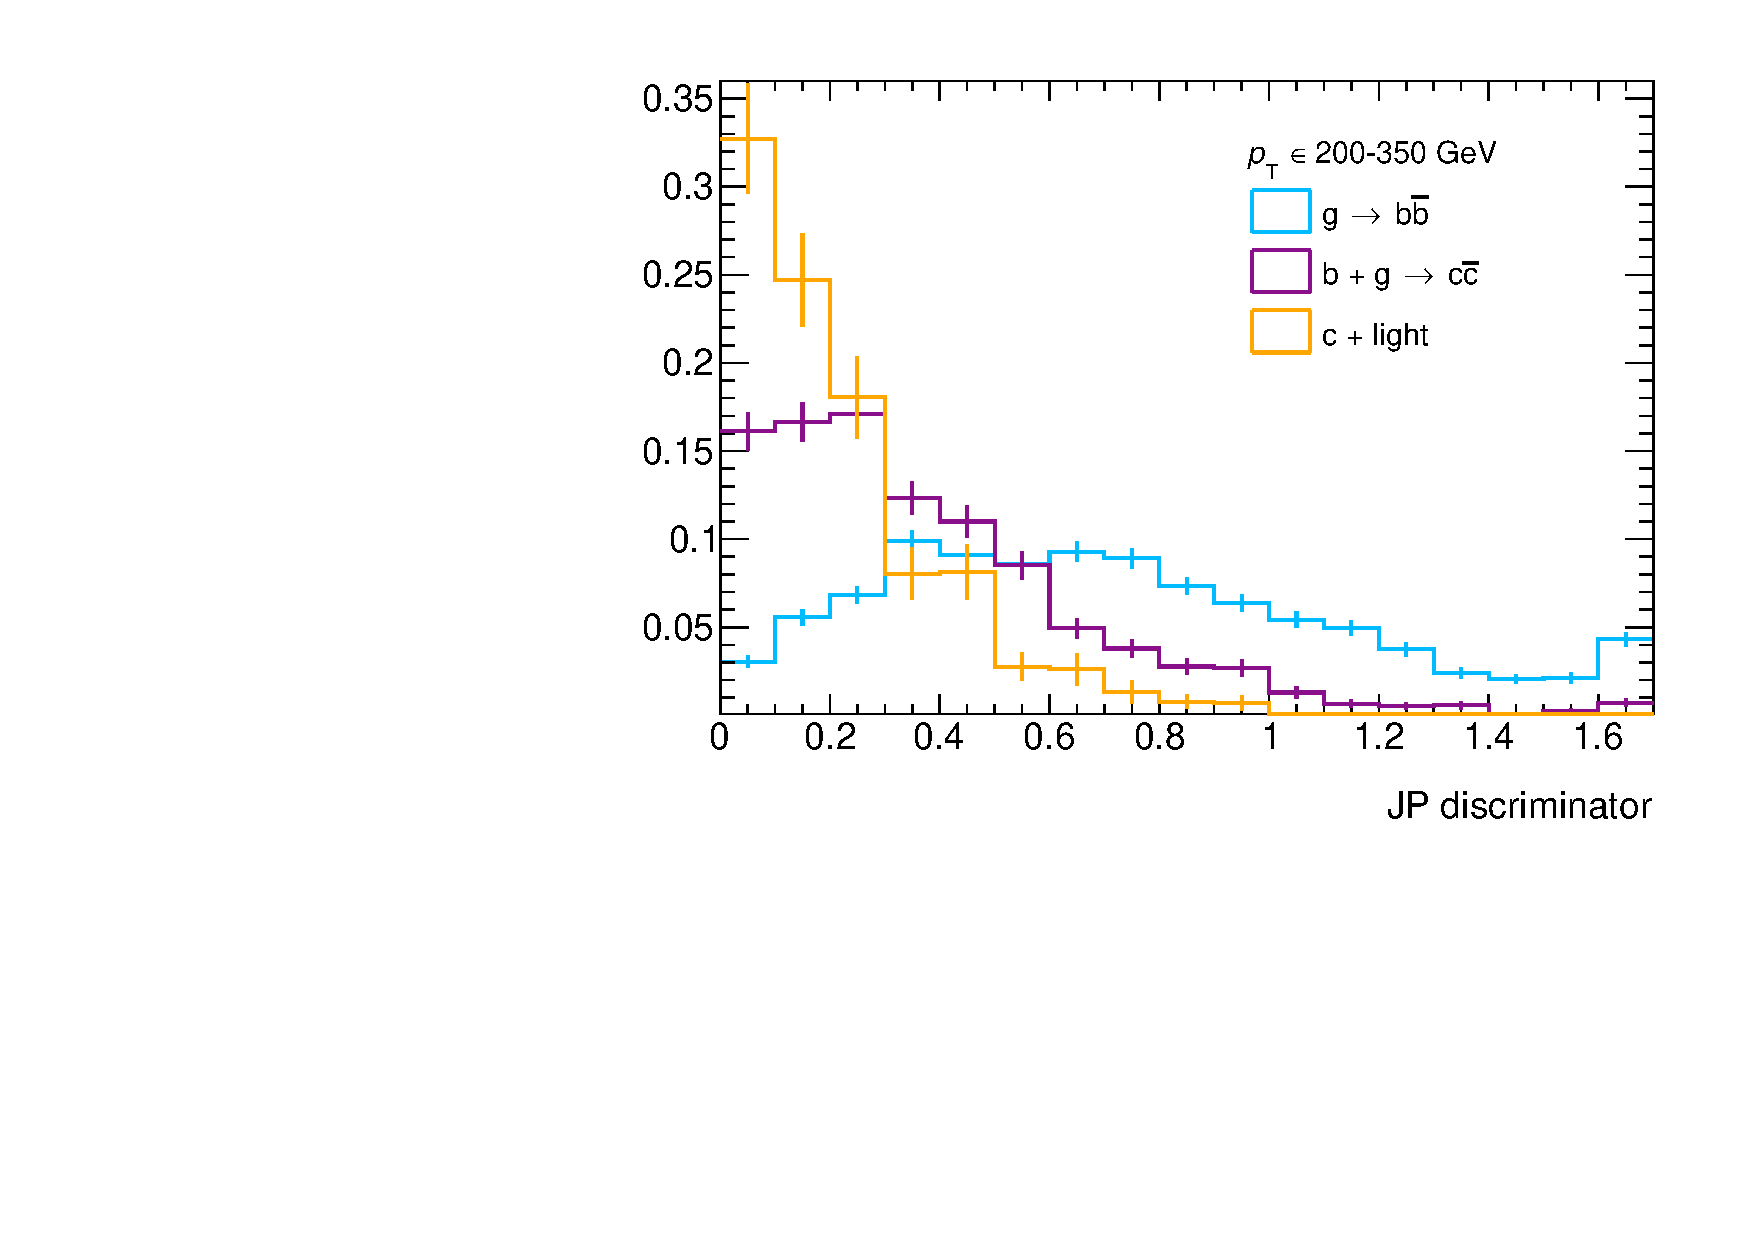
\includegraphics[width=0.45\textwidth]{figures/higgstagging/doubleb/doubleBM2ptlow/pics/shape.pdf}}
% \subfloat{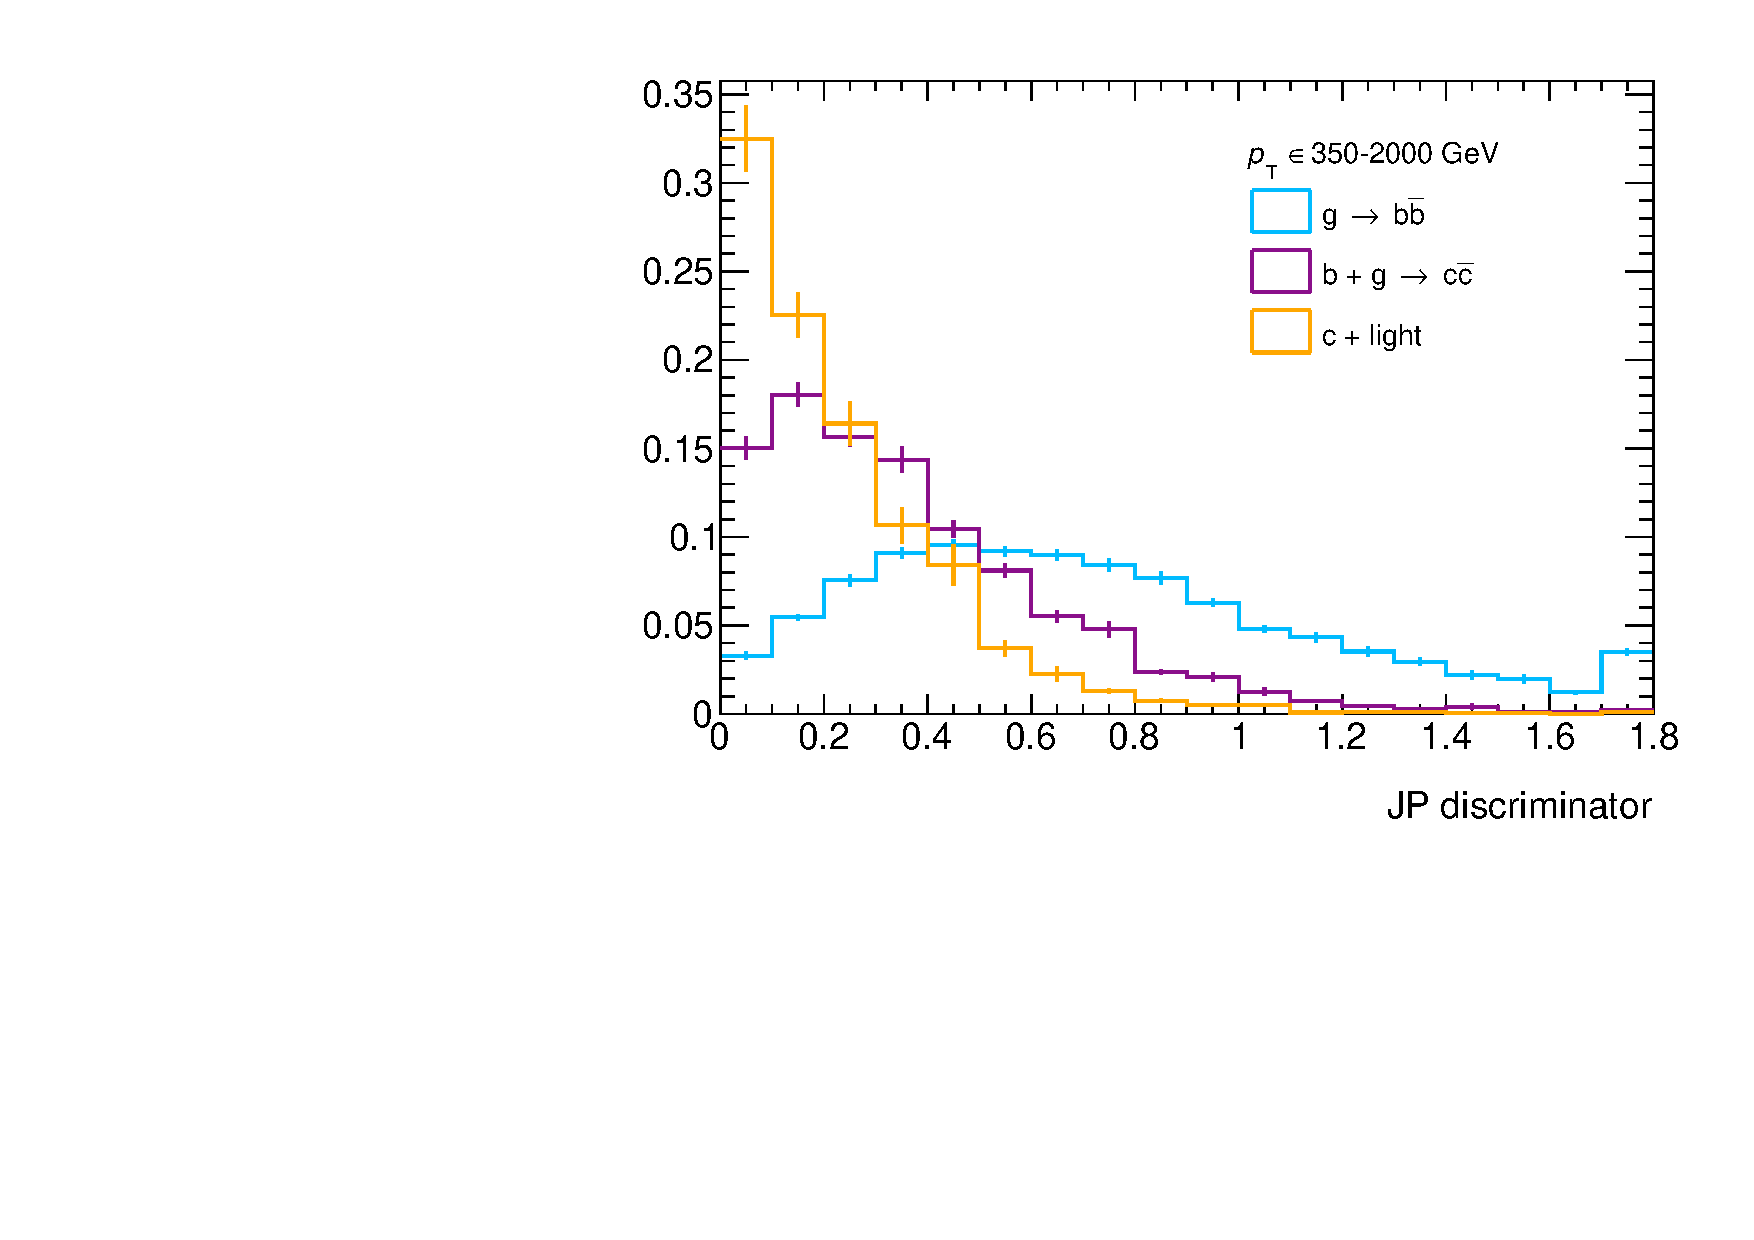
\includegraphics[width=0.45\textwidth]{figures/higgstagging/doubleb/doubleBM2pthigh/pics/shape.pdf}}\\
% \subfloat{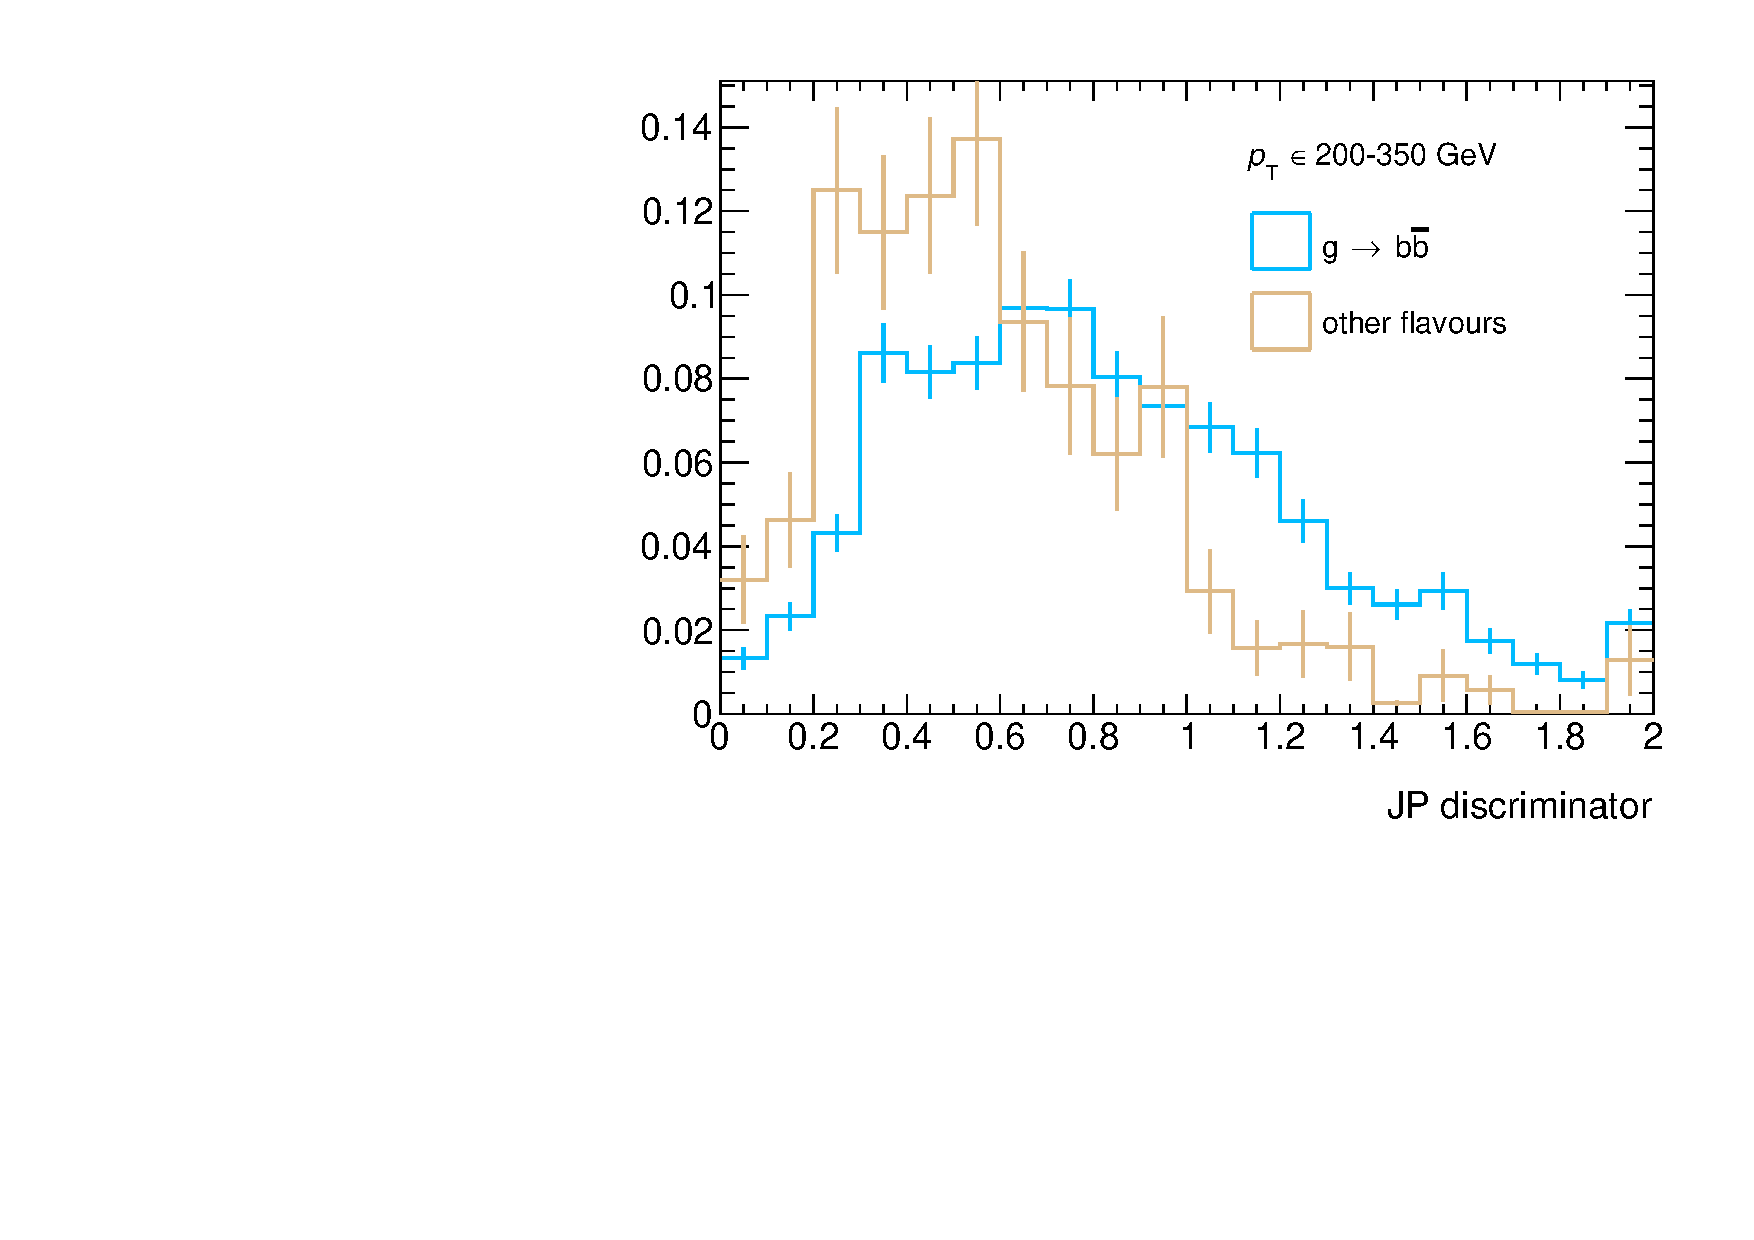
\includegraphics[width=0.45\textwidth]{figures/higgstagging/doubleb/doubleBM2ptlow/pics/shape_tag.pdf}}
% \subfloat{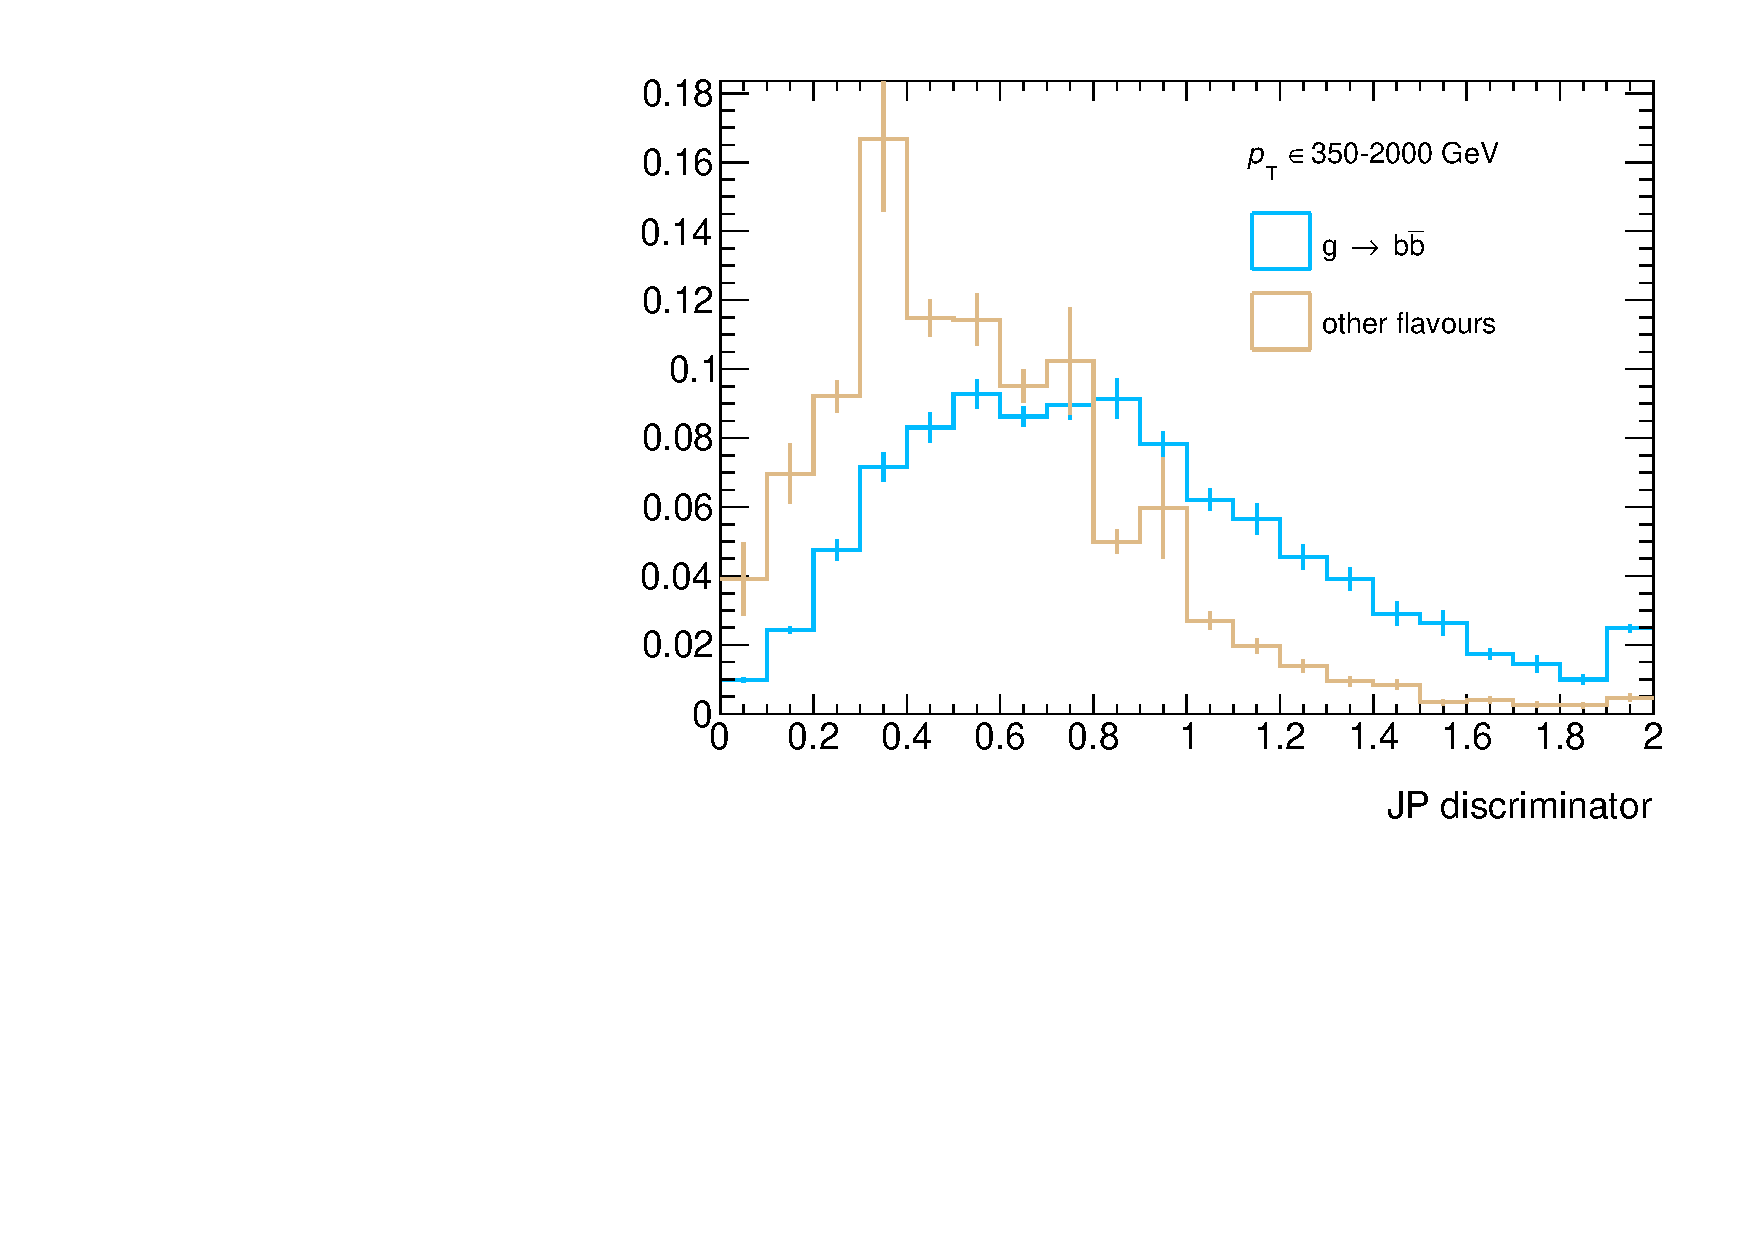
\includegraphics[width=0.45\textwidth]{figures/higgstagging/doubleb/doubleBM2pthigh/pics/shape_tag.pdf}}\\
%\caption{Shape comparison of the jet probability in the double-muon tagged multijet samples for various flavours contained in the fat jet for the pretag region (top row) and the pass bin (bottom row), for both \pt bins.}
%\label{fig:double_shapes}
%\end{figure}

%\begin{figure}
%\centering
% \subfloat{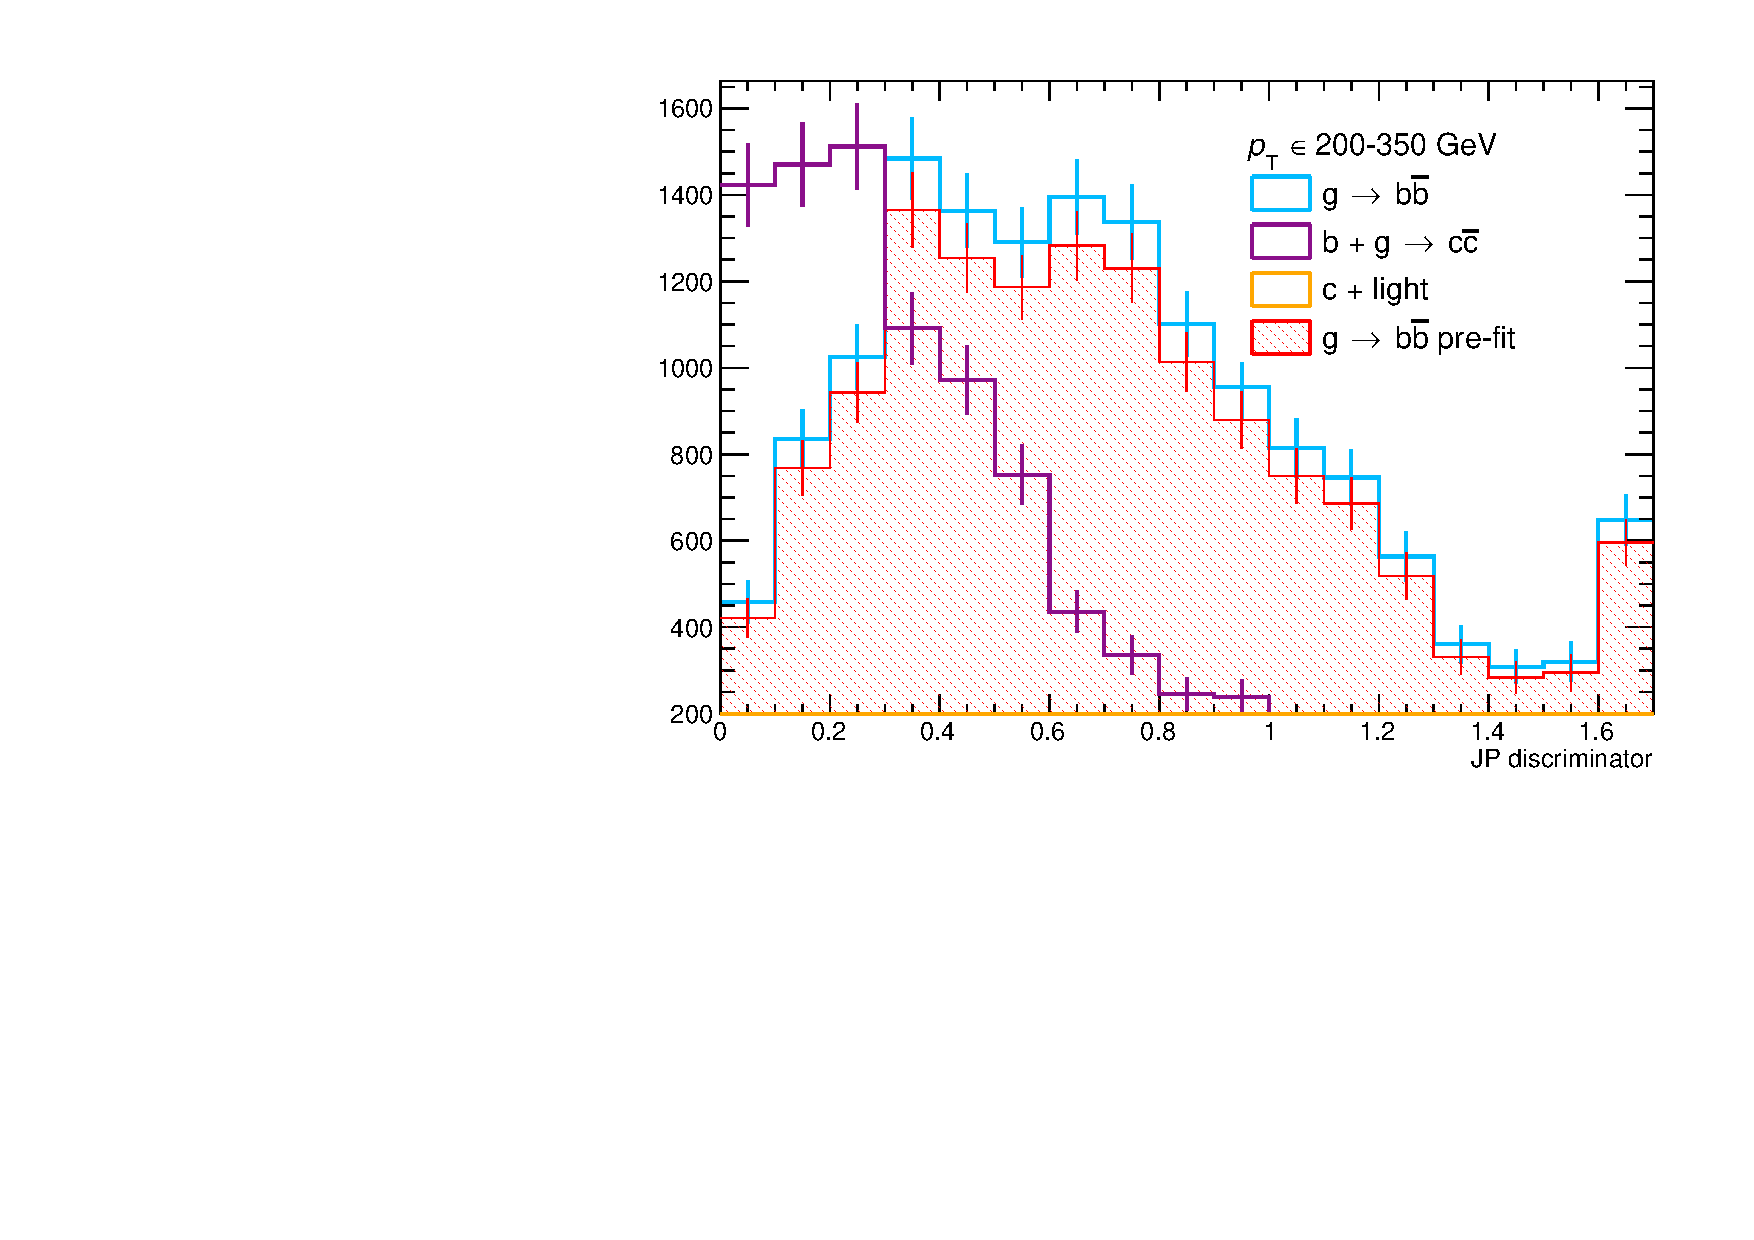
\includegraphics[width=0.45\textwidth]{figures/higgstagging/doubleb/doubleBM2ptlow/pics/shape_norm.pdf}}
% \subfloat{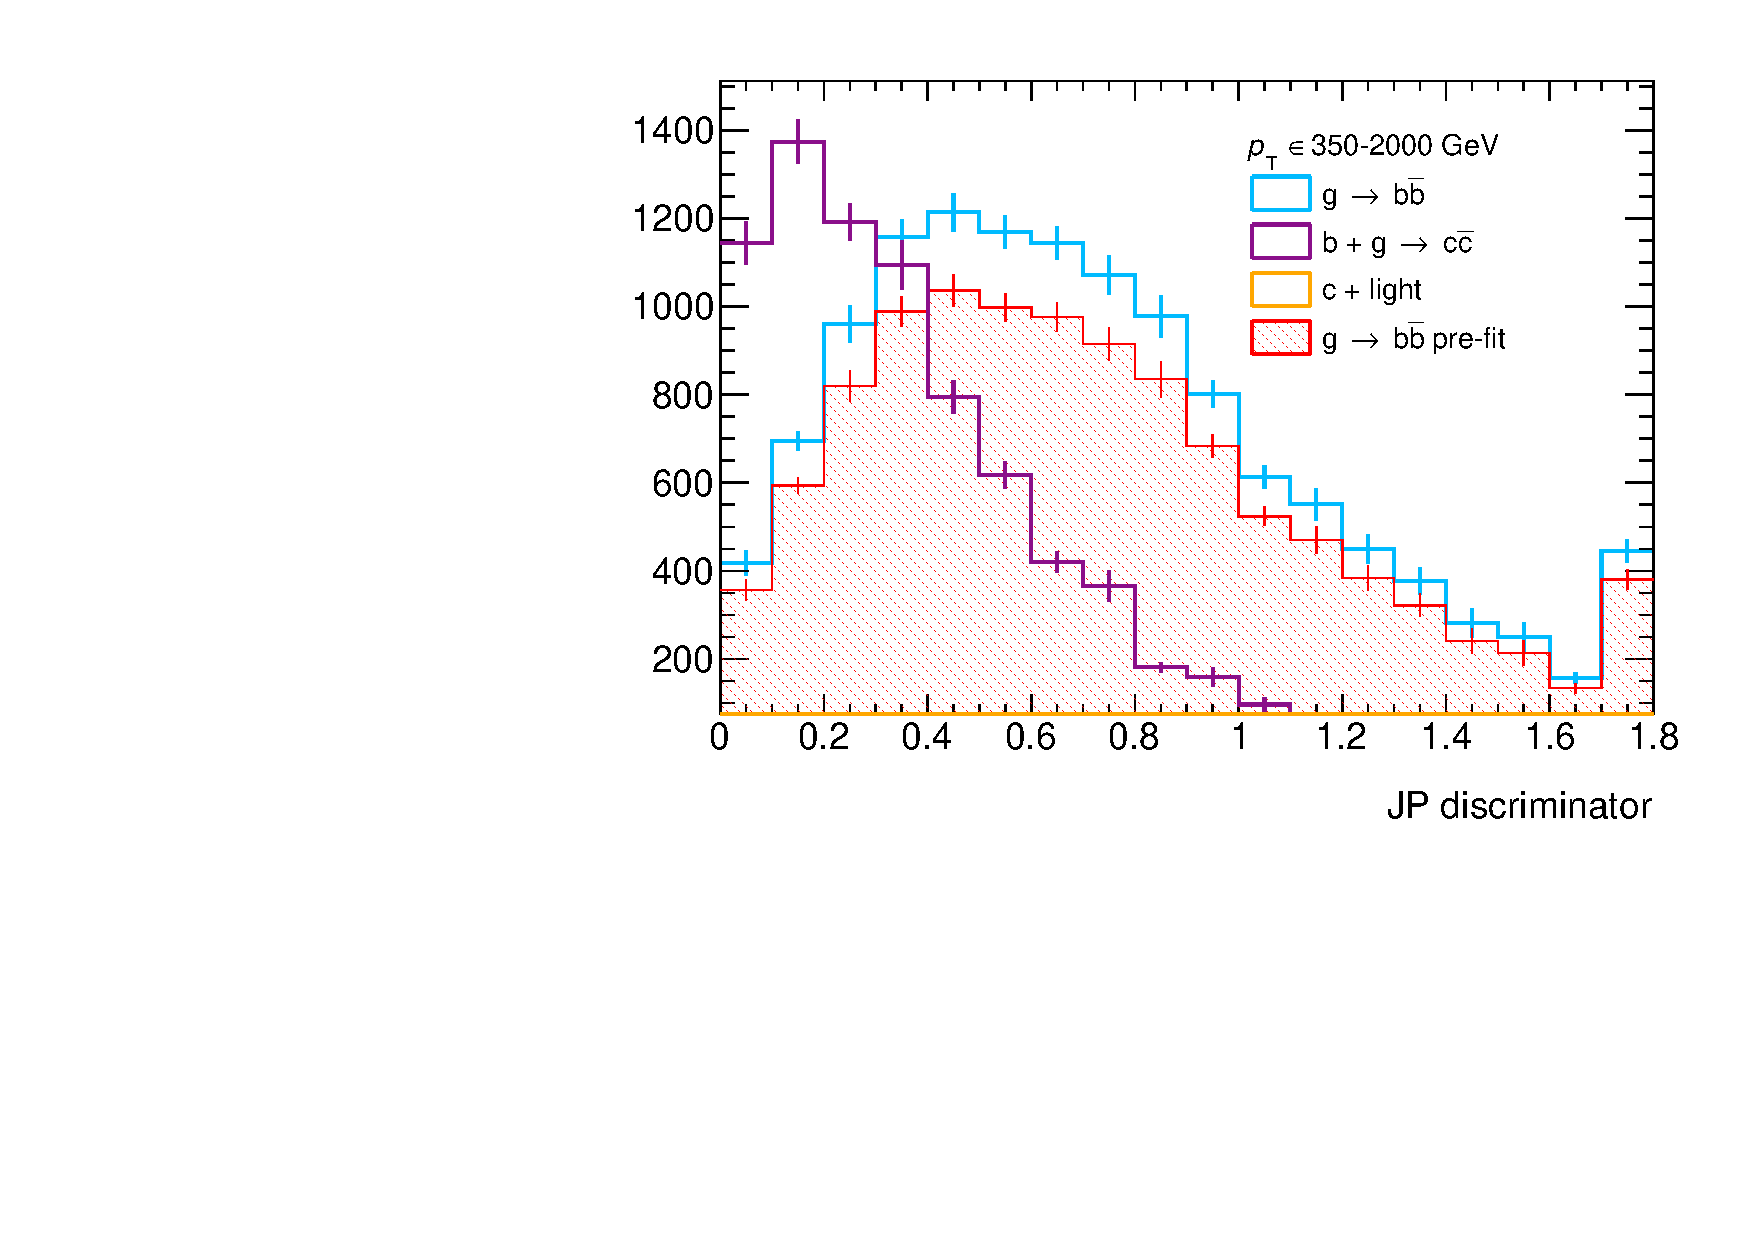
\includegraphics[width=0.45\textwidth]{figures/higgstagging/doubleb/doubleBM2pthigh/pics/shape_norm.pdf}}\\
% \subfloat{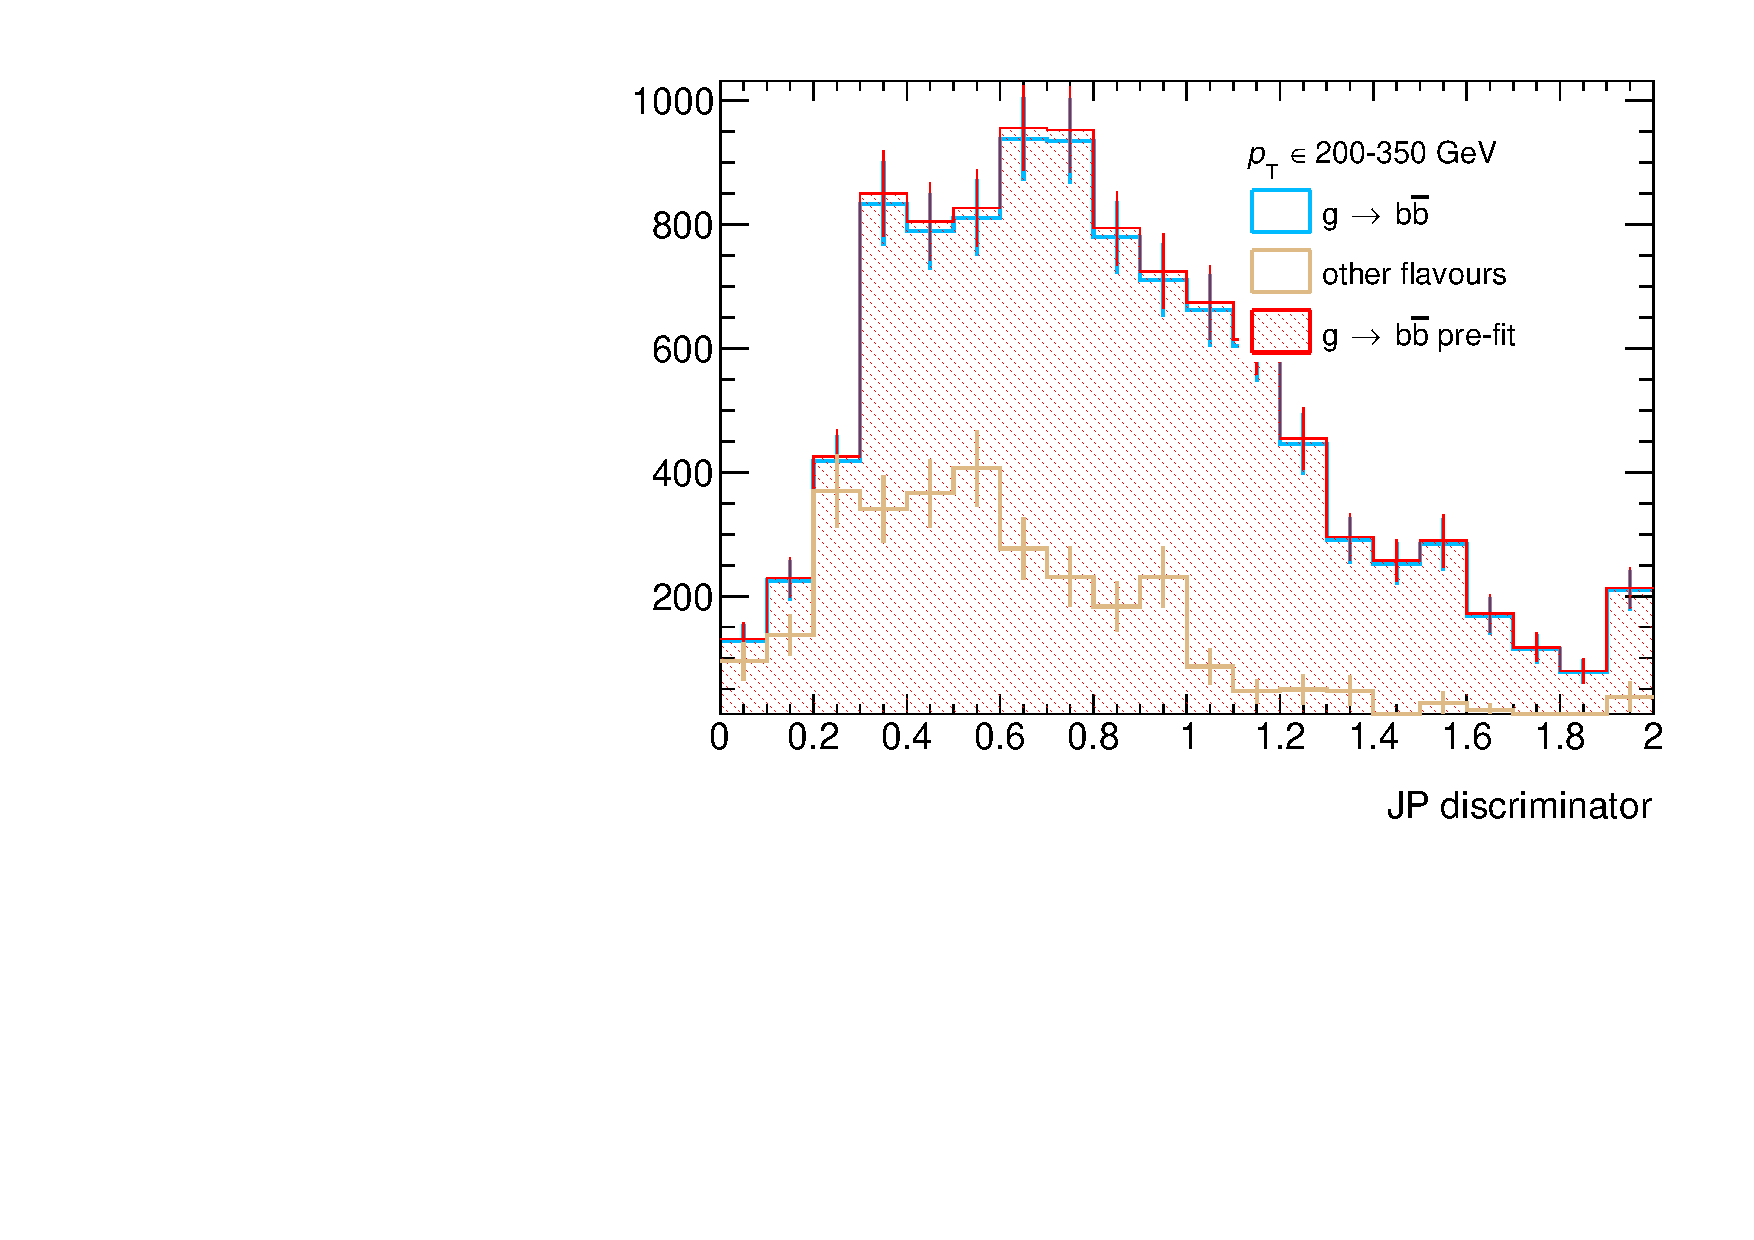
\includegraphics[width=0.45\textwidth]{figures/higgstagging/doubleb/doubleBM2ptlow/pics/shape_tag_norm.pdf}}
% \subfloat{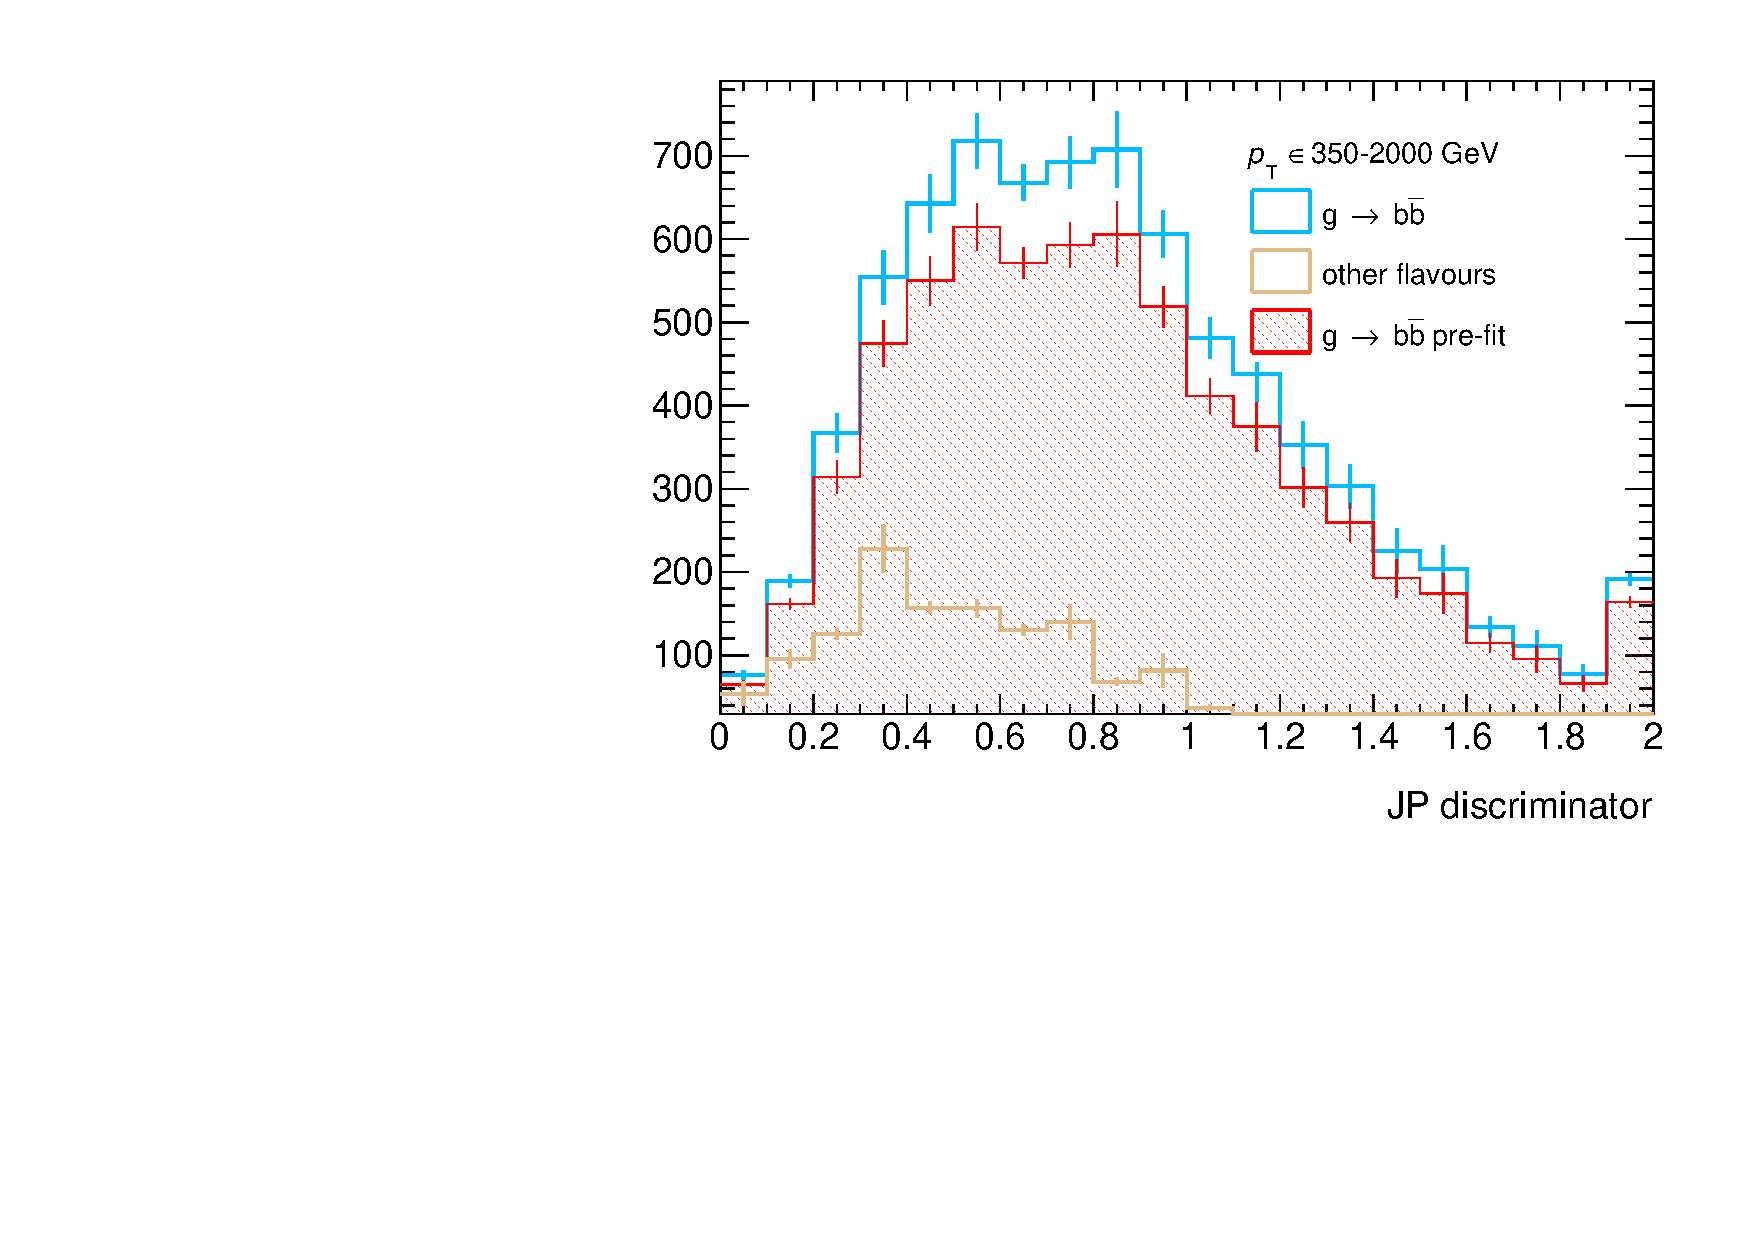
\includegraphics[width=0.45\textwidth]{figures/higgstagging/doubleb/doubleBM2pthigh/pics/shape_tag_norm.pdf}}\\
%\caption{Comparison of the jet probability in the double-muon tagged multijet samples for various flavours contained in the fat jet for the pretag region (top row) and the pass bin (bottom row), for both \pt bins, normalized to the postfit yields. For the signal template, also the prefit distribution is shown. The SF of 0.91 for the low-$p_\text{T}$~bin is reflected in the difference between the blue and red templates comparing prefit and postfit, respectively.}
%\label{fig:double_shapes_norm}
%\end{figure}


%Given the discimination power of this variable, by fitting separately in both the pretag and pass regions, the relative fractions of the various flavours can be determined, and a scale factor given by 

%\begin{equation}
%\text{SF}=\frac{\epsilon_{\text{data}}}{\epsilon_{g\to b\bar{b}~\text{MC}}},
%\end{equation}

%where data is understood to be represented by the $g\to b\bar{b}$ postfit templates.
%As several background processes are being varied as a combined template in the fit procedure, the results are sensitive to the prediction of the flavour composition of this background sample. Before applying the b tagging requirement, two background templates are considered. Contributions from single-b production and c from gluon splitting are combined together, as well as single-c and light jets. After the tagging all background processes are treated as one template. The fitted distributions for JP discriminant in the pretag region as well as in the pass bin are presented in Fig.~\ref{fig:doublebdata_2}. 

%A corresponding uncertainty on the scale factor is estimated by conservatively varying the normalization of each subcontribution of background by $\pm 50\%$. As a cross check, the scale factor derivation is also performed using all subcontributions as individual templates in the fit. Systematics related to the JP calibration are calculated by comparing the scale factor calculated using MC JP calibration on data and MC (nominal) to the scale factor calculated using data JP calibration on data and MC calibration on MC. Several sources of systematic uncertainties are accounted for. The systematics on the scale factor due to jet energy corrections, bad modelling of the number of tracks distributions, the branching ratios for c hadrons to muons, the b and fragmentation function, uncertainties on the fragmentation rate of a c quark to various D mesons, and the K$_S$ and $\Lambda$ fraction, are all found to be negiligble. The dominant systematic uncertainties are coming from varying the single-b or c from gluon content down/up by 50\% and by applying the data JP calibration (instead of the MC JP calibration) to data. These uncertainties amount to $\sim2\%$ on the scale factor. The final scale factor are provided in Table~\ref{tab:Doubleb_FitParameters1}. These scale factors are used in the maximum-likelihood fit explained in Section~\ref{sec:results} to correct the signal process and VH processes. Contributions from events with a $g\to b\bar{b}$-induced fat jet will be corrected in-situ during the fit with appropriate scale factors that apply to the soup of QCD jets accompanying W or Z bosons (i.e. in the W+jets or Z+jets background). More details are provided there.





%\begin{figure}
%\centering
% \subfloat{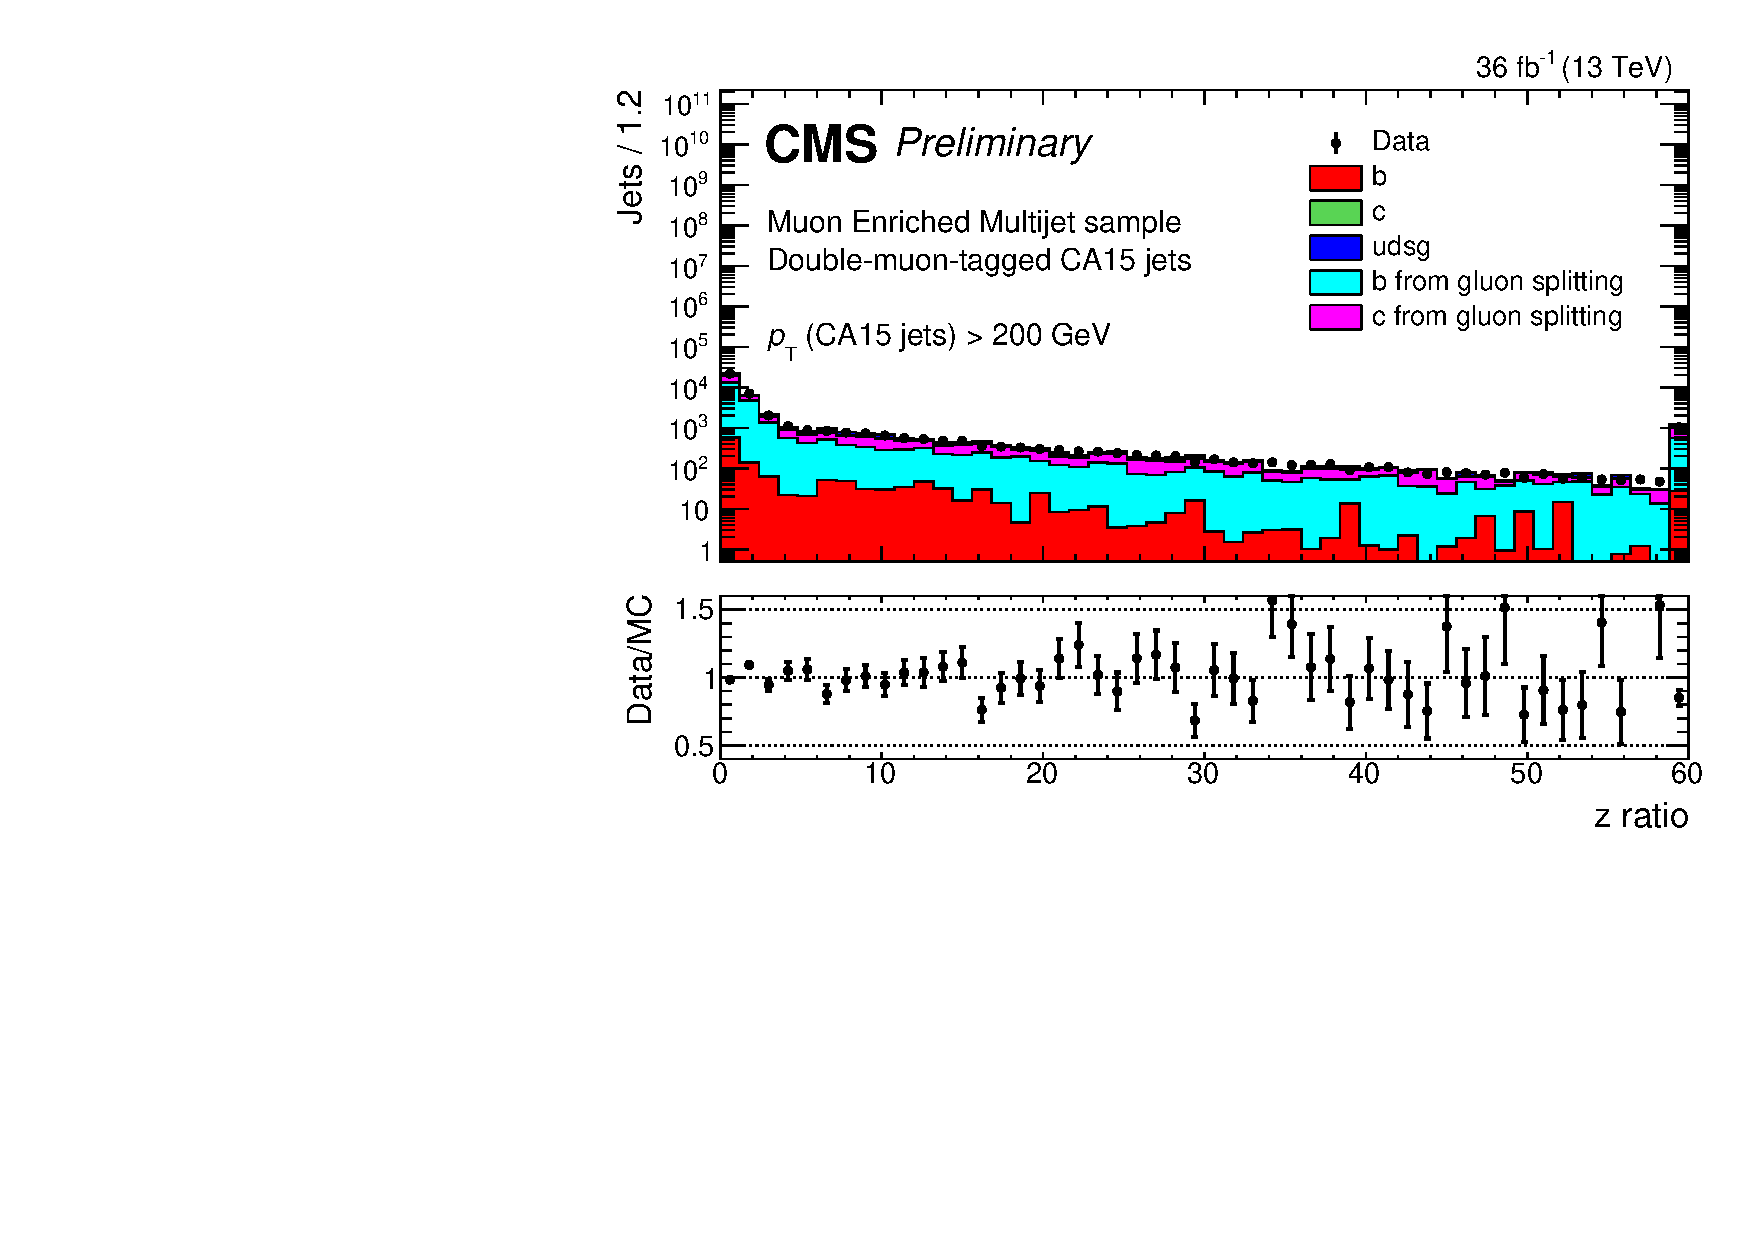
\includegraphics[width=0.475\textwidth]{figures/higgstagging/doubleb/FatJet_z_ratio_Log}}
% \subfloat{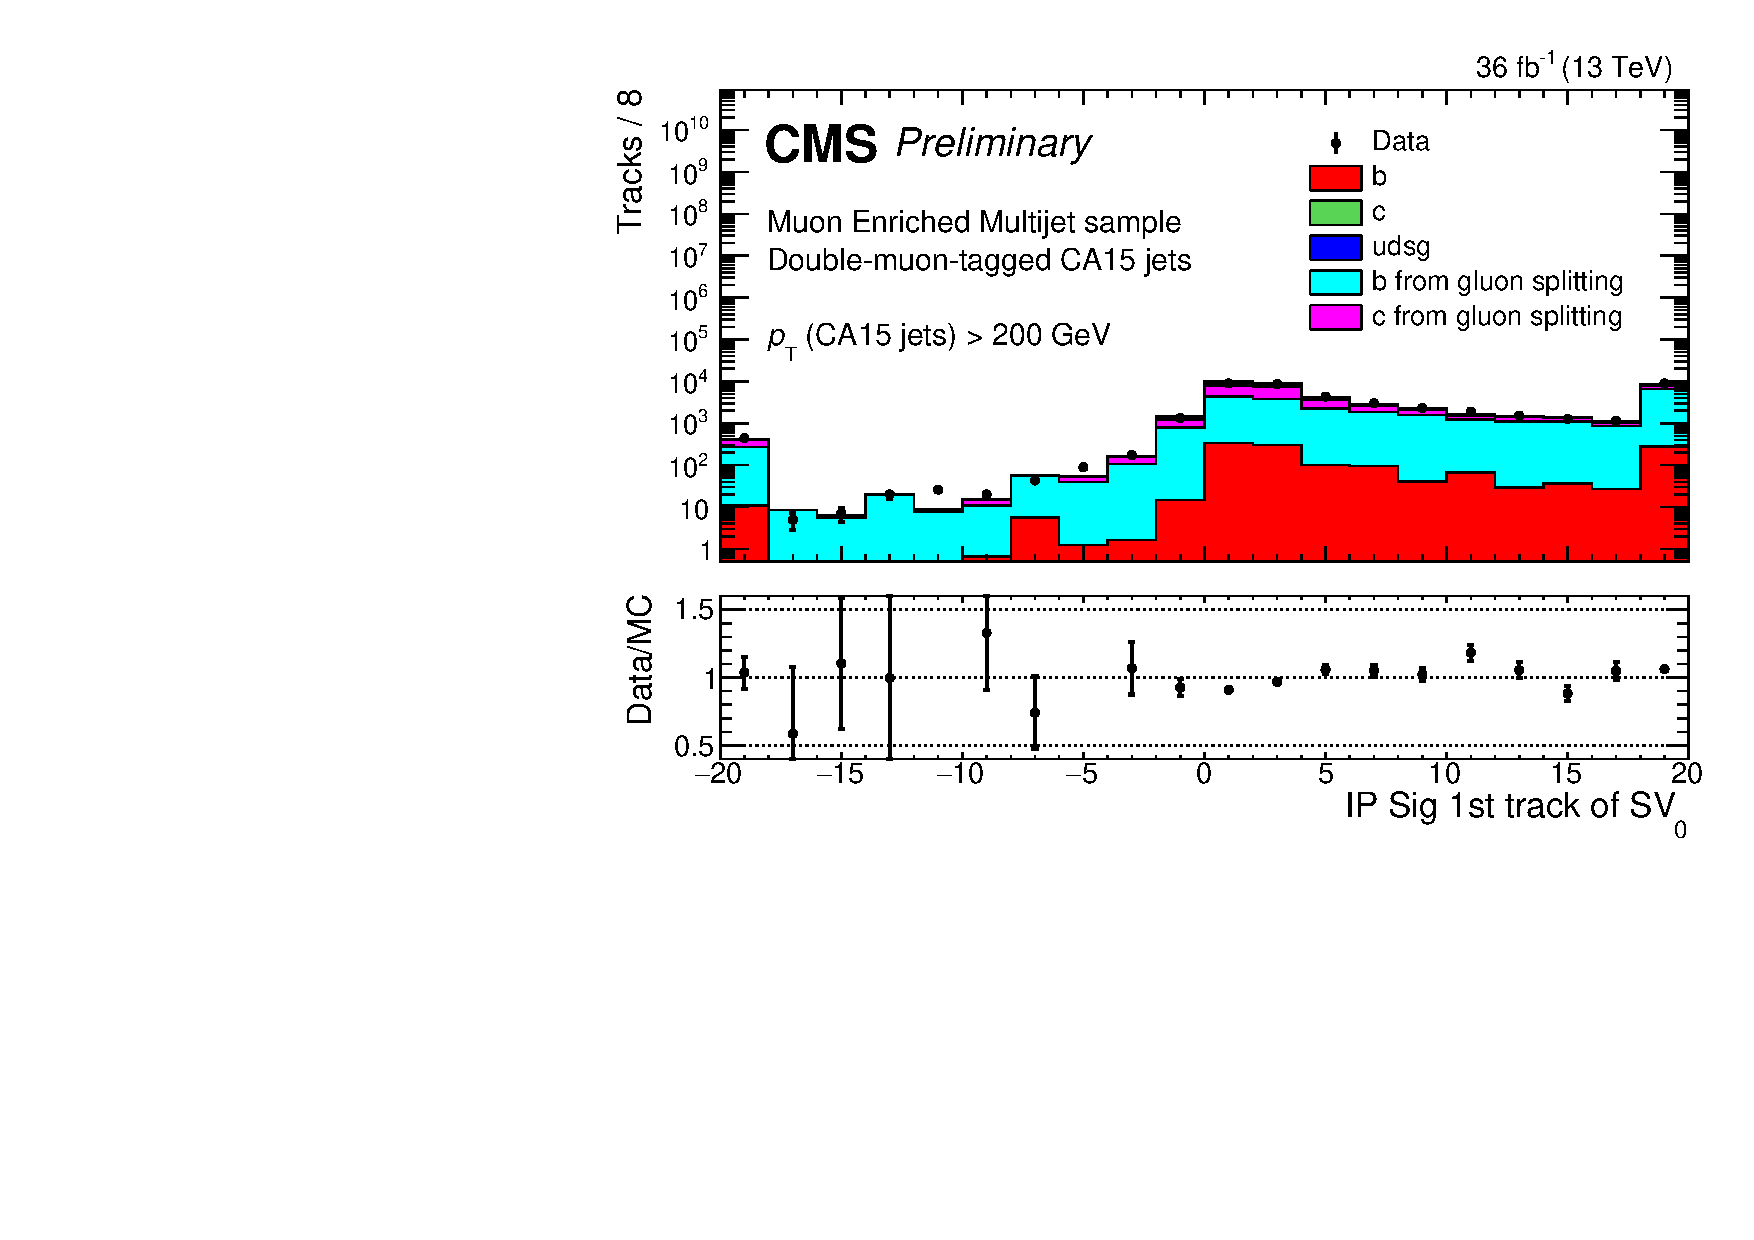
\includegraphics[width=0.475\textwidth]{figures/higgstagging/doubleb/FatJet_tau1_trackSip3dSig_0_Log}}\\
% \subfloat{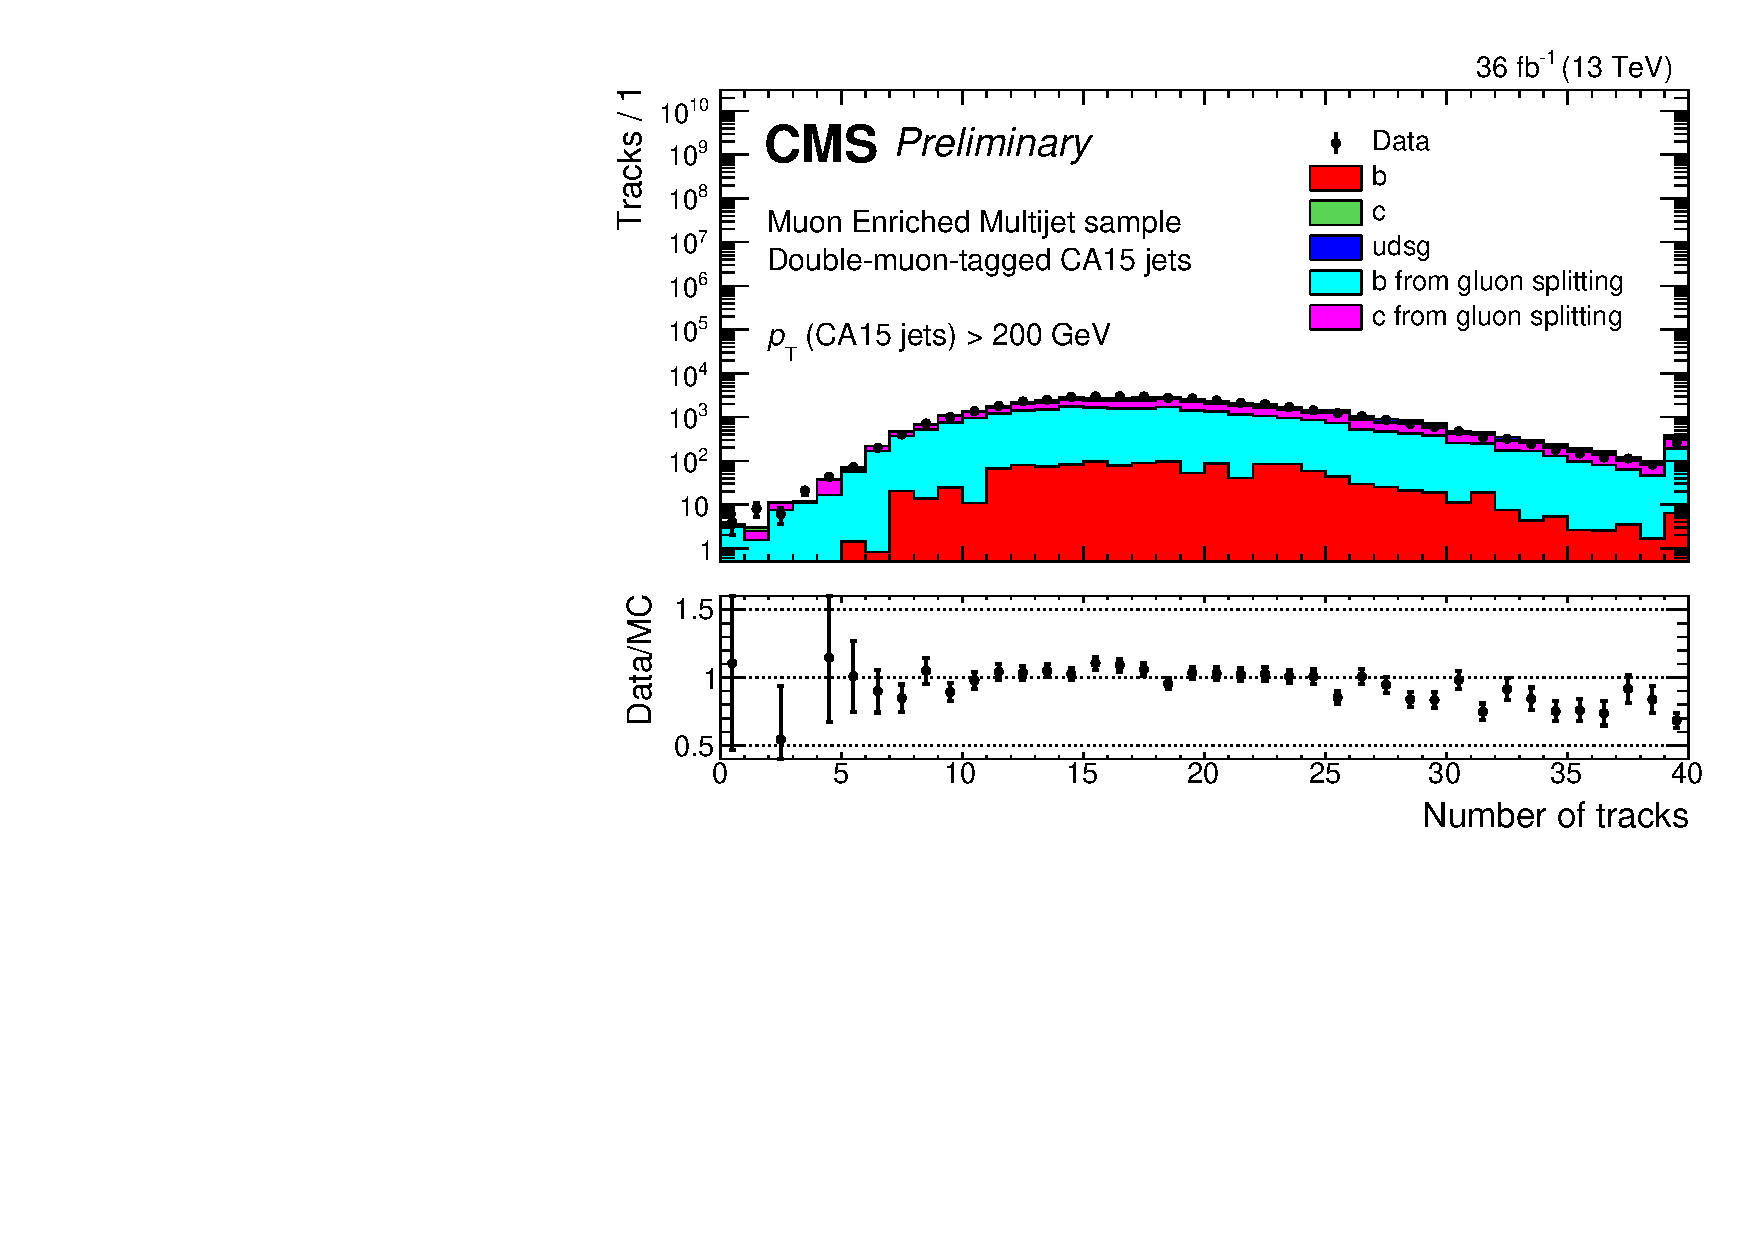
\includegraphics[width=0.475\textwidth]{figures/higgstagging/doubleb/FatJet_jetNTracks_Log}}
% \subfloat{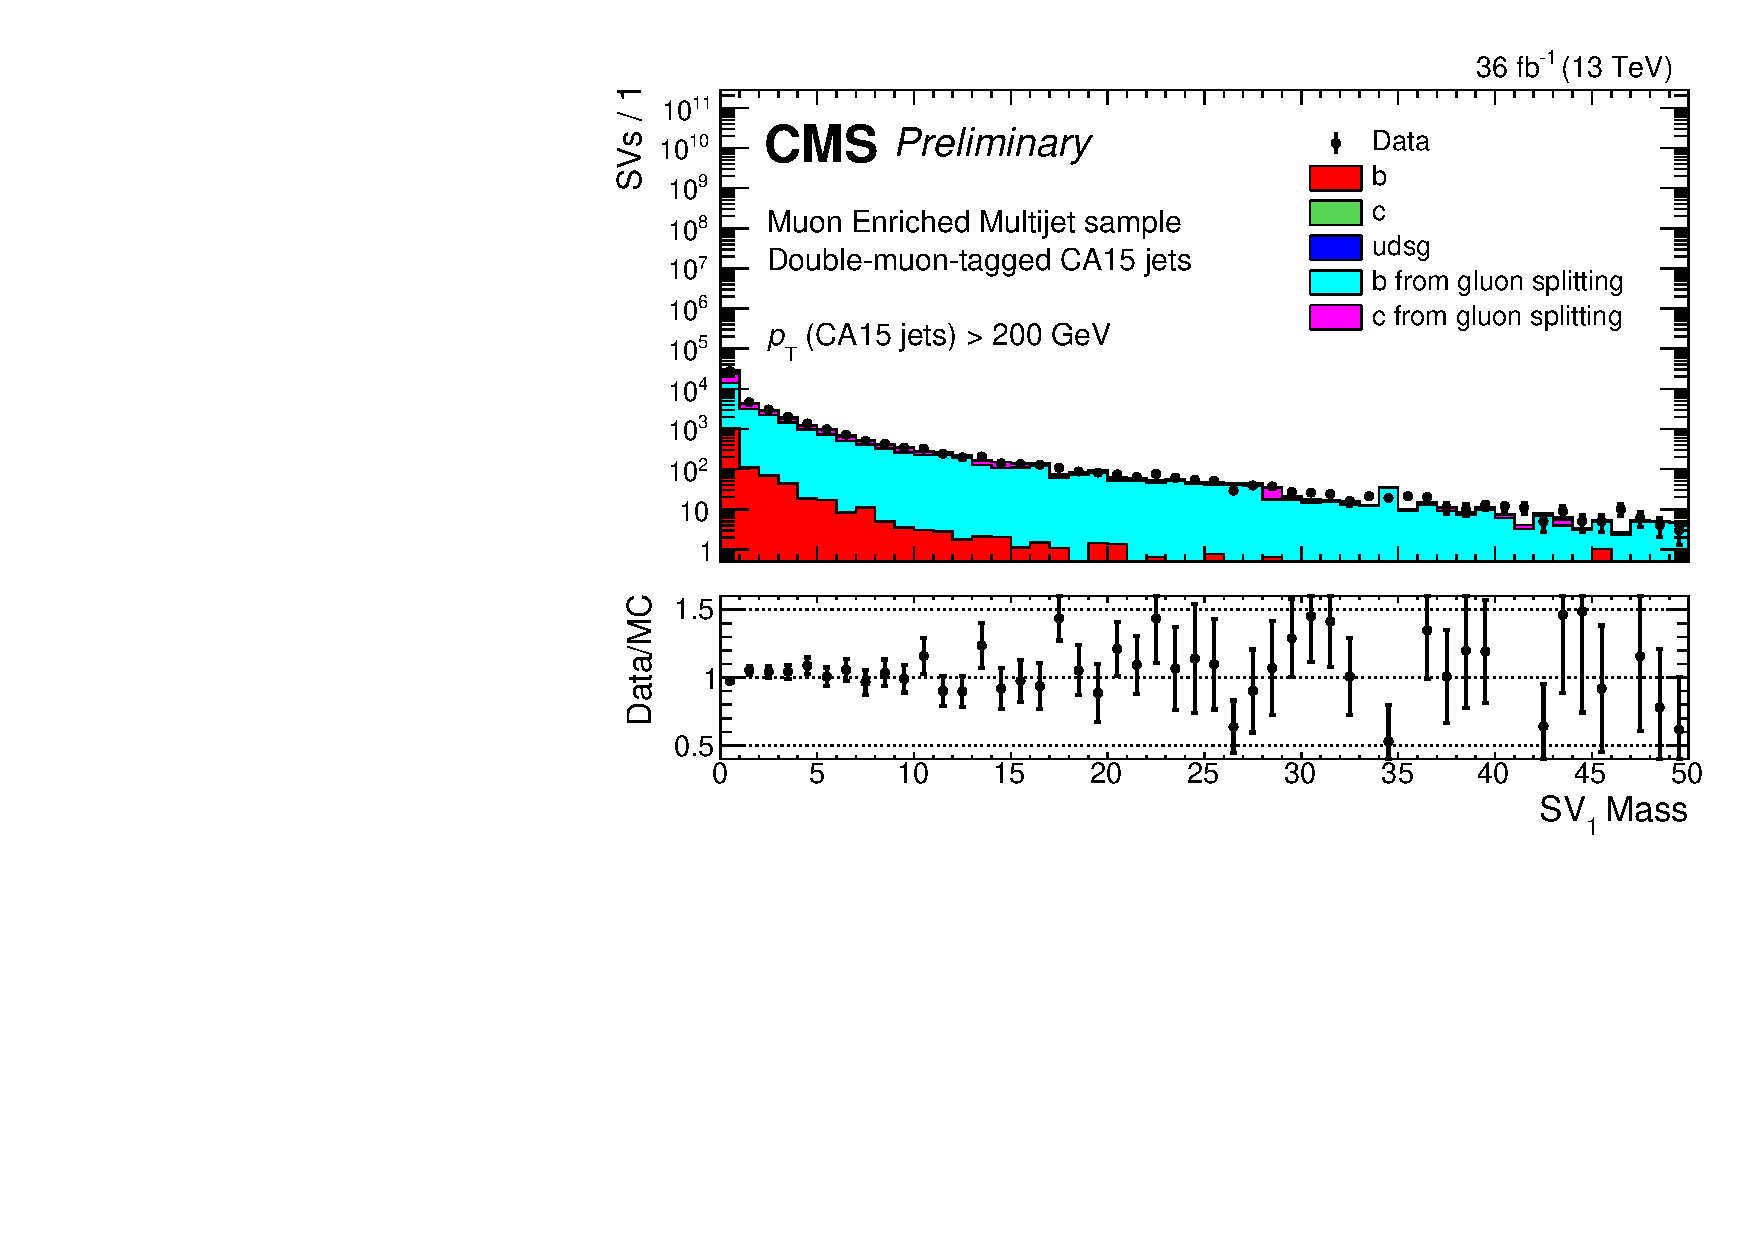
\includegraphics[width=0.475\textwidth]{figures/higgstagging/doubleb/FatJet_tau2_vertexMass_Log}}\\
% \subfloat{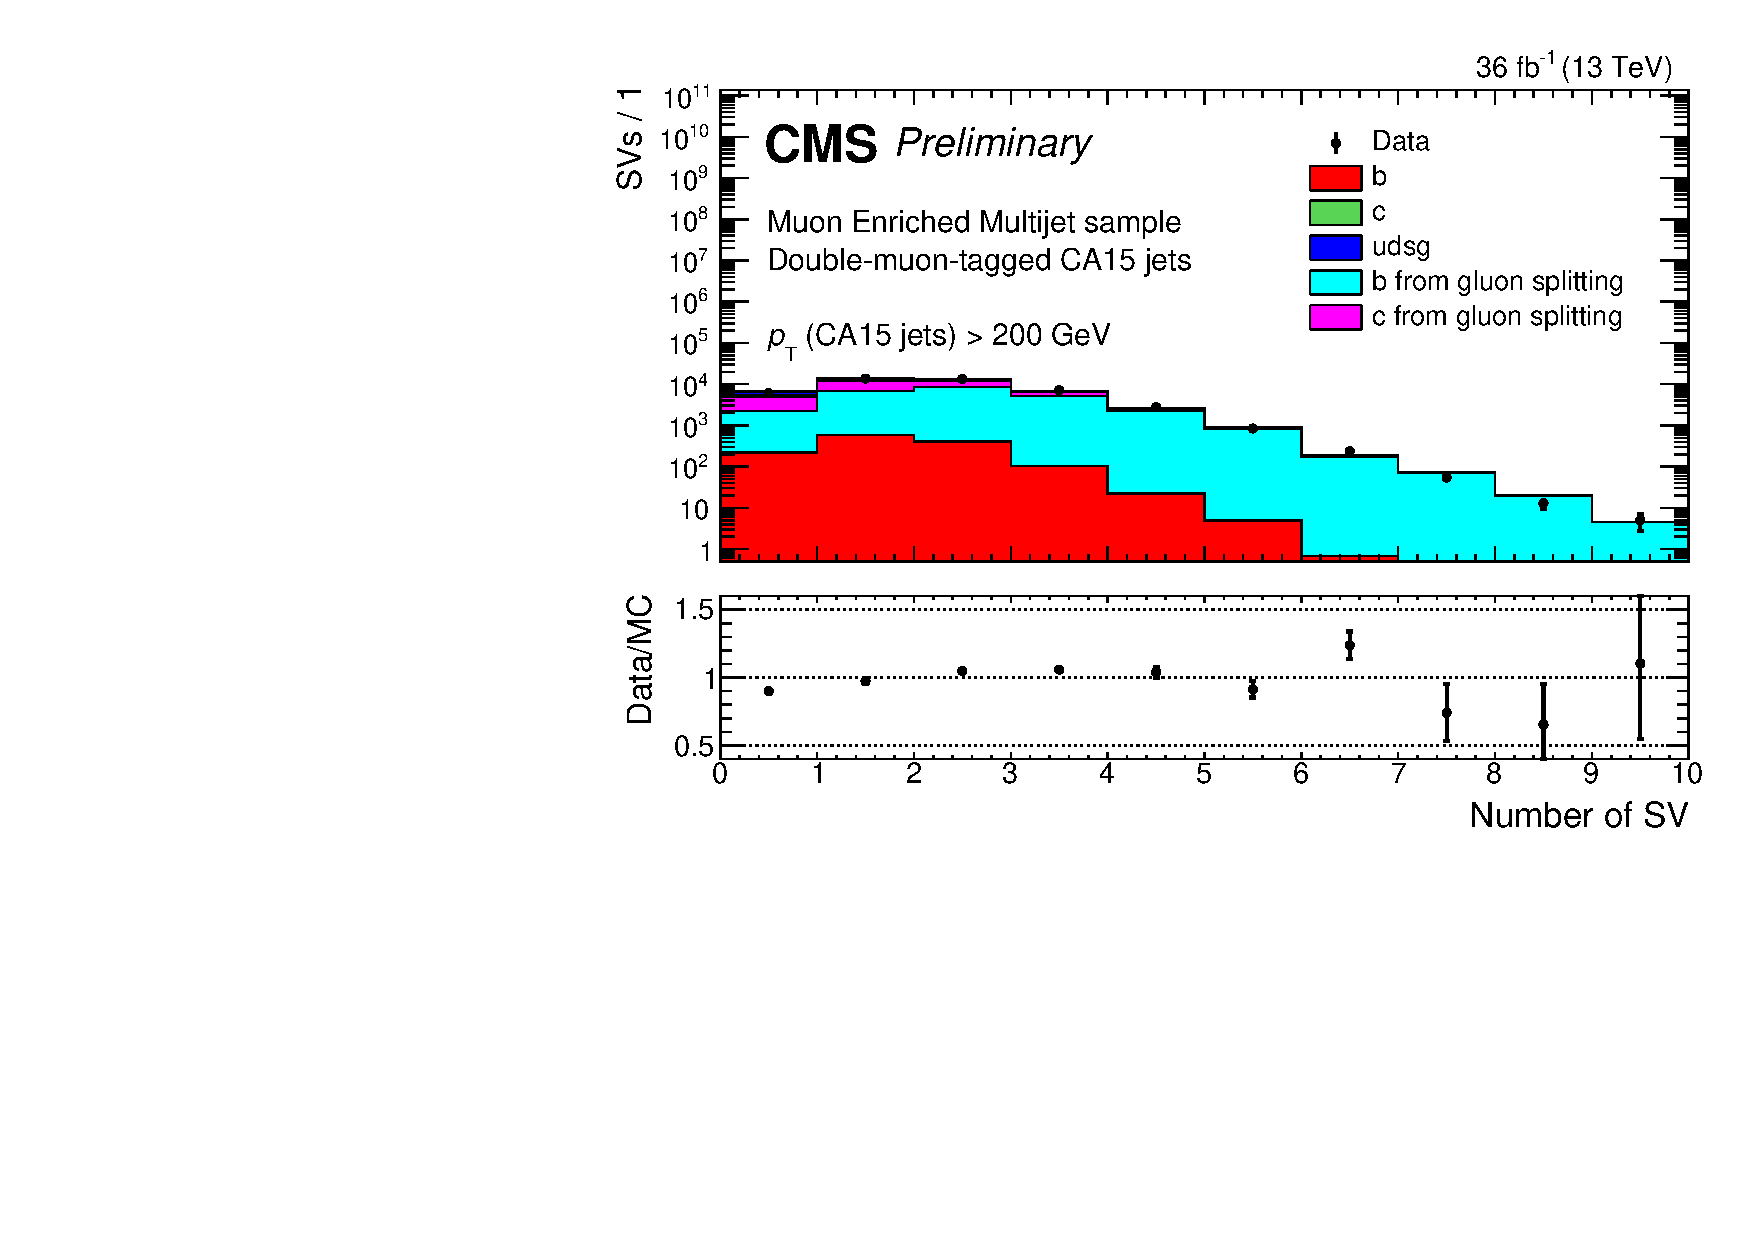
\includegraphics[width=0.475\textwidth]{figures/higgstagging/doubleb/FatJet_nSV_Log}}
% \subfloat{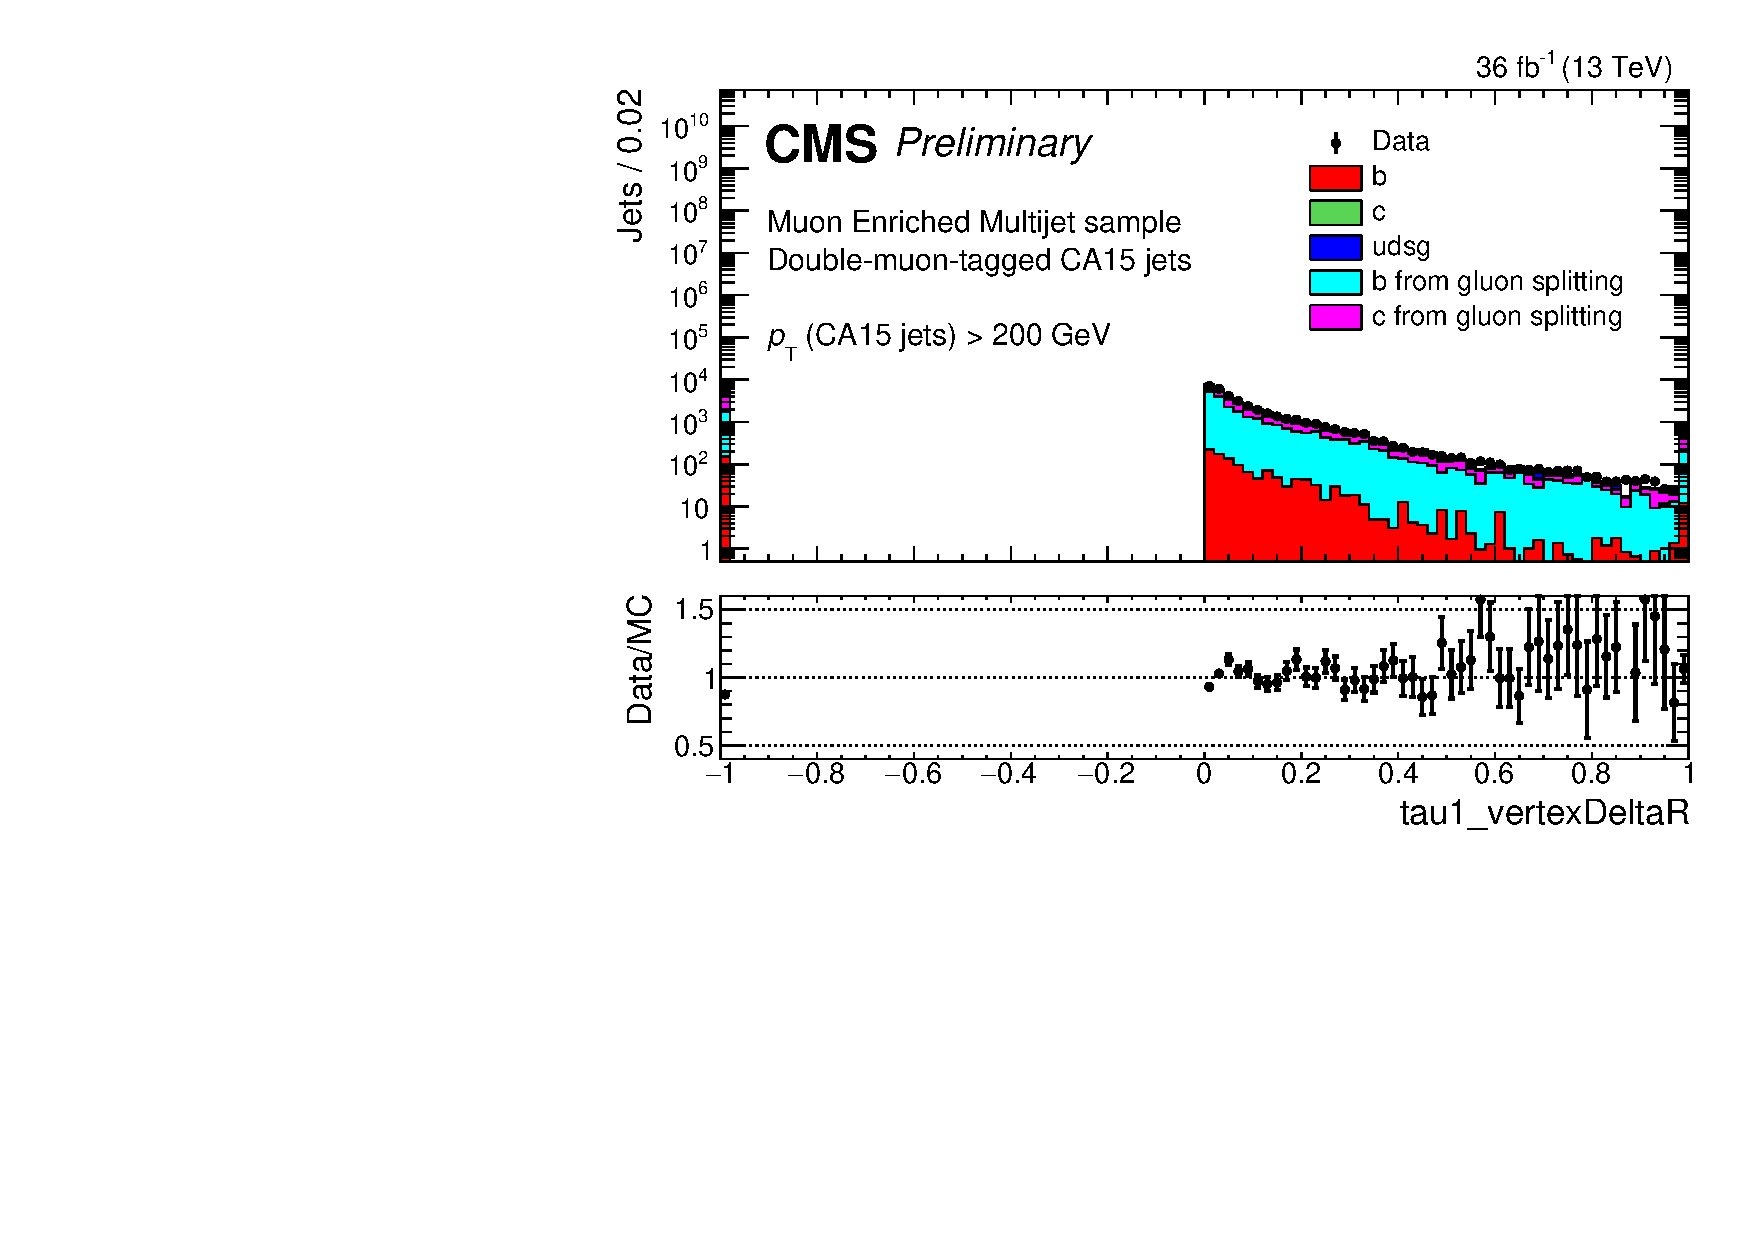
\includegraphics[width=0.475\textwidth]{figures/higgstagging/doubleb/FatJet_tau1_vertexDeltaR_Log}}\\
% \subfloat{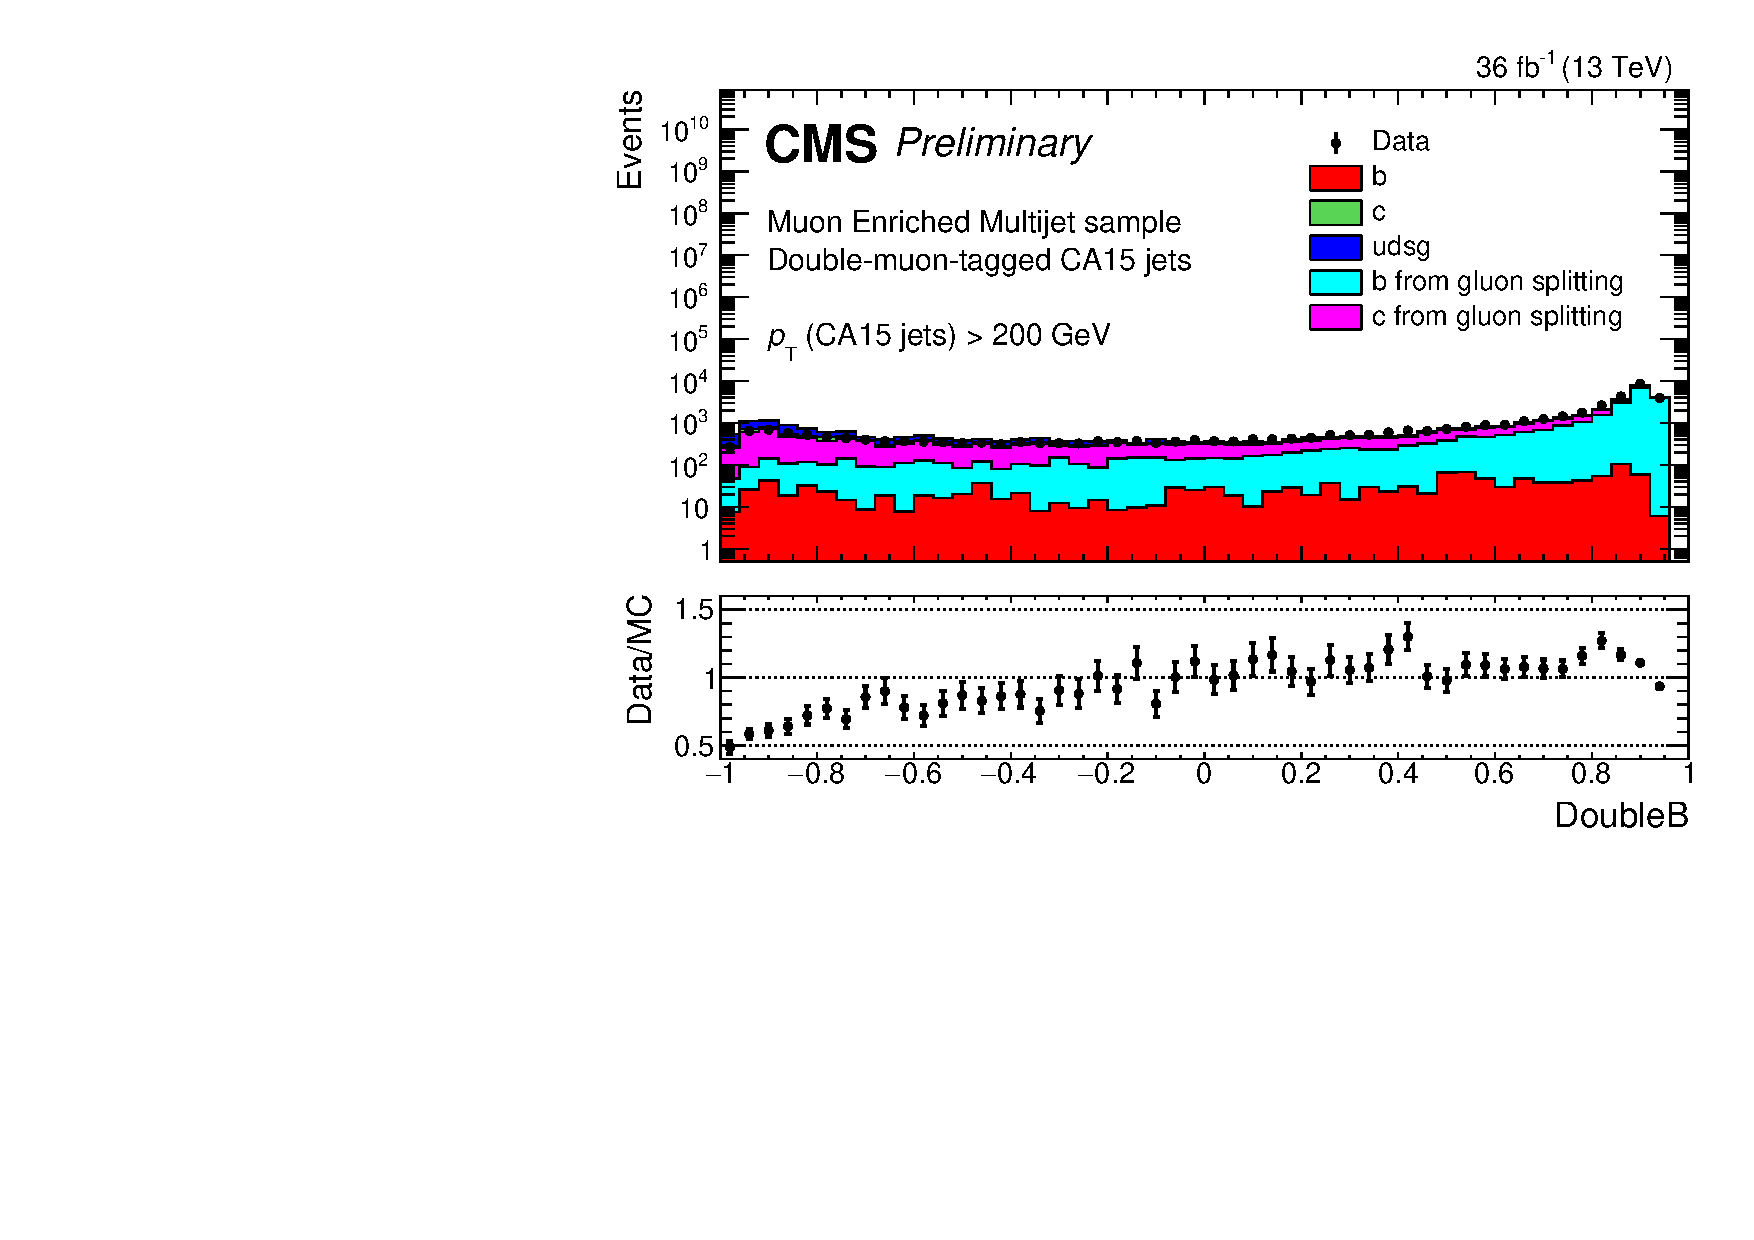
\includegraphics[width=0.475\textwidth]{figures/higgstagging/doubleb/FatJet_DoubleB_Log}}
% \subfloat{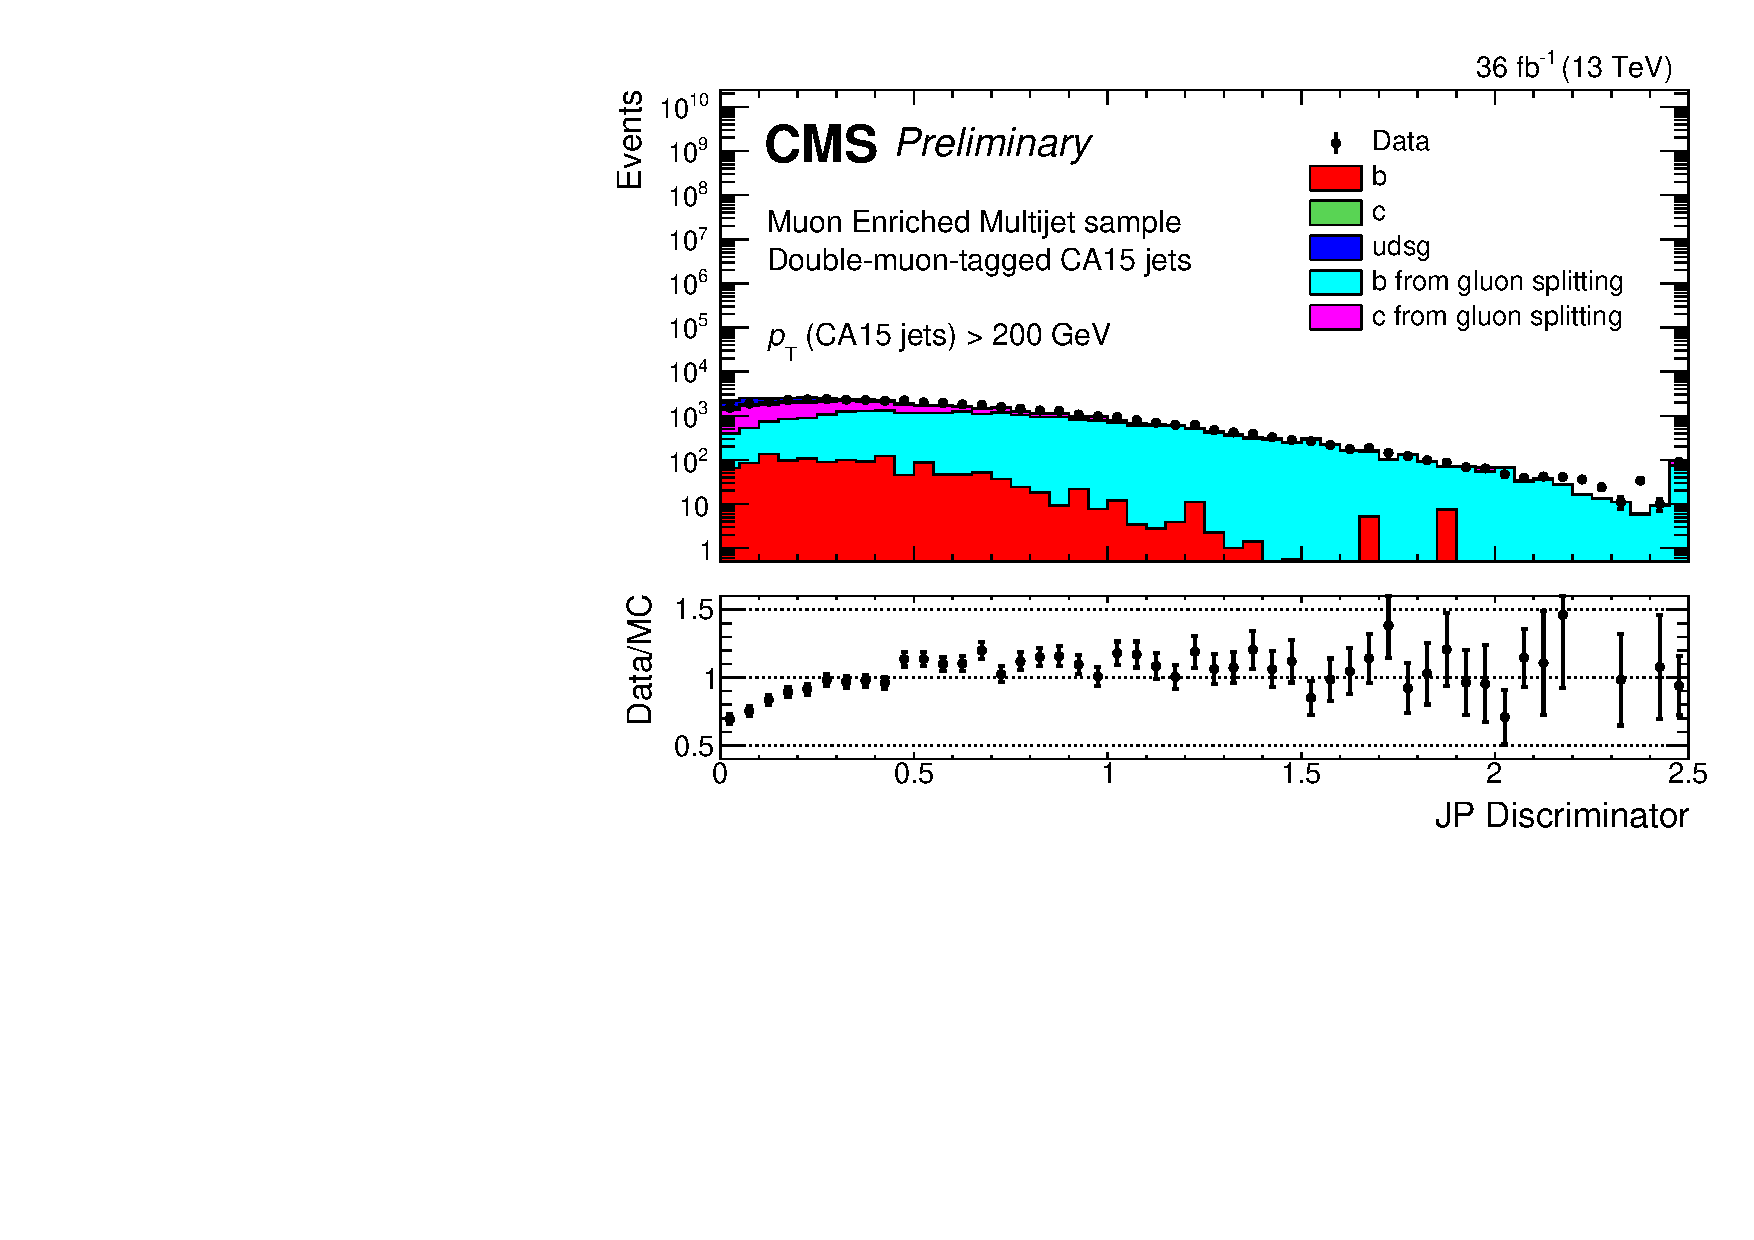
\includegraphics[width=0.475\textwidth]{figures/higgstagging/doubleb/FatJet_JP_Log}}\\
%\caption{Validation plots of some of the input variables in the double-muon tagged multijet samples. The bottom row shows the resulting double-b tagger distribution and the JP.}
%\label{fig:doublebdata_1}
%\end{figure}

%\begin{figure}
%\centering
% \subfloat{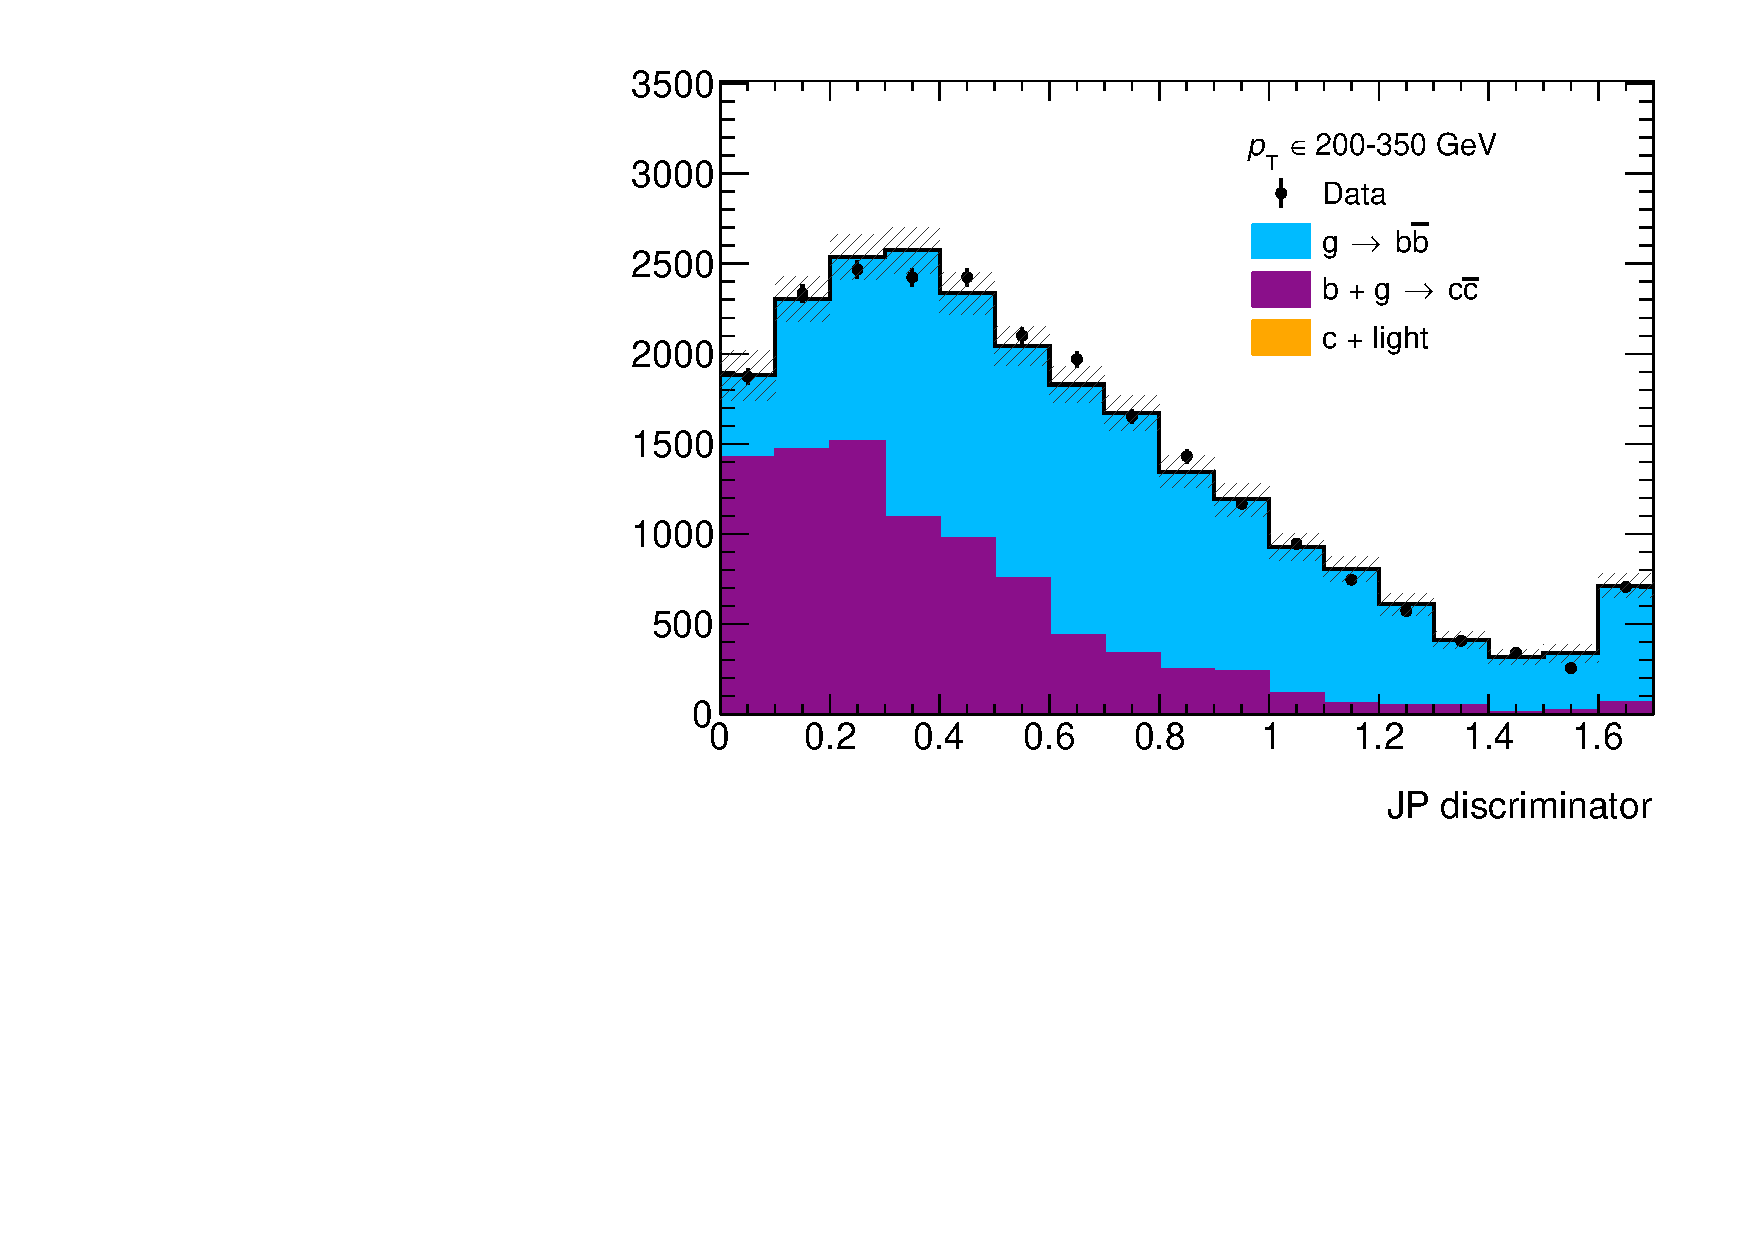
\includegraphics[width=0.45\textwidth]{figures/higgstagging/doubleb/doubleBM2ptlow/pics/result.pdf}}
% \subfloat{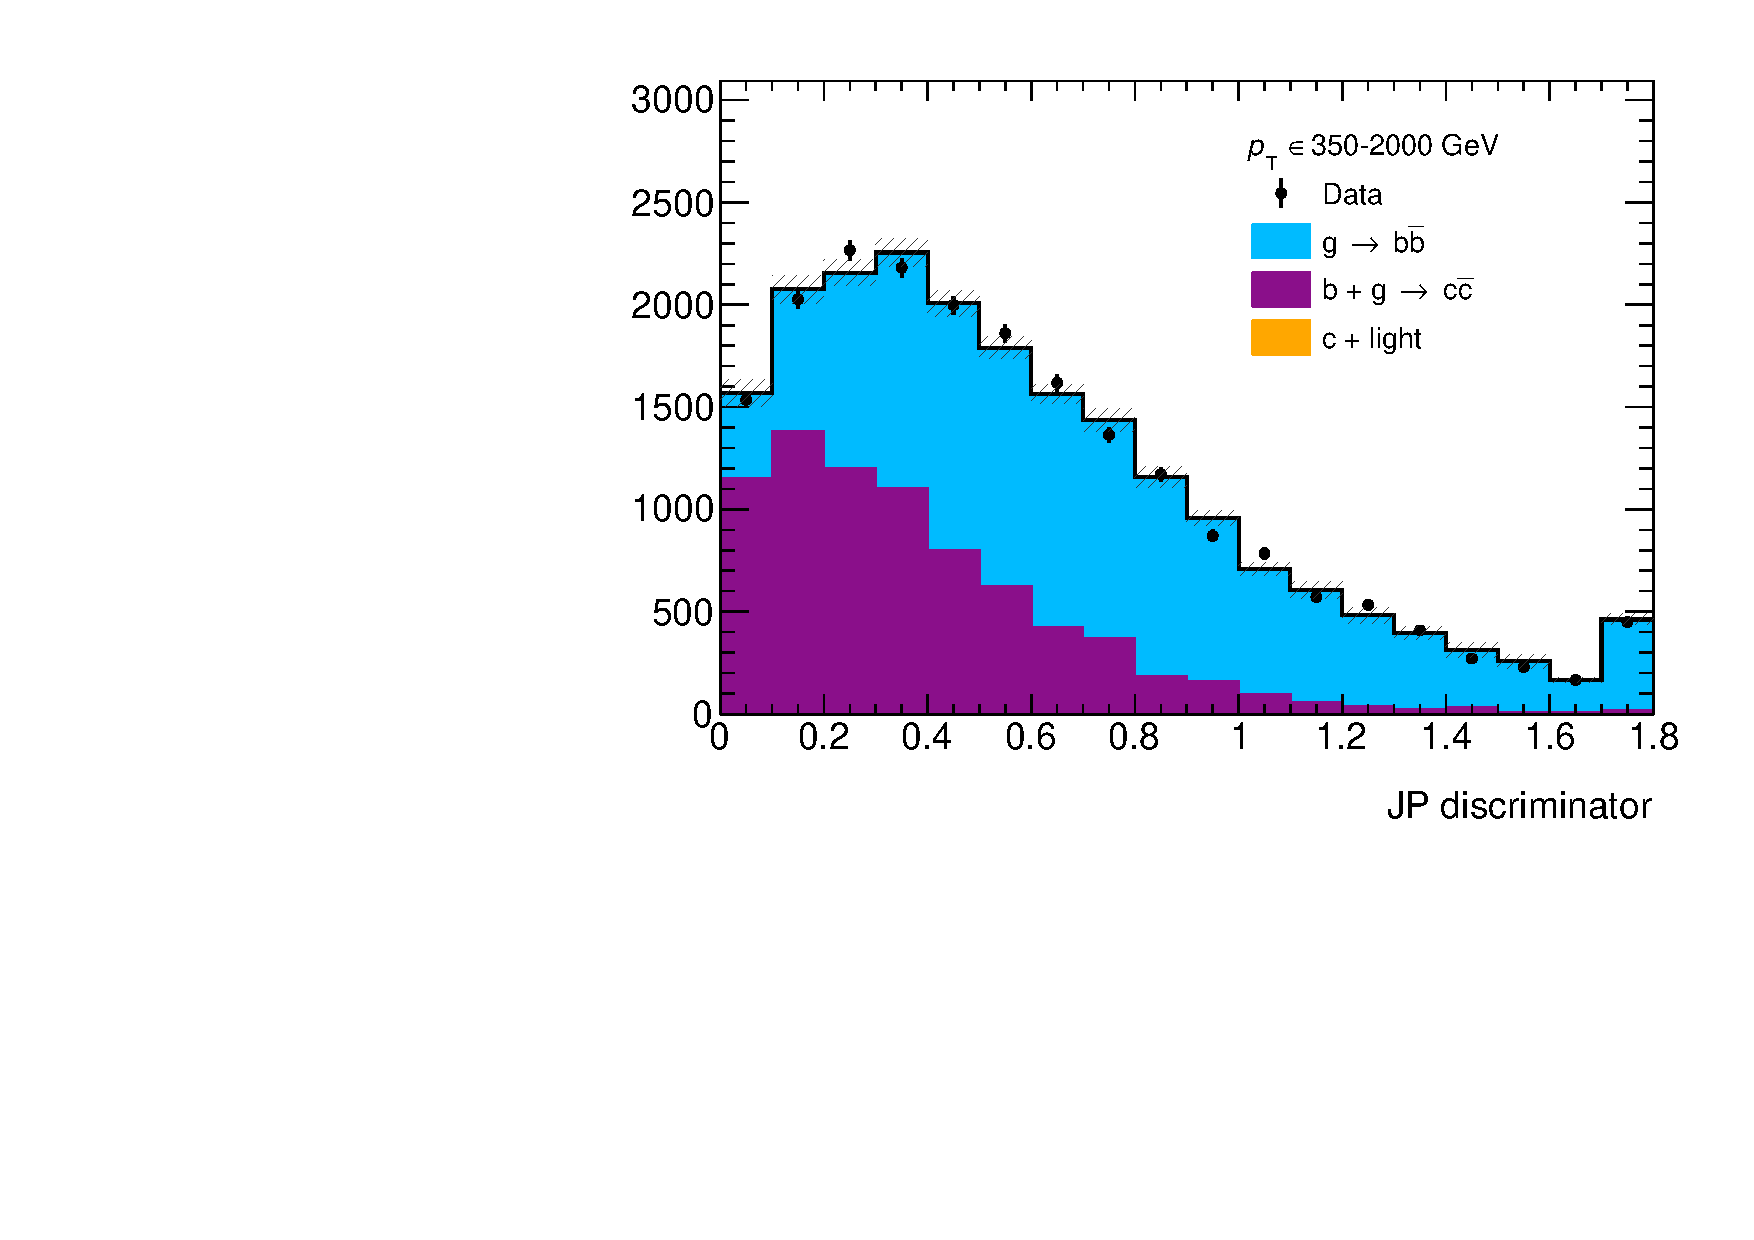
\includegraphics[width=0.45\textwidth]{figures/higgstagging/doubleb/doubleBM2pthigh/pics/result.pdf}}\\
% \subfloat{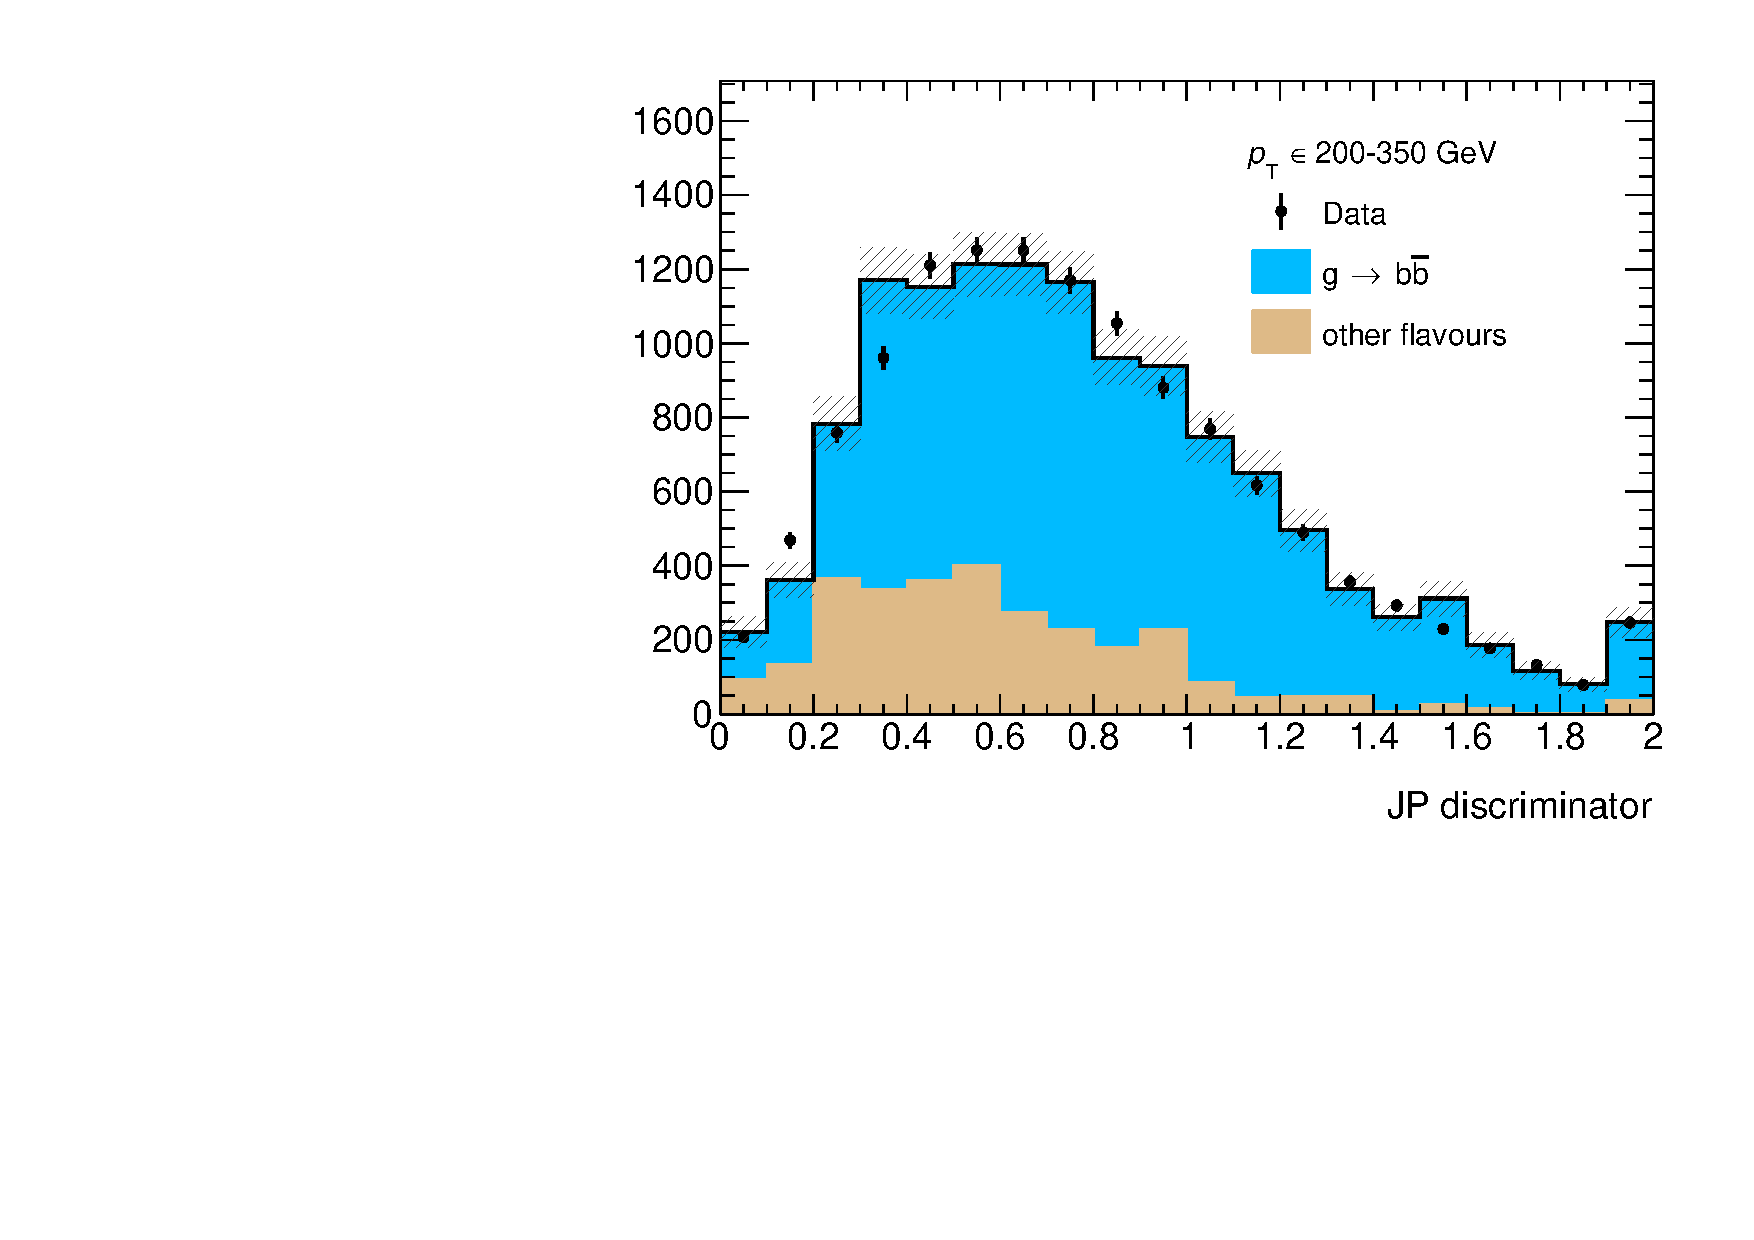
\includegraphics[width=0.45\textwidth]{figures/higgstagging/doubleb/doubleBM2ptlow/pics/result_tag.pdf}}
% \subfloat{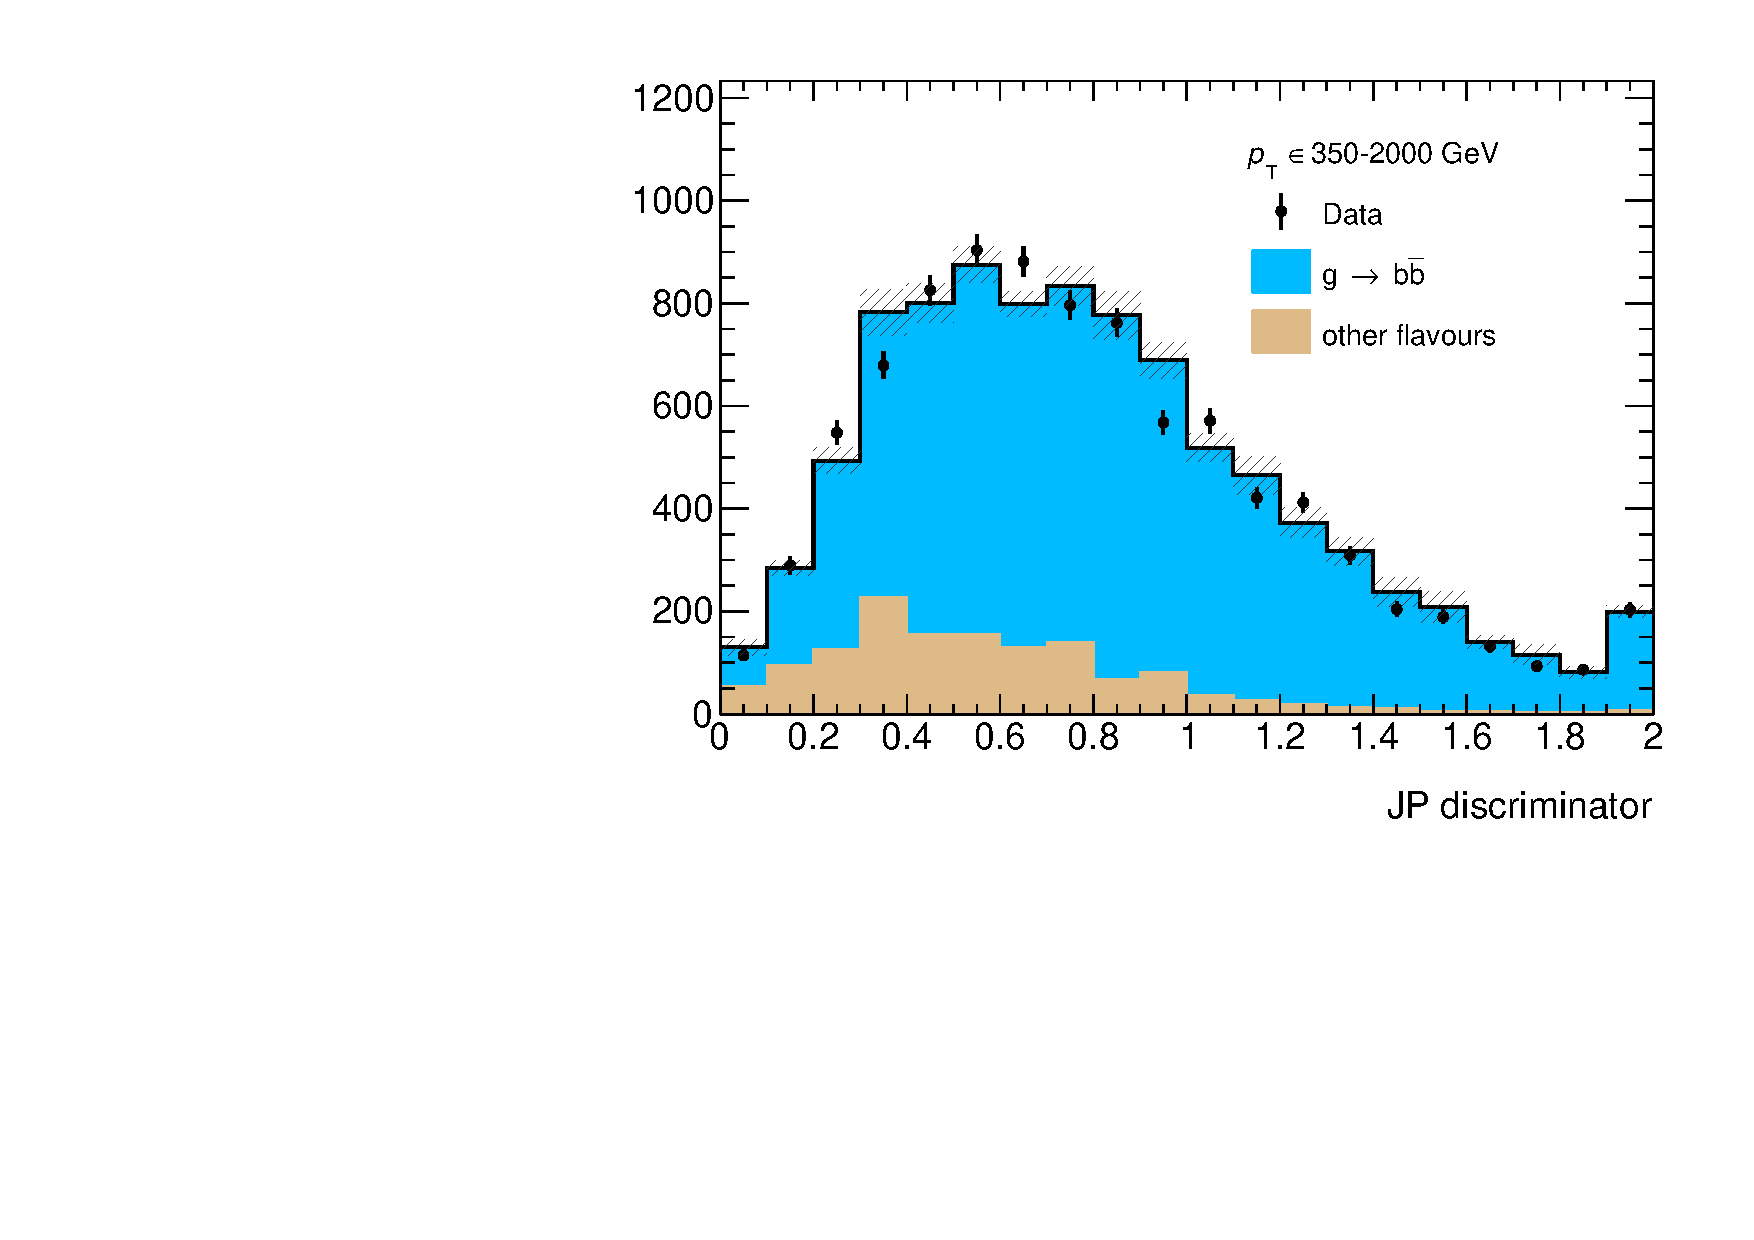
\includegraphics[width=0.45\textwidth]{figures/higgstagging/doubleb/doubleBM2pthigh/pics/result_tag.pdf}}\\
%\caption{Top row: pre-double-b-tag postfit JP distributions. Bottom row: postfit JP distributions of the events passing the double-b cut. Very good postfit agreement is observed for both the low ($<350\GeV$) and high ($>350\GeV$) \pt region.}
%\label{fig:doublebdata_2}
%\end{figure}



%\begin{table}[htbH]\footnotesize
%  \begin{center}
%  \topcaption{Fit results for the efficiency scale factor measurement corresponding to a double-b cut $>0.75$.}
%  \label{tab:Doubleb_FitParameters1}
%  \begin{tabular}{  l | c  | c | c  | c | c | c | c }
%  \hline
%  \hline
%     $p_\text{T}$ (GeV) & $\chi^2/\text{NDoF}$ & $\epsilon$ (MC) & $\epsilon$ (data) & \textbf{SF} &stat & sys up & sys down\\ \midrule
%     \hline
%200-350 & 1.04& $0.71\pm0.01$ & $0.65\pm0.04$ &  $\textbf{0.91}\pm\textbf{0.03}$ &  0.029 & 0.011 & 0.019\\ \hline

%$>350$ & 1.91 & $0.61\pm0.01$ & $0.61\pm0.03$ & $\textbf{1.00}\pm\textbf{0.04}$ & 0.024 & 0.013 & 0.032\\ \hline
%     \hline
%     \hline
%  \end{tabular}
%  \end{center}
%\end{table}


%\subsubsection{Mistagging efficiency measurement for top quark jets}
%\label{mistag_efficiency}

%One dominant source of background is semi-leptonic \ttbar production where the lepton is lost either because it is out of acceptance or does not pass the criteria imposed in the selection. In the mass window between 100\GeV and 150\GeV, the absolute fake rate of top quark induced fat jets for the chosen double-b working point is about 14\%. With the top quark being resonantly produced in the vicinity of the our signal region mass window (as opposed to the combinatorial background arising from QCD radiation inducing fat jets such as, for example, in Z+jets), we perform a dedicated mistag measurement for the top quark induced fat jets, following the strategy of~\cite{CMS-PAS-BTV-15-002}. We define a \ttbar enriched region orthogonal to our nominal top control region introduced in Section~\ref{sec:cr} by inverting the requirement on the number of allowed additional AK4 jets and by widening the window on the fat jet soft drop mass to 50-250\GeV. This ensures a flavor composition in the fat jets that is similar to the one found in our signal region, which is mostly comprised of fat jets that contain the b quark and one light quark of the top quark (and subsequent W boson) decay.


%\begin{figure}[h]
%\centering
%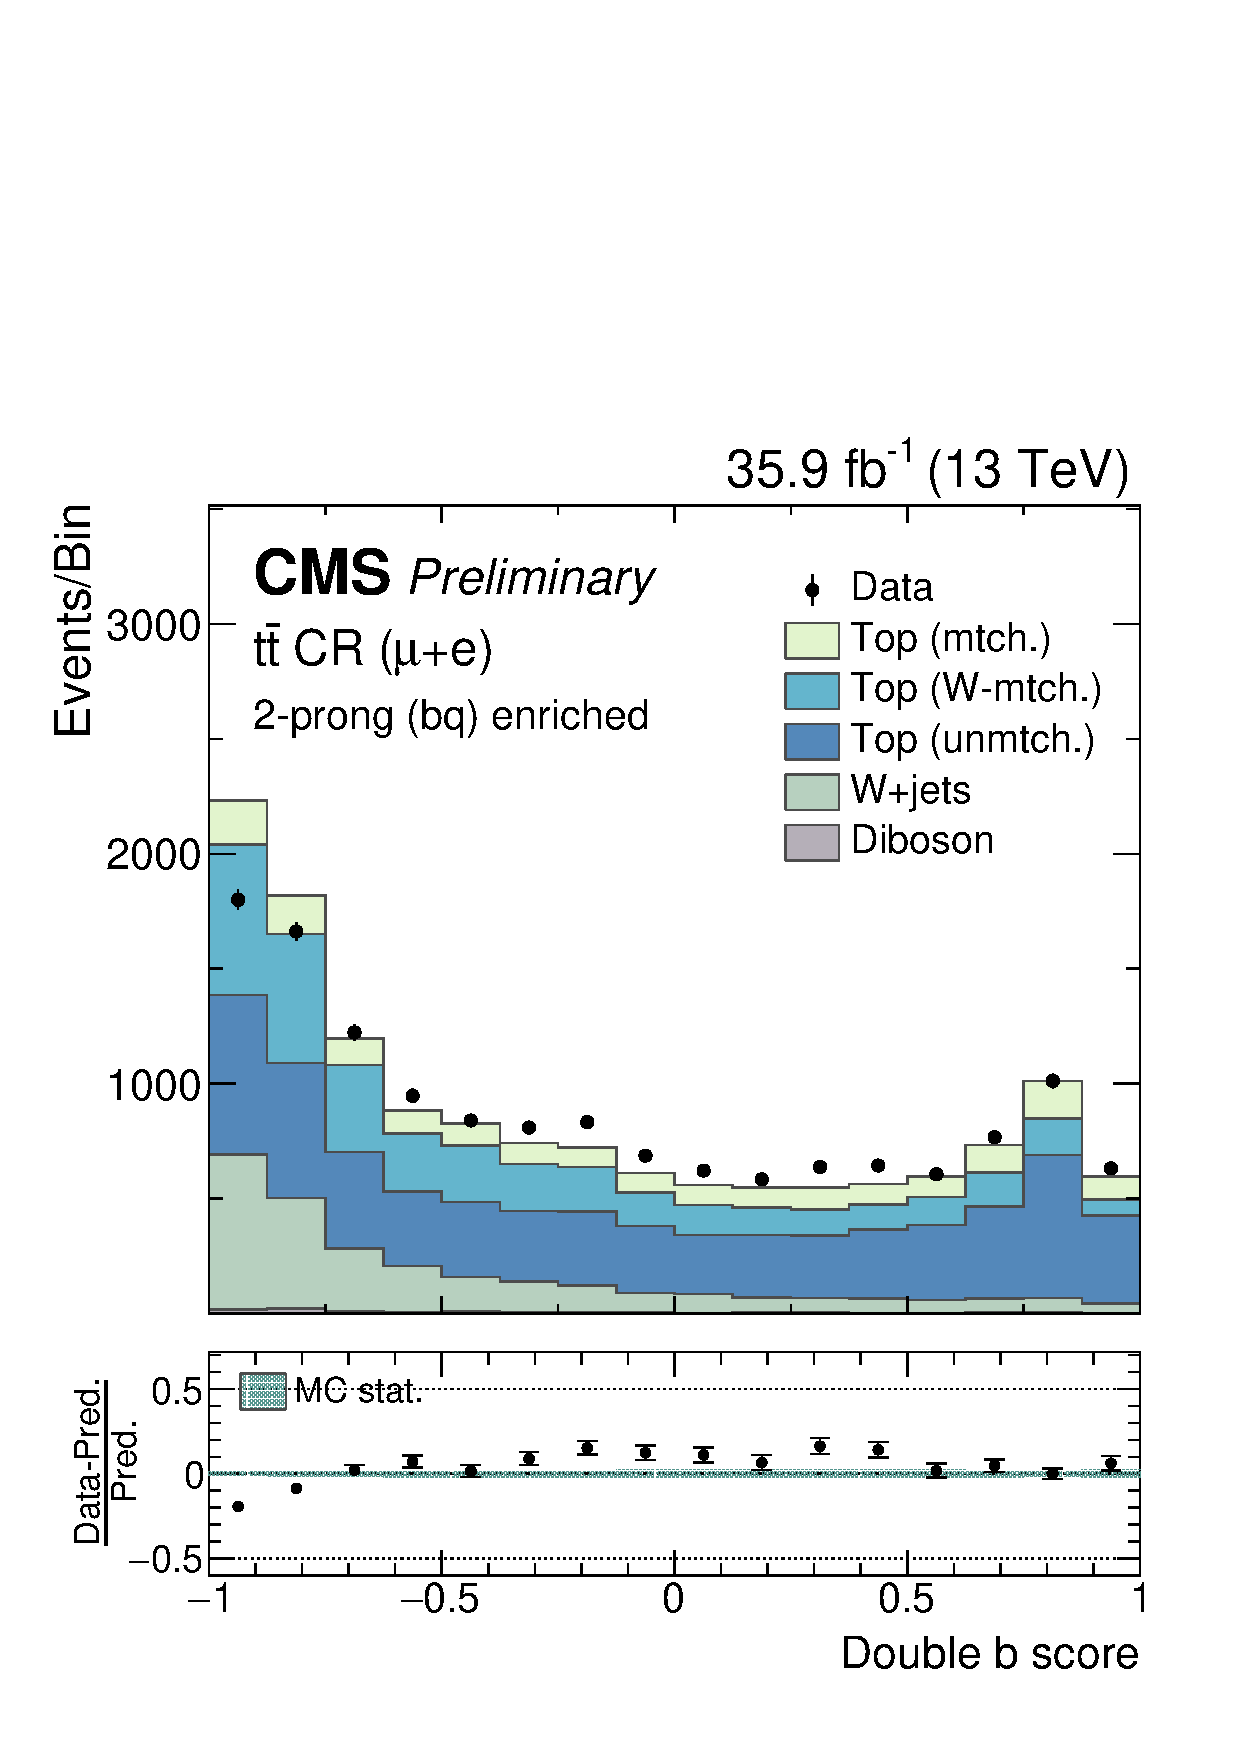
\includegraphics[width=0.45\textwidth]{figures/dataMC/cr_ttbar_mu_fj1DoubleCSV_2prong.pdf}
%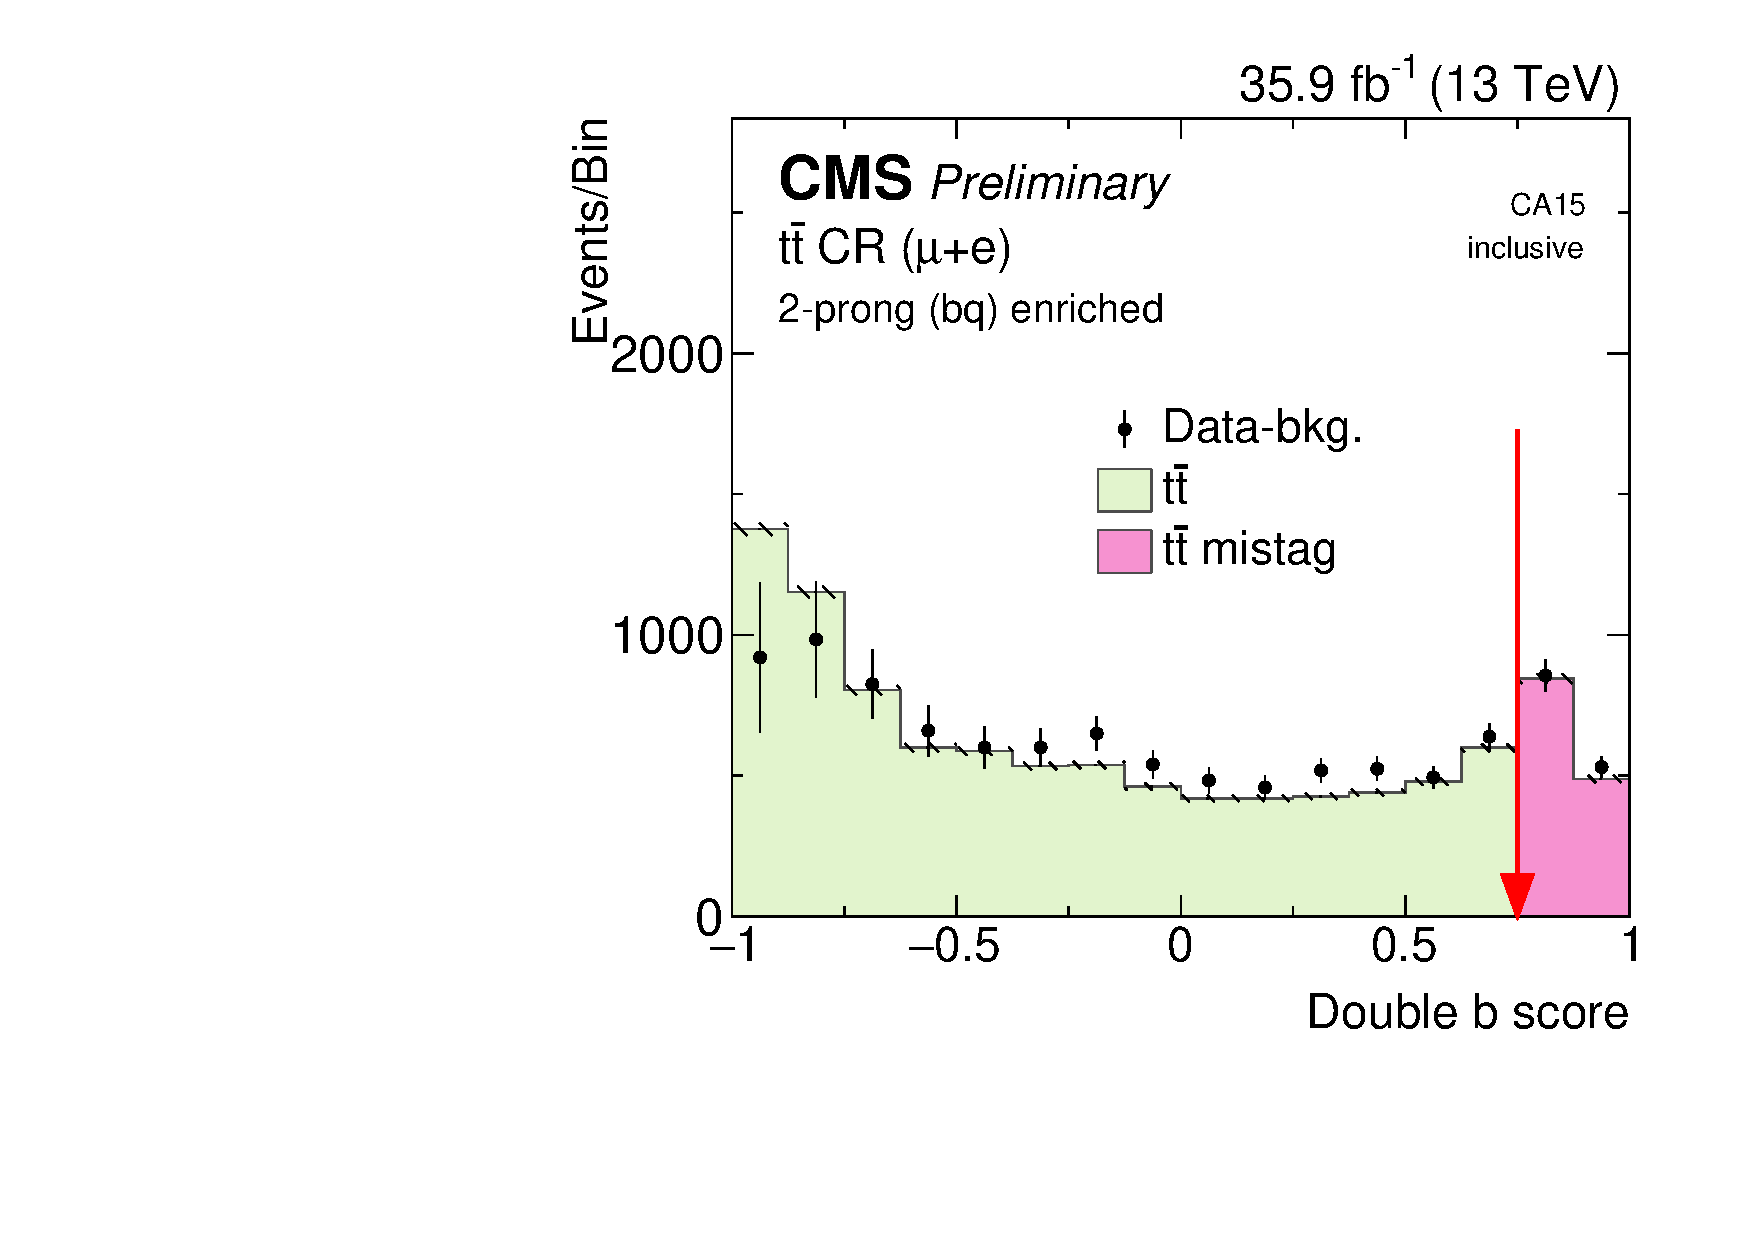
\includegraphics[width=0.45\textwidth]{figures/higgstagging/cr_ttbar_mu_fj1DoubleCSV.pdf}\\
%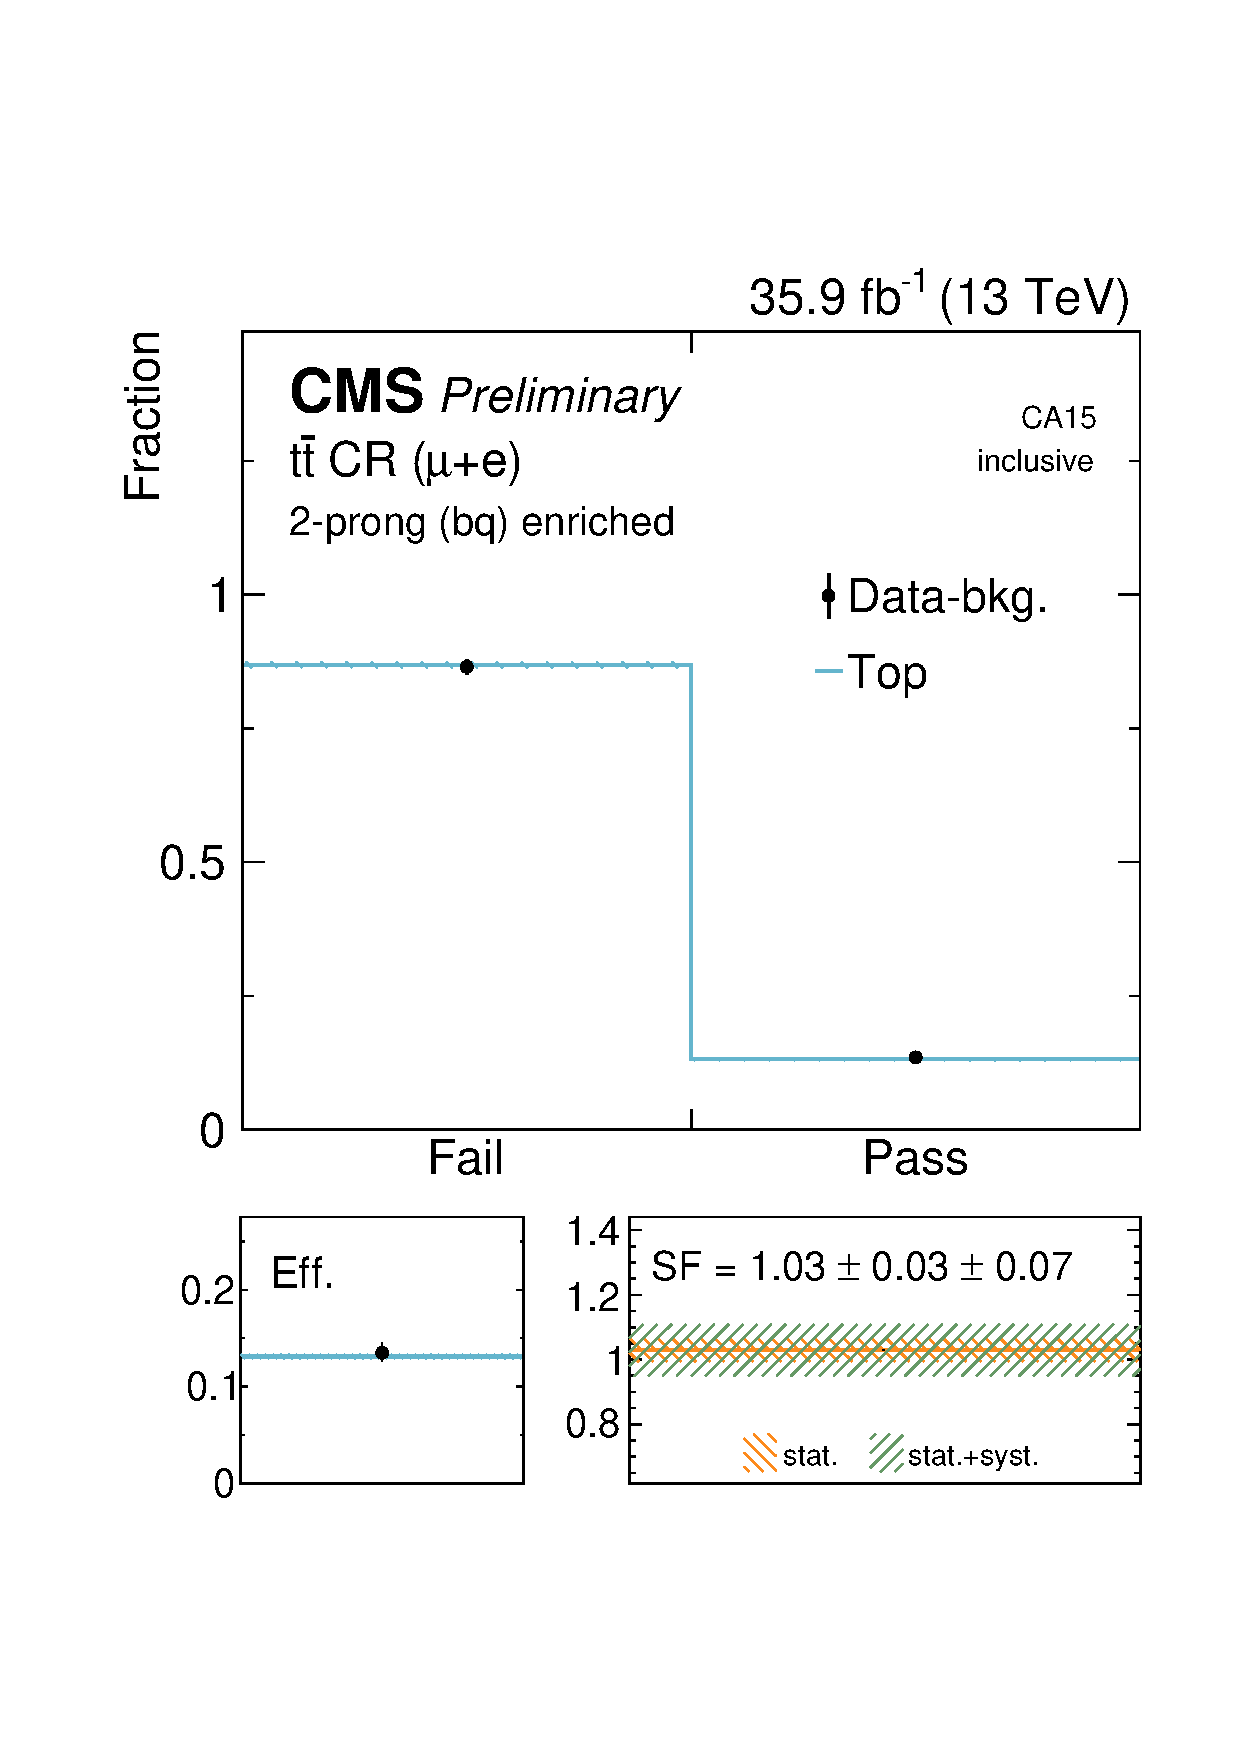
\includegraphics[width=0.4\textwidth]{figures/dataMC/cr_ttbar_mu_fj1DoubleCSV_sf.pdf}\\
%\caption{Top row: data vs. MC comparison in the combined e+$\mu$ \ttbar~CR with inverted requirement on the number of isolated AK4 jets (left). The ``Top'' templates contain contributions from both \ttbar and single top processes.  They are split up into different quark content of the fat jet. Just as for the signal region, the main contribution comes from events with ``unmatched'' top quarks where the fat jet contains a b and a light quark. Background-subtracted data (i.e. data minus W+jets, single top, diboson predictions) is compared to only the \ttbar simulation (this time not split up) in the upper right figure, from which the scale factor is computed. The red arrow indicates the double-b working point. Bottom row: the scale factor is given by the ratio of efficiencies of double-b score $>0.75$ in data and MC.}
%\label{fig:ttbarmistag}
%\end{figure}

%Then, all non-\ttbar background is subtracted from data, and the mistag SF is given by the ratio of efficiencies found in background-subtracted data and \ttbar simulation, as shown in Figure~\ref{fig:ttbarmistag}. A 30\% uncertainty on the subtracted backgrounds (mostly single top and W+jets) is applied, resulting in a scale factor of $1.03\pm0.03(\text{stat.})\pm0.07(\text{syst.})$. The \ttbar~reweighting has been applied in this measurement. Not applying this correction results in a 1\% effect on the scale factor; we therefore neglect this source of systematic uncertainty. 

%The scale factor will serve as prior for the parameter that extracts the relative normalization of \ttbar between bins passing or failing the double-b cut in-situ from the maximum-likelihood fit described in Section~\ref{sec:results}.

%A measurement binned in fat jet \pt gives consistent results and is found to have no impact on the final sensitivity of the analysis. All \ttbar mistag scale factors are listed in Table~\ref{tab:Doubleb_FitParameters2}.


%\begin{table}[htbH]
%  \begin{center}
%  \topcaption{Mistag scale factor measurement for top quark jets.}
%  \label{tab:Doubleb_FitParameters2}
%  \begin{tabular}{  l | c  | c | c  }
%  \hline
%  \hline
%     $p_\text{T}$ (GeV) & \textbf{SF} &stat & sys \\ \midrule
%     \hline
%inclusive & $\textbf{1.03}$ & 0.03 & 0.07\\ \hline
%200-350 & $\textbf{1.04}$ & 0.04 & 0.07\\ \hline
%350-500 & $\textbf{1.00}$ & 0.07 & 0.08\\ \hline
%$>500$ & $\textbf{1.02}$ & 0.17 & 0.21\\ 
%     \hline
%     \hline
%  \end{tabular}
%  \end{center}
%\end{table}


